% GENERATED from neurips_arxiv.tex by make. Edit neurips_arxiv.tex, not this file.
\documentclass{article}

% arXiv preprint: un-anonymizes via [preprint] option per NeurIPS 2026 handbook.
\usepackage[main, final]{neurips/neurips_2026}

\usepackage{amsmath, amssymb, amsthm}
\usepackage{graphicx}
\graphicspath{{../figures/}}
\usepackage{booktabs}
\usepackage{hyperref}
\usepackage{multirow}
\usepackage{array}
\usepackage{subcaption}
\usepackage{float}
\usepackage{xcolor}
\usepackage{bm}
\usepackage{tikz}
\usetikzlibrary{arrows.meta, positioning, fit, backgrounds, calc}
\usepackage{titlesec}

% Whitespace tightening (defaults LaTeX leaves alone; .sty already tightens captions/lists/math)
\setlength{\textfloatsep}{8pt plus 2pt minus 2pt}
\setlength{\intextsep}{8pt plus 2pt minus 2pt}
\setlength{\floatsep}{8pt plus 2pt minus 2pt}
\titlespacing*{\section}{0pt}{8pt plus 2pt minus 2pt}{4pt plus 1pt minus 1pt}
\titlespacing*{\subsection}{0pt}{6pt plus 1pt minus 1pt}{3pt plus 1pt minus 1pt}
\titlespacing*{\paragraph}{0pt}{4pt plus 1pt minus 1pt}{1em}

\newtheorem{definition}{Definition}
\newtheorem{proposition}{Proposition}
\newtheorem{assumption}{Assumption}

\DeclareMathOperator{\Var}{Var}
\DeclareMathOperator{\Cov}{Cov}
\DeclareMathOperator{\E}{E}

% NeurIPS-style answer macros (used in the paper checklist)
\providecommand{\answerYes}[1][]{\textcolor{blue}{[Yes]}#1}
\providecommand{\answerNo}[1][]{\textcolor{red}{[No]}#1}
\providecommand{\answerNA}[1][]{\textcolor{gray}{[NA]}#1}
\providecommand{\answerTODO}[1][]{\textcolor{orange}{[TODO]}#1}

% Public code repository (real GitHub URL for the preprint)
\newcommand{\codeurl}{\url{https://github.com/SolomonMg/totalevalerror}}
\newcommand{\codeurltext}{github.com/SolomonMg/totalevalerror}

\title{Hidden Measurement Error in LLM Pipelines Distorts Annotation, Evaluation, and Benchmarking}

\author{%
  Solomon Messing\thanks{Corresponding author.} \\
  Center for Social Media, AI, and Politics, New York University \\
  MLCommons \\
}

\begin{document}

\maketitle

\begin{abstract}
LLM evaluations drive model deployment, safety standards, research conclusions, and future projections, for example, about AI's impact on the labor market. Yet the way we often estimate noise from autoraters (LLM-as-judge) ignores variability from factors like judge model choice and prompt phrasing, which means we're underestimating error in a way that \emph{worsens} with more data. This unmeasured variance can affect results enough to reverse conclusions \citep{baumann2025llmhacking, huang2026dropping}. And judge-pipelines that fail to average this variation are more vulnerable to ``benchmark hacking'' \citep{singh2025leaderboard}. This paper introduces a framework we call ``total evaluation error (TEE),'' which decomposes LLM pipeline uncertainty and uses design-study projections to reduce total error. In our safety and ideology applications, naive standard errors are 53 - 70\% smaller than the corrected SE under our TEE framework. Using Chatbot Arena data, we show naive 95\% CI coverage drops as $n$ grows, while TEE-corrected coverage holds at 95\%, and TEE-guided pipelines restrict the potential range of benchmark gaming by roughly 43\%. We show further that a small pilot allows for the estimation of proper CIs, with the added benefit of projecting which design changes most improve precision. Using those projections to allocate API calls cut MMLU estimation error roughly in half against the answer key at the same budget, and increased per-match agreement with human voters on Chatbot Arena by 7.9 percentage points.
\end{abstract}

\section{Introduction}
\label{sec:intro}

LLM measurement pipelines introduce variance at multiple stages that traditional reporting norms ignore. Researchers who use LLMs for annotation, evaluation, or content moderation routinely do so with no assessment of prompt sensitivity, temperature dependence, or item-level heterogeneity \citep{pecher2026underspecification, barrie2025replication}. Benchmark scores likewise depend on prompt wording and scoring model choice, and this dependence is seldom measured (SI Appendix, Table~\ref{tab:current_practice}).\footnote{AlpacaEval and Chatbot Arena report item-sampling CIs; AILuminate uses a multi-judge evaluator ensemble; no benchmark decomposes prompt, temperature, or interaction variance. Full survey of 10 benchmarks and 3 annotation studies in SI Appendix, Table~\ref{tab:current_practice}.} In all cases, unmeasured variation can create analogues to $p$-hacking \citep{simmons2011falsepositive, gelman2013garden} and overfitting \citep{recht2019imagenet} such that the results reflect measurement noise, not general phenomena.

At best, current practice reports confidence intervals (CIs) reflecting variation from repeated sampling at identical settings, ignoring prompt sensitivity, item heterogeneity, and their interactions. Figure \ref{fig:underestimation} presents simulation results showing that we should expect under-coverage to \emph{worsen} with more items, because omitted variance from prompt and judge choices does not shrink with~$N$.\footnote{Variance parameters estimated via REML according to the framework introduced below; 1,000 simulation replicates per data point (see Section~\ref{si:simulations} for simulation details).}

\begin{figure}[htbp]
\centering
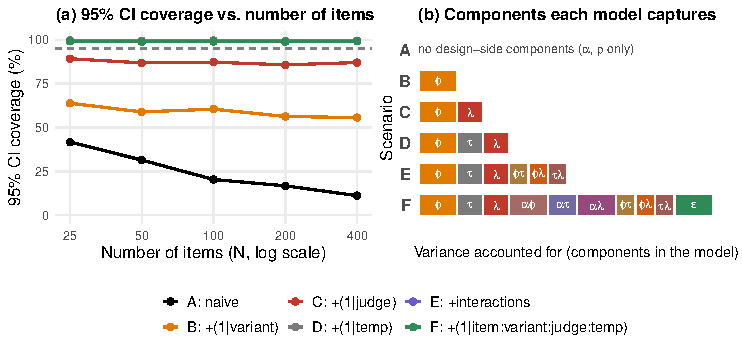
\includegraphics[width=0.9\linewidth]{fig_underestimation_slide_v2.pdf}
\caption{Naive confidence intervals fail because pipeline variance from prompt, judge, and temperature choice does not shrink with items ($N$). (a)~95\% CI coverage versus $N$ in 6 scenarios (A-F). (b)~Variance components accounted for in each scenario. Scenario A corresponds to the naive estimate $\Phi^{-1}(0.975) \times s/\sqrt{N}$; scenarios B-F represent adding more variance parameters estimated according to the framework introduced below. Scenarios D-F overlap.%Scenarios: A, $\mathrm{SE}=s/\sqrt{N}$; B adds $V=3$ prompts and fits $(1\,|\,\text{item})+(1\,|\,\text{variant})$, capturing $\phi$. C adds $M=3$ judges and $(1\,|\,\text{judge})$, capturing $\lambda$. D adds $H=3$ temperatures and $(1\,|\,\text{temp})$, capturing $\tau$. E adds $(1\,|\,\text{variant:judge}) + (1\,|\,\text{variant:temp})$ for the pairwise interactions.DGP parameters rescaled for illustrative purposes.
}
\label{fig:underestimation}
\end{figure}

The problem is especially urgent in benchmarking, where unstable scores make rank-order differences between closely spaced models (or systems under test, SUT) uninterpretable for evaluators and give model developers exploitable degrees of freedom. On stable measurement, \citet{romanou2026brittlebench} show that semantics-preserving input perturbations explain near half of performance variance, minor reorderings of answer choices shift MMLU leaderboard rankings by up to 8~positions \citep{alzahrani2024benchmarks}, and on Chatbot Arena dropping just 0.003\% of human preferences is enough to flip the top-ranked model \citep{huang2026dropping}. With respect to exploitation, \citet{singh2025leaderboard} document best-of-$K$ leaderboard gaming in production, the mechanism Section~\ref{sec:gaming} quantifies.

Ignoring this variability can harm the scientific literature as well. One re-evaluation study found 31\% of hypotheses tested with state-of-the-art LLM annotations yielded incorrect conclusions under LLM configuration variation (model, prompt), and found malicious actors could reverse the sign of 68\% of statistically significant effects through adversarial configuration selection \citep{baumann2025llmhacking}. Other work has found that formatting choices alone produced a 76-point accuracy spread \citep{sclar2024sensitivity}, while infrastructure nondeterminism produced accuracy standard deviations of up to nine percentage points even at temperature zero \citep{yuan2025numerical}.\footnote{Note that setting $T = 0$ does not eliminate underlying model uncertainty. Greedy decoding picks the highest-probability token at each step to yield a single deterministic output, even when the token distribution has high entropy, hiding the variation that sampling at $T > 0$ would show. In chain-of-thought models, greedy decoding across a long reasoning trace can also lock in early token choices that do not reflect the broader distribution of answers \citep{renze2024temperature}.}

\section{Related Work}
\label{sec:related}

Several concurrent works address components of this problem, including variance decomposition \citep{haase2026withinmodel, wang2024measuring}, uncertainty quantification \citep{longjohn2025statistical}, sensitivity taxonomies \citep{romanou2026brittlebench}, meta-evaluation of benchmark reliability \citep{mcgregor2025benchrisk}, and statistical tests for whether LLMs can replace human annotators \citep{calderon2025alttest}. \citet{camuffo2026variance} develop a variance taxonomy for LLM annotation (construct, interface, model, output, aggregation) and tie annotation variance to bias in downstream estimates. NIST AI 800-3 \citep{keller2026nist} develop a GLMM for benchmark evaluation, distinguish benchmark- from generalized accuracy as separate estimands, decompose variance into inter- and intra-item components, and propose a number of design diagnostics. However, \citet{dobriban2025statistical} argue that ``a comprehensive and unified statistical methodology that addresses most of the common evaluation problems \ldots remains to be developed.'' TEE builds on generalizability theory (G-theory) \citep{cronbach1972dependability, brennan2001gtheory, shavelson1991gtheory, bayerl2007gtheory, song2025gtheory} and uses its standard estimators. We contribute the LLM-specific measurement design that makes prompts, temperatures, models, judges, scoring methods, and interactions such as item$\times$judge and prompt$\times$judge explicit sources of pipeline error, where they are currently hidden implementation choices (SI Appendix, Section~\ref{si:gtheory} maps G-theory terms onto TEE).

\section{Total Evaluation Error (TEE) Framework}
\label{sec:framework}

We call this framework \textit{Total Evaluation Error} (TEE, Figure~\ref{fig:pipeline}). It decomposes the variance using first order interactions in a mixed effects model. The framework also yields projections that can be used to generate better calibrated CIs and reduce error through aggregation using a D-study. The name follows total survey error \citep{sen2019tedon, groves2010survey}, which treats every stage of a measurement pipeline as a source of error, and the framework draws on the text-as-data literature \citep{grimmer2013text}. Note that TEE focuses on measurement reliability, whereas judge correctness and construct coverage are validity questions that require external ground-truth data (Sections~\ref{sec:safety} and~\ref{sec:limitations}). %\footnote{``Total'' refers to accounting for items, prompts, judges, temperatures, replications and their interactions. It does not model every conceivable source of operational variation. For example, cross-layer interactions between the system under test and the judge are not captured by the current within-layer decomposition, though extensions are certainly possible.}. 

%combines crossed prompt, judge, and temperature random effects \textit{with their interactions} to more fully decompose the variance and allow for better calibrated CIs. It also provides projections that can be used by analysts and evaluators to reduce error and benchmark hacking vulnerability, by translating the decomposition into D-study allocations and gaming-surface bounds.  %TEE enables researchers to identify the dominant sources of pipeline uncertainty and benchmark builders to diagnose which design choices are most exploitable (SI Appendix, Table~\ref{tab:gaming}).


\begin{figure}[t!]
\centering
\resizebox{0.82\linewidth}{!}{%
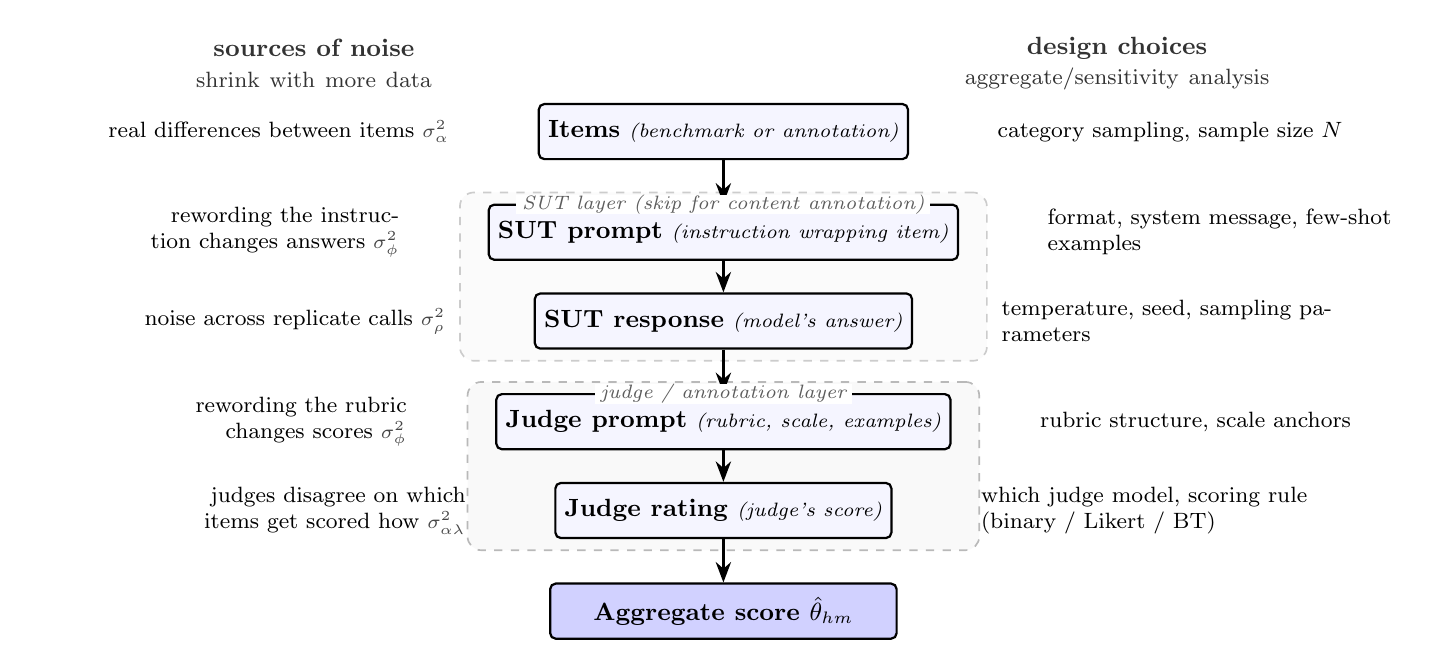
\begin{tikzpicture}[
    node distance=0.4cm and 1.6cm,
    box/.style    = {rectangle, draw, thick, rounded corners=2pt,
                     minimum width=4.0cm, minimum height=0.7cm,
                     align=center, font=\small, fill=blue!4},
    final/.style  = {box, fill=blue!18, font=\bfseries\small,
                     minimum width=4.4cm},
    layer/.style  = {draw=gray!55, dashed, semithick, rounded corners=5pt,
                     inner xsep=10pt, inner ysep=4pt, fill=gray!5},
    llabel/.style = {font=\scriptsize\itshape, text=gray!72!black,
                     fill=white, inner xsep=2pt, inner ysep=0pt},
    vleft/.style  = {font=\footnotesize, align=right, anchor=east,
                     text width=4.6cm},
    vright/.style = {font=\footnotesize, align=left,  anchor=west,
                     text width=4.6cm},
    arrow/.style  = {-{Stealth[length=2.6mm]}, thick},
    header/.style = {font=\small\bfseries, align=center,
                     text=gray!40!black, text width=4.6cm}
]

% ========= central pipeline =========
\node[box]                            (items)  {\textbf{Items} {\scriptsize\itshape(benchmark or annotation)}};
\node[box, below=0.55cm of items]     (sutpr)  {\textbf{SUT prompt} {\scriptsize\itshape(instruction wrapping item)}};
\node[box, below=of sutpr]            (sutres) {\textbf{SUT response} {\scriptsize\itshape(model's answer)}};
\node[box, below=0.55cm of sutres]    (jpr)    {\textbf{Judge prompt} {\scriptsize\itshape(rubric, scale, examples)}};
\node[box, below=of jpr]              (jres)   {\textbf{Judge rating} {\scriptsize\itshape(judge's score)}};
\node[final, below=0.55cm of jres]    (agg)    {Aggregate score $\hat{\theta}_{hm}$};

\draw[arrow] (items)  -- (sutpr);
\draw[arrow] (sutpr)  -- (sutres);
\draw[arrow] (sutres) -- (jpr);
\draw[arrow] (jpr)    -- (jres);
\draw[arrow] (jres)   -- (agg);

% ========= layer frames =========
% SUT layer drawn lighter to signal it is conditional on a benchmarking task.
\begin{scope}[on background layer]
  \node[layer, draw=gray!40, fill=gray!3,
        fit=(sutpr)(sutres)] (sutlayer) {};
  \node[layer, fit=(jpr)(jres)]      (jlayer)   {};
\end{scope}
\node[llabel, anchor=north] at ([yshift=-1pt]sutlayer.north)
   {SUT layer (skip for content annotation)};
\node[llabel, anchor=north] at ([yshift=-1pt]jlayer.north)
   {judge / annotation layer};

% ========= LEFT: random variance =========
\node[vleft] at ([xshift=-1.0cm]items.west)
    {real differences between items {\scriptsize\textcolor{gray!55!black}{$\sigma^{2}_{\alpha}$}}};
\node[vleft] at ([xshift=-1.0cm]sutpr.west)
    {rewording the instruction changes answers {\scriptsize\textcolor{gray!55!black}{$\sigma^{2}_{\phi}$}}};
\node[vleft] at ([xshift=-1.0cm]sutres.west)
    {noise across replicate calls {\scriptsize\textcolor{gray!55!black}{$\sigma^{2}_{\rho}$}}};
\node[vleft] at ([xshift=-1.0cm]jpr.west)
    {rewording the rubric changes scores {\scriptsize\textcolor{gray!55!black}{$\sigma^{2}_{\phi}$}}};
\node[vleft] at ([xshift=-1.0cm]jres.west)
    {judges disagree on which items get scored how {\scriptsize\textcolor{gray!55!black}{$\sigma^{2}_{\alpha\lambda}$}}};

% ========= RIGHT: design choices =========
\node[vright] at ([xshift=1.0cm]items.east)
    {category sampling, sample size $N$};
\node[vright] at ([xshift=1.0cm]sutpr.east)
    {format, system message, few-shot examples};
\node[vright] at ([xshift=1.0cm]sutres.east)
    {temperature, seed, sampling parameters};
\node[vright] at ([xshift=1.0cm]jpr.east)
    {rubric structure, scale anchors};
\node[vright] at ([xshift=1.0cm]jres.east)
    {which judge model, scoring rule (binary / Likert / BT)};

% ========= column headers =========
\node[header] at ([xshift=-5.2cm,yshift=0.5cm]items.north)
    {sources of noise\\{\normalfont\footnotesize shrink with more data}};
\node[header] at ([xshift=5cm,yshift=0.5cm]items.north)
    {design choices\\{\normalfont\footnotesize aggregate/sensitivity analysis}};
\end{tikzpicture}}%

\caption{TEE separates aggregation-reducible noise from design-choice sensitivity at every pipeline stage. %Each variance component on the left shrinks with more items, prompts, or replications within a chosen design. Each design choice on the right is fixed within a design but its contribution shrinks across designs (averaging over multiple judges, temperatures, or scoring rules); when no aggregation occurs, the contribution should be reported as sensitivity. 
For content-annotation tasks (e.g., labeling social media posts) the SUT layer is omitted.}
\label{fig:pipeline}
\end{figure}
% \clearpage


Figure~\ref{fig:safety_combined}(a) illustrates the TEE decomposition based on 141 safety items from the AILuminate benchmark. The 3-judge panel contributes 43.8\% of the variance with item$\times$judge adding another 16.7\%. On the other hand, prompt wording contributes less than 0.5\%. This means investing in additional judges will lower the variance more than prompts or additional benchmark items.

\subsection{Data-Generating Process}
\label{sec:dgp}

An LLM evaluation pipeline yields output $Y_{ivhm}^{(r)}$, based on item $i$ ($i = 1, \ldots, N$), prompt variant $v$ ($v = 1, \ldots, V$), temperature $h$, model $m$ (a judge or SUT), and replication $r$. Replications are repeated model calls.\footnote{In G-theory terms, these factors and the scoring protocol comprise the admissible observations.} The framework specifies the linear mixed model:

\begin{equation}
\label{eq:dgp}
\begin{split}
Y_{ivhm}^{(r)} = \mu + \alpha_i + \phi_v + \tau_h + \lambda_m 
 + (\alpha\phi)_{iv} + (\alpha\tau)_{ih} + (\phi\tau)_{vh} 
 + (\alpha\lambda)_{im} + (\phi\lambda)_{vm} \\
 + \epsilon_{ivhm} + \rho_{ivhm}^{(r)}
\end{split}
\end{equation}

where $\mu$ is the grand mean, $\alpha_i$ is the item random effect, $\phi_v$ the prompt variant random effect, $\tau_h$ the temperature fixed effect, $\lambda_m$ the model fixed effect, and the five parenthesized interaction terms are two-way interaction random effects. $\epsilon_{ivhm} \sim N(0, \sigma^2_\epsilon)$ captures cell-level error from unmodeled higher-order interactions, and $\rho_{ivhm}^{(r)} \sim N(0, \sigma^2_\rho)$ captures within-cell replicate noise. %$\epsilon_{ivhm}$ is constant within a cell, $\rho_{ivhm}^{(r)}$ varies by replication within a cell. %The cell-level term $\sigma^2_\epsilon$ does not shrink with replications $R$; only items, prompts, judges, and other facets indexing the cell can reduce it.

We treat items and prompt variants as \emph{random} to get an estimand over all items and prompts that might have been drawn. On the other hand, we treat temperature and model as \emph{fixed} because usually we select judge models with intent and generally do not seek to generalize to some model population. Similarly we consider temperatures as analogous to a ``dose'' rather than something to be sampled. Note that temperature has nonlinear, non-additive effects on output variance \citep{renze2024temperature, li2025hotcold} (SI Appendix, Section~\ref{si:temperature}). %Some LLM-as-judge applications may want to characterize variance across a population of judge models, for example to bound how rankings shift under arbitrary judge swap. We still treat model as fixed because exchangeability across typical judge panels is implausible (different model families, sizes, training distributions) and 3 - 4 judges is too few to estimate a between-model variance with usable precision; the design-sensitivity index instead summarizes spread across the specific chosen levels. 
% Averaging over an $M$-judge panel reduces the model contribution to the grand mean as $\sigma^2_\lambda/M$ (Eq.~\ref{eq:dstudy_multi}), which the empirical demonstrations rely on. 

\subsection{Variance Decomposition}
\label{sec:gstudy}

Decomposing the variance requires three formal assumptions: conditional exchangeability of replications and prompt variants, additivity with two-way interactions, and independent zero mean random effects (SI Appendix, Section~\ref{si:framework}). %Monte Carlo simulations show D-study projections remain within 8\% relative bias under four misspecification scenarios (SI Appendix, Section~\ref{si:simulations}).

For prompt variants, the exchangeability assumption requires that variants all measure the same construct. Drawing on G-theory \citep{cronbach1972dependability, brennan2001gtheory}, survey methodology on question wording \citep{groves2010survey}, and multi-prompt LLM evaluation \citep{mizrahi2024multiprompt, sclar2024sensitivity, barrie2024pss}, we require that variants hold constant the task or rubric, inserted benchmark content, answer format, reasoning level, and scoring mode (SI Appendix, Section~\ref{si:prompt_admissibility}).
%A deterministic check rejects variants that drop an input or the answer-format instruction, and an independent model not used as a judge rejects candidates it rates below 4 out of 5 for measuring the same construct. Widening the admissible set raises the MMLU prompt share of per-observation variance from 2.1\% under strict paraphrase to 20.6\% under a broader hand-authored set, so we do not claim coverage saturation. The safety share stays at 1.3\% across sets of increasing breadth (SI Appendix, Section~\ref{si:prompt_admissibility}).
%The scoring protocol also belongs to the measurement design. Components change between Likert and pairwise scoring and between the probability and logit scales (SI Appendix, Sections~\ref{si:scoring_comparison} and~\ref{si:glmm}).

Because the random effects are mutually independent, their variances add. At fixed temperature $h$ and model $m$, $\tau_h$ and $\lambda_m$ are constants and drop out, so the observation-level variance decomposes as:
\begin{equation}
\label{eq:tle}
\begin{split}
\Var(Y \mid h, m) = \sigma^2_\alpha + \sigma^2_\phi + \sigma^2_{\alpha\phi} + \sigma^2_{\alpha\tau} \\
+ \sigma^2_{\phi\tau} + \sigma^2_{\alpha\lambda} + \sigma^2_{\phi\lambda} + \sigma^2_\epsilon + \sigma^2_\rho
\end{split}
\end{equation}

At any fixed level, the temperature and model interaction terms still vary across the sampled items and prompts, so they remain in the decomposition.

%When averaging over $M$ models, a design-sensitivity term $\sigma^2_\lambda = \frac{1}{M}\sum_m(\lambda_m - \bar{\lambda})^2$ is added. The same is true for averaging over multiple temperatures. The compact DGP omits fixed-factor interactions such as temperature$\times$model. If crossed fixed factors interact substantively, the D-study adds the corresponding finite sensitivity term, for example $\sigma^2_{\tau\lambda}/(HM)$ when averaging over both temperature and model.

Random components (item, prompt variant, replication) shrink by aggregation within a chosen design; fixed-effect contributions (temperature, model, scoring method) shrink only by aggregating across designs, and otherwise should be reported as sensitivity alongside the point estimate \citep{steegen2016multiverse}.

\subsection{D-Study Projections}
\label{sec:dstudy}

Once variance components are estimated, a D-study projects the variance of the estimated grand mean $\hat{\theta}$ under a proposed design. We denote the \emph{proposed} D-study design ($N'$, $V'$, $R'$), while the observed G-study counts remain $N$, $V$, $R$, which are used to estimate the variance components. %Each variance component is divided by its number of levels, e.g., judge variance is divided by $M$ judges, cell-level error by $N'V'M$, replicate noise by $N'V'MR'$, and each interaction term by the product of its component factors. 

 In classical psychometrics with human raters, D-studies involve trying to choose how many raters, items, and occasions a study can afford \citep{brennan2001gtheory}. However, in LLM/autorater pipelines how much of each facet (e.g., $N'$ items, $V'$ variants, $R'$ replicates) a study can afford is a matter of API calls, so an autorater D-study can trade off all facets under a given compute budget.

% When the estimation design crosses $M$ models, $\sigma^2_{\alpha\lambda}$ and $\sigma^2_{\phi\lambda}$ are separately identifiable and enter the formula; in a single-model design they are absorbed into $\sigma^2_\alpha$ and $\sigma^2_\phi$ (SI Appendix, Section~\ref{si:framework}).\footnote{When items belong to categories (as in the empirical demonstrations), $\sigma^2_\alpha = \sigma^2_\kappa + \sigma^2_\delta$ combines between-category and within-category variance. If categories are themselves sampled from a larger population, the D-study formula gains a $\sigma^2_\kappa / C$ term; in the demonstrations here, categories are fixed (specific hazard types, ideology dimensions, MMLU subjects), so $\sigma^2_\kappa$ is absorbed into $\sigma^2_\alpha / N'$.} 

%When averaging over $M$ models, a design-sensitivity term $\sigma^2_\lambda = \frac{1}{M}\sum_m(\lambda_m - \bar{\lambda})^2$ is added. The same is true for averaging over multiple temperatures. With $\bar{\sigma}^2_\epsilon = \frac{1}{M}\sum_m \sigma^2_{\epsilon,m}$ and $\bar{\sigma}^2_\rho = \frac{1}{M}\sum_m \sigma^2_{\rho,m}$ denoting the cell-level and replicate-noise variances averaged over models, under a design with $N'$ items, $V'$ prompt variants, and $R'$ replications at fixed temperature:
For $N'$ items, $V'$ prompt variants, and $R'$ replications at fixed temperature, the variance is:\footnote{When averaging over $M$ models, a design-sensitivity term $\sigma^2_\lambda = \frac{1}{M}\sum_m(\lambda_m - \bar{\lambda})^2$ is added. The same is true for averaging over multiple temperatures. Here $\bar{\sigma}^2_\epsilon = \frac{1}{M}\sum_m \sigma^2_{\epsilon,m}$ and $\bar{\sigma}^2_\rho = \frac{1}{M}\sum_m \sigma^2_{\rho,m}$ are the cell-level and replicate-noise variances averaged over models.}
\begin{equation}
\label{eq:dstudy_multi}
\begin{split}
\Var(\hat{\theta}_h) = \frac{\sigma^2_\alpha}{N'} + \frac{\sigma^2_\phi}{V'} + \frac{\sigma^2_\lambda}{M} + \frac{\sigma^2_{\alpha\phi}}{N'V'} + \frac{\sigma^2_{\alpha\tau}}{N'} + \frac{\sigma^2_{\phi\tau}}{V'} \\
+ \frac{\sigma^2_{\alpha\lambda}}{N'M} + \frac{\sigma^2_{\phi\lambda}}{V'M} + \frac{\bar{\sigma}^2_\epsilon}{N'V'M} + \frac{\bar{\sigma}^2_\rho}{N'V'MR'}
\end{split}
\end{equation}

D-study variance allows us to estimate the standard error and 95\% CI: $\hat{\theta} \pm 1.96 \cdot \sqrt{\Var(\hat{\theta})}$, which accounts for all identified pipeline variance. The interval includes variance for generalizing to new judges and temperatures, which is why when the target is a fixed panel our approach is overly conservative (99 - 100\% coverage in SI Appendix, Section~\ref{si:underestimation_sim}, see also Section~\ref{si:underestimation_redraw}). 

Monte Carlo simulations (1,000 replicates) confirm that D-study intervention \emph{rankings} are highly reliable; under the default DGP, the correct top-1 intervention is identified in 98\% of simulations. Four assumption violations and a latent-ambiguity sweep each lead to $|\text{bias}| \leq 9\%$ (SI Appendix, Sections~\ref{si:dstudy_validation} and~\ref{si:latent_ambiguity}).

We use REML \citep{jiang1996reml} via \texttt{lmer} \citep{bates2015lme4} to estimate variance via a crossed random-effects specification. We consider both temperature and the model to be fixed, with every random facet and interaction as an independent term, for example, \texttt{(1|item) + (1|prompt\_variant) + (1|item:model)}. The value of variance of each of these terms corresponds to $\sigma^2$ in Equation~\ref{eq:tle}, which Equation~\ref{eq:dstudy_multi} divides by the number of levels a proposed design averages over. The full formula and pilot-design thresholds are in SI Appendix, Sections~\ref{si:framework} and~\ref{si:checklist}.

\paragraph{Choosing facets and judges.}
In practice, crossing through all possible factors rapidly becomes combinatorially expensive. We recommend running a small pilot study across the actual factors that vary in deployment and estimating the decomposition based on this to identify where the variance lies. In our applications, one or two factors usually accounted for most of the variance (most often judge choice), whereas temperature and further replications were much less important. Sampling parameters such as top-$p$ or top-$k$ could be included in the same fashion as temperature. On the other hand, switching between direct and chain-of-thought prompting, output format, or reasoning mode should be done with care since such modifications may change answer parsing or even construct of interest and thus cannot be used without passing the construct equivalence test discussed above, they are better treated as separate design factors. When selecting judges, we recommend starting with a small crossed pilot study using a broad set of plausible models, examining the judge marginals and leave-one-judge-out diagnostics (Section~\ref{sec:safety}), and comparing with human calibration labels if any. Since the recommendations depend on which prompts and judges are included in the pilot study, TEE is best applied as a diagnostic tool rather than a mechanical rule.


\section{Empirical Demonstrations}
\label{sec:empirical}

We apply the TEE decomposition across three empirical domains in the main text: binary safety classification (AILuminate), multiple-choice QA (MMLU), and pairwise model comparison validated against human votes (Chatbot Arena). For the safety and Arena demonstrations, we decompose variance across judges, treating each (prompt, SUT-response) pair as an item,\footnote{In Arena, each item is one battle, consisting of the user prompt and the two SUT responses being compared.} while in MMLU there is no judge, each benchmark question is an item, and we decompose variance across SUTs scored against the answer key (SI Appendix, Section~\ref{si:framework}). Section~\ref{sec:gaming} then quantifies the gaming surface single-configuration benchmarks expose. In the SI, we provide a political affinity annotation demonstration (Section~\ref{sec:propaganda}) with a 9-annotator human baseline, a Likert vs pairwise scoring comparison (Section~\ref{si:scoring_comparison}), and a pilot validation showing that a small sample recovers the qualitative D-study guidance of an 8$\times$ larger full run (Section~\ref{si:pilot}).

\subsection{Safety: Judge Disagreement Dominates}
\label{sec:safety}

We first illustrate the variance decomposition using AILuminate~v1.0 \citep{ghosh2025ailuminate}, a safety benchmark from MLCommons. The benchmark assesses whether LLM responses cross safety lines across 12 hazard categories (hate speech, self-harm, violent crime, etc.). Most items are unambiguously safe (94\% safe rate) and the variance concentrates on the 6\% of borderline cases where judges disagree about whether a refusal is adequate. We decompose the variance based on 36 demonstration prompts, using responses from Claude Opus 4.5, GPT-5.1, DeepSeek Chat~v3.1, and Grok 4.1 Fast (141 items after dropping 3 SUT refusals).%\footnote{We model the binary outcome with a linear probability model \citep[LPM;][]{angristpischke2009} because D-study projection formulas require linear variance components.}

Judge choice matters for safety rating variability and for item-level variance. The decomposition (Figure~\ref{fig:safety_combined}(a)) shows that the judge panel accounts for the largest share of variance (43.8\%), with the item$\times$judge interaction adding another 16.7\%. Both shrink as $1/M$ when the projection averages over $M$ judges. 

We also ran leave-one-judge-out estimates, which confirm that no one judge drives this pattern.  The three judge-related terms account for 73\% of the variance with the full panel, and 68 - 83\% after dropping any one judge (see also SI~\ref{si:lojo}). Of course, knowing \emph{which} judge is most accurate requires validation against gold standard labels (e.g., known-answer items, the hazard taxonomy, human labelled data). However, we can still get a lot of mileage from the decomposition alone --- a large judge mean offset implies we should recalibrate or remove a rater, while large item$\times$judge disagreement suggests closer review of specific cases.

\begin{figure}[htbp]
\centering
\begin{minipage}[t]{0.49\linewidth}
  \centering
  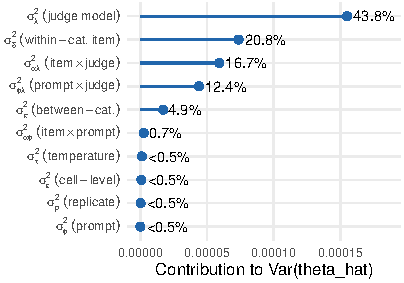
\includegraphics[width=\linewidth]{fig_intro_safety_decomposition.pdf}\\
  \footnotesize (a) Variance decomposition
\end{minipage}\hfill
\begin{minipage}[t]{0.49\linewidth}
  \centering
  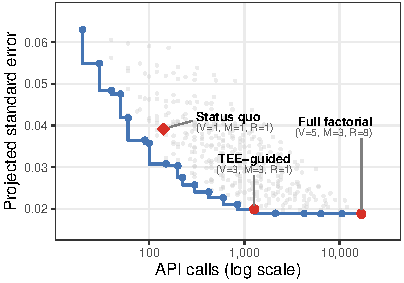
\includegraphics[width=\linewidth]{fig_cost_efficiency.pdf}\\
  \footnotesize (b) Cost-efficiency frontier
\end{minipage}
\caption{Safety decomposition (a) and cost-efficiency frontier (b) for AILuminate. Judge-model variance dominates the decomposition in (a). A TEE-guided design that aggregates over diverse judges captures most of the available SE reduction at modest cost (b).}
\label{fig:safety_combined}
\end{figure}


Within-category item heterogeneity contributes 20.8\% and prompt$\times$judge 12.4\%, with each remaining component below 5\%. Replicate noise $\sigma^2_\rho$ and cell-level error $\sigma^2_\epsilon$ are large components at the item level, but enter $\Var(\hat\theta)$ divided by $N'V'H'M'R'$ and $N'V'H'M'$ respectively, so each contributes less than 0.5\% to the variance of the mean. Per-category variance spans more than an order of magnitude in replicate noise $\hat{\sigma}^2_\rho$, from $\hat{\sigma}^2_\rho = 0.001$ for specialized advice to $\hat{\sigma}^2_\rho = 0.033$ for sex crimes (SI Appendix, Section~\ref{si:pilot}).
Temperature and prompt main effects contribute negligibly. \footnote{Three-way interaction terms (item$\times$prompt$\times$temperature, item$\times$temperature$\times$judge) are statistically significant but substantively negligible, supporting the two-way interaction specification.} 

%This is the across-design mode of aggregation introduced in Section~\ref{sec:framework}: judge model is treated as fixed in the DGP, but its contribution to the grand mean still shrinks when the design crosses multiple judges.

The D-study then projects precision under any proposed design (any new combination of $N'V'H'M'R'$, etc.), enabling a cost-efficiency analysis. Figure~\ref{fig:safety_combined}(b) plots projected standard error against API cost for 360 candidate designs of the safety benchmark. The status quo design (141 items, one prompt, one judge, no replication) sits well above the efficient frontier; for the same budget, designs on the frontier that trade some items for judge diversity reduce the SE by 9\%. A TEE-guided design (141 items, 3 prompts, 3 judges, no replication) lowers the SE by 49\% at 9$\times$ the cost, whereas running the full factorial (5 prompts, 3 judges, 8 replications) yields only an extra 5\% reduction at 120$\times$ the cost. Beyond roughly 1,000 API calls, the curve flattens out with clear diminishing returns.



\subsection{MMLU: Item and Prompt Reallocation Roughly Halves Error}
\label{sec:mmlu}

Unlike our safety analysis, which centers on an LLM-as-judge/autorater layer, our MMLU benchmark analysis has no judge model at all. Because MMLU (Massive Multitask Language Understanding) \citep{hendrycks2021mmlu} has the true answers to multiple choice problems, we have an evaluation criterion where we can measure estimation accuracy as well as coverage probability of confidence interval with respect to the answer key. In this case, the evaluation is treated as a budget-allocation problem in which, given a fixed total budget for call, the problem is how to allocate the calls among number of items ($N$), prompt variants ($V$), and replications ($R$). Three methods of comparison were applied based on the MMLU pool of 200 items: (i) a \emph{naive} allocation ($V\!=\!1$, $R\!=\!3$) where each call is repeated three times, (ii) a \emph{standard} allocation ($V\!=\!1$, $R\!=\!1$) where replication is not used in order to sample more items, and (iii) an allocation guided by TEE and uses the D-study to choose between adding items, prompts, or replications at each budget level (see SI Appendix, Section~\ref{si:mmlu} for details).

For the G-study (Figure~\ref{fig:mmlu_combined}(a)), heterogeneity of the items explains the majority of variance, with the contribution of heterogeneity within categories being 72.2\% of $\Var(\hat{\theta})$ and heterogeneity between categories contributing 7.7\%. Item$\times$SUT adds 10.5\% and SUT-model design sensitivity adds 6.7\%. By comparison, the three prompt variables combined explain only 2.7\%, with accuracy levels ranging from 83.9\% to 85.3\% across the four prompt variants.\footnote{A fifth prompt variant omitted the instruction to answer with a letter, and under an 8-token cap many responses were cut off before naming an option. Because it fails the answer-format requirement in Section~\ref{sec:gstudy}, we exclude it here; scoring its cut-off responses as wrong would increase the prompt-related share to 70\% of $\Var(\hat{\theta})$ (SI Appendix, Section~\ref{si:mmlu_parsing}).} Re-estimating the model with a logit link similarly finds item heterogeneity to be the largest component (71.4\%, with prompt terms at 6.1\%; SI Appendix, Section~\ref{si:glmm}).

Using these figures, the TEE D-study begins with sampling more items (80\% of variance) before moving on to sampling prompts (after using the 170 items left after a pilot of 30 items). Since the naive sampling approach uses two-thirds of its trials for replicating with hardly any information gain, it is 1.6 to 2.4 times more error-prone than TEE regardless of the budget size (Figure~\ref{fig:mmlu_combined}(b)). The standard strategy samples as much as items as it can; however, once all available items are sampled, its error remains unchanged. However, since TEE averages across prompt variants once the item pool is exhausted, it continues to lower its error until it achieves half of the error of the standard strategy's RMSE at larger budgets. It also yields well-calibrated confidence intervals, maintaining $\geq$97\% coverage throughout, whereas the naive CI omits prompt sensitivity and under-covers at the two smallest budgets (91\% and 93\%).

\begin{figure}[htbp]
\centering
\begin{minipage}[t]{0.49\linewidth}
  \centering
  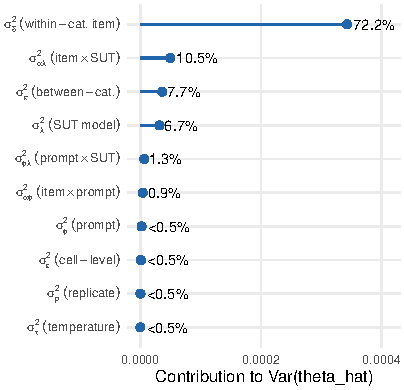
\includegraphics[width=\linewidth]{fig_mmlu_decomposition.pdf}\\
  \footnotesize (a) G-study: variance decomposition
\end{minipage}\hfill
\begin{minipage}[t]{0.49\linewidth}
  \centering
  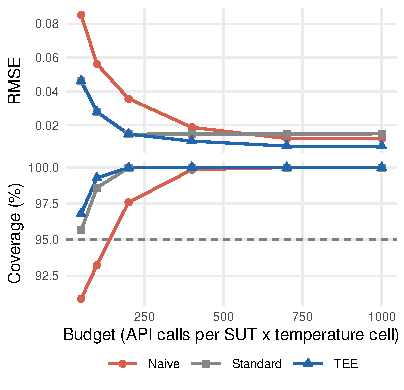
\includegraphics[width=\linewidth]{fig_budget_allocation_stacked.pdf}\\
  \footnotesize (b) D-study: budget allocation
\end{minipage}
\caption{TEE-guided estimation on MMLU roughly halves the standard RMSE at large budgets and maintains nominal 95\% CI coverage, while naive under-covers at the smallest budgets. (a)~Variance decomposition at the operational design ($N{=}200$, $V{=}4$, $M{=}3$ SUTs, $H{=}3$, $R{=}8$). (b)~RMSE against ground-truth accuracy (top) and 95\% CI coverage (bottom) by API call budget. 1,000 Monte Carlo replicates per SUT$\times$temperature cell.}
\label{fig:mmlu_combined}
\end{figure}


\subsection{Chatbot Arena: Coverage, Accuracy, D-Study Validation}
\label{sec:arena}

Chatbot Arena \citep{chiang2024chatbot} extends the domain to pairwise human choices. Gathering votes from people is slow and expensive, and (outside of Chatbot Arena) LLM judges are often used to score benchmarks. However, if we want to replace human raters with LLM judges, their scores shouldn't depend on prompt wording, judge models, etc. Thus we compare a TEE pipeline and a naïve single-judge approach with respect to 4,676 Arena matches (battles) selected from the publicly available \texttt{lmarena-ai/arena-human-preference-100k} dataset. We stratify by model and category (Creative Writing, Coding, Factual QA, and Persuasion). Each match has five prompt variants scored by three judges. We use both 1 - 5 Likert and pairwise scoring formats (see SI Section~\ref{si:arena} for details).

A simulation experiment shows that TEE averaging recovers properly calibrated uncertainty estimates. Naive 95\% CIs based on a single (judge, prompt variant) cell have reasonable coverage at $n_m = 100$, but by $n_m = 2,000$ coverage drops to 78\% (Figure~\ref{fig:arena_coverage}).  The TEE CI remains at or above 95\%. Increasing the value of $n_m$ leads to a narrower interval centered on the average of one configuration, so more data actually means worse coverage.

\begin{figure}[H]
\centering
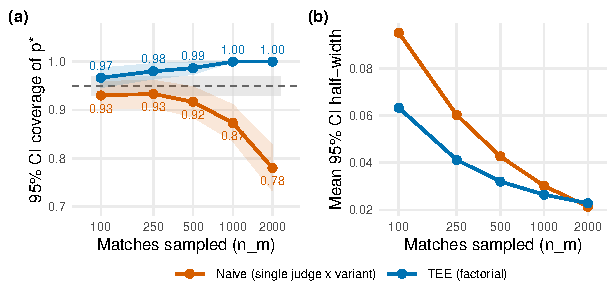
\includegraphics[width=0.75\linewidth]{fig_arena_coverage.pdf}
\caption{Naive coverage on Chatbot Arena drops as the sample grows, while TEE maintains nominal coverage. (a)~Coverage versus match sample size $n_m$ for naive and TEE. (b)~Half-width of CI versus $n_m$. TEE approaches the appropriate floor ($\sigma_V^2/V + \sigma_J^2/J$) while naive keeps shrinking. Ground truth $p^* = 0.389$ is the mean across all 3 judges and 5 prompt variants in the Likert factorial, a finite-panel target. The TEE interval instead includes variance for generalizing to new prompts and judges, so it over-covers $p^*$ at large $n_m$. An interval for the finite-panel target would hold variants and judges fixed and bootstrap over matches.}
\label{fig:arena_coverage}
\end{figure}

TEE averaging also improves per-match agreement with the individual human vote across all four categories (SI Appendix, Figure~\ref{fig:arena_accuracy}). Pooled across 4,676 matches, TEE Likert raises AB-only agreement over single-judge Likert by $+7.9$ pp (74.9\% vs.\ 67.0\%) and TEE pairwise raises it over single-judge pairwise by $+3.6$ pp (71.9\% vs.\ 68.3\%, see SI Appendix Table~\ref{tab:arena_agreement}). %Per-category lifts are positive in every cell, ranging from $+5.1$ to $+11.8$ pp for Likert and $+1.6$ to $+5.2$ pp for pairwise. %The Likert lift exceeds the pairwise lift in every category; pairwise judges almost never tie regardless of prompt wording, so the Likert-vs-pairwise comparison here is not a clean scoring-method contrast (SI Appendix, Section~\ref{si:arena}).

A D-study fit on 80\% of matches projects per-category SE reductions of 0.53 - 0.59 from single-judge to TEE. Across the four held-out categories, projected SE reductions track observed Likert agreement lifts at Spearman $\rho = 0.80$ (n = 4; SI Appendix Figure~\ref{fig:arena_dstudy_vs_observed}).

Both findings matter when the goal is to score matches one at a time, as in training supervised models on Arena labels \citep{egami2024dsl} or filtering individual items.



\subsection{Single-Configuration Benchmarks Vulnerable to Benchmark Hacking}
\label{sec:gaming}

\citet{singh2025leaderboard} document Meta running 27 private Llama-4 variants on Chatbot Arena before launch and publishing only the top scorer (\emph{benchmark hacking}), which constitutes best-of-$K$ exploitation of pipeline noise. Some ways it can happen are that, for leaderboards, many models are submitted to the leaderboard using different names, and the top performing one is reported. In open-source benchmarks, they can conduct the test inside using various forms of prompts and scoring configurations until they get a favorable score. The expected inflation is $\E[\max(Z_1,\ldots,Z_K)] \cdot \sigma_{\text{pipeline}}$, where $\sigma_{\text{pipeline}}$ is the standard deviation of the pipeline noise decomposed above. Prompt formatting alone can produce up to 76 accuracy points of spread on identical models \citep{sclar2024sensitivity}, suggesting the gameable surface is broad in practice.

We quantify the gaming surface in the context of Chatbot Arena by bootstrapping 4,676 matches across pipeline configurations (Figure~\ref{fig:gaming_surface}). The Arena human leaderboard already exposes a 45-Elo surface at $K{=}27$ from voter sampling alone, large enough to flip rankings between adjacent models. A single-configuration LLM-judge replacement ($V{=}1$, $M{=}1$) increases the surface to 56 Elo, since a developer can target both the LLM-judge configuration and the underlying voter sample. Averaging across either prompts or judges alone recovers the human baseline ($V{=}5$, $M{=}1$: 46 Elo; $V{=}1$, $M{=}3$: 46 Elo). TEE-LLM ($V{=}5$, $M{=}3$ averaging) cuts the surface to 32 Elo, about 30\% below the human leaderboard. Judge main effects account for the largest share of gameable LLM variance (Table~\ref{tab:gaming}), the component a developer most directly controls when picking judge models.

\begin{figure}[htbp]
\centering
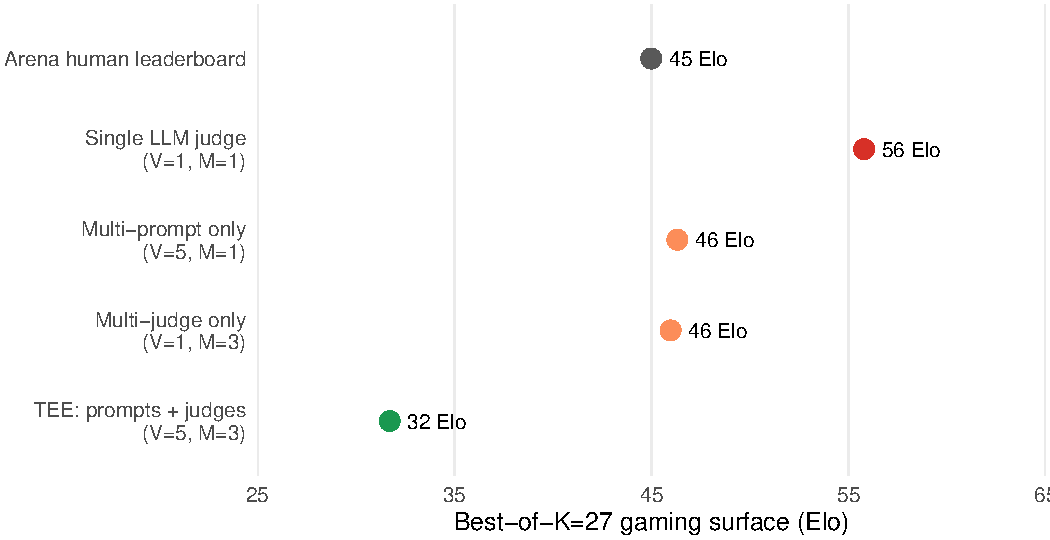
\includegraphics[width=0.8\linewidth]{fig_gaming_surface.pdf}
\caption{Best-of-$K{=}27$ gaming surface on Chatbot Arena across pipeline configurations. ``Gaming surface'' is the expected Elo boost a developer earns by submitting $K{=}27$ model variants and reporting only the highest-scoring one. Variance surface computed by bootstrapping 4,676 Arena matches.}
\label{fig:gaming_surface}
\end{figure}

The best-of-$K$ simulation comprises just one facet of the manipulation surface. \citet{singh2025leaderboard}'s analysis finds that providers can retract scores from unfavorable runs, that proprietary providers received a disproportionate share of data (61.4\% of all battle data), and that access to Arena-specific data boosted performance by up to 112\% on the Arena distribution without corresponding gains on external benchmarks.



\section{Discussion}
\label{sec:discussion}

Across the empirical demonstrations, naive error estimates substantially understate measurement uncertainty. Naive CIs omit judge disagreement, prompt sensitivity, replicate noise, and their interactions, which can lead evaluators to mistake pipeline noise for genuine benchmark capability differences or generalizable patterns in LLM-annotated research. The gap between naive and TEE-informed error estimates corresponds to the relative variance between pipelines, which scales with both subjectivity and complexity. The data we analyze from Chatbot Arena, MMLU, and our propaganda audit (SI Appendix) further show that failure to aggregate over these noise sources also reduces accuracy. %: 43.8\% of $\Var(\hat\theta)$ in safety classification, 54.4\% in Likert ideology, and 68.4\% in pairwise ideology (with an additional 20.9\% for the position factor in pairwise). MMLU removes the judge layer, and item heterogeneity (35.0\%) and SUT-model design sensitivity (25.0\%) take over. 
%Deployment decisions, safety certifications, and published findings inherit the resulting error.

 %On MMLU, where each item is exact-match verified against an answer key (no rater), naive SE underestimates the TEE-corrected SE by 57\%. On the safety benchmark, where each item is a binary safe/unsafe call against a published taxonomy and most tasks are `safe,' the underestimate is 43\%. On Likert ideology, where raters compress a multi-dimensional judgment into a 1 - 5 score, the underestimate is 60\%. Full per-domain numbers in SI Appendix, Section~\ref{si:naive_vs_tee}.
 %The gaming analysis (Section~\ref{sec:gaming}) shows further that unmeasured pipeline variance means even routine model selection inflates reported scores.

Pipeline variance can also serve as a gaming surface in benchmarking and in research. We show that submitting best-of $K{=}27$ variants (as documented in \citet{singh2025leaderboard}) inflates Chatbot Arena Elo scores by 56 points, while averaging over multiple judges and prompts cuts that surface by 43\% (\S\ref{sec:gaming}). The same vulnerability extends to LLM-annotated research, where pipeline variance maps onto labeling error and predicts misclassification against the 9-rater human consensus in our propaganda demonstration ($r = -0.68$, SI Appendix, Section~\ref{sec:propaganda}), consistent with the configuration- and adversarial-search reversals \citet{baumann2025llmhacking} document across 37 LLM-annotation tasks. The implications extend beyond model capability overestimates, as benchmarks like SWE-Bench, LegalBench, and HealthBench inform estimates of labor substitution and productivity gains \citep{eloundou2023gpts} associated with widespread LLM adoption. 


%However beyond diagnosis, accounting for the total evaluation error (TEE) tells developers how to improve estimation. A small pilot run under our TEE framework yields variance estimates (e.g., confidence intervals) that naive estimates obscure, and a ranked list of which design changes would shrink it most (SI Appendix, Section~\ref{si:pilot}).

%Chatbot Arena's human votes let us test TEE end-to-end (\S\ref{sec:arena}). Across 4,676 matches, naive coverage falls as $N$ grows while TEE-corrected coverage holds; TEE averaging lifts agreement with human votes by 7.9 points; and D-study projections fit on 80\% of matches generalize to the held-out 20\%, validating the framework against ground-truth human data.

How should researchers and benchmark designers respond in practice? Across our applications, whenever a pipeline includes an LLM judge layer, our D-study projections indicate that averaging across multiple judges reduces variance more than any other single change, followed by adding items on AILuminate and adding prompt variants on Arena. Following those projections improves both CI coverage and agreement with human ground truth. More broadly, because almost all evaluation claims aim to generalize across a domain of items, sampling more items is consistently valuable, and results should not rest on a single judge model or prompt template. Even though the variance percentages provided by the rankings here are helpful guidelines, their actual values vary depending on the application, and for this reason, doing a pilot study in the target pipeline will prove extremely useful.

Because benchmark results and LLM annotations are used to carry out safety assessments and empirical studies and make projections about the economy or labor market, underestimating the variability of the pipeline will lead to distorted conclusions further down the line. Conducting a pilot study in the TEE framework will help achieve that at much less expense than in a full factorial design.

% In naive estimation, the variance from prompts, judges, and their interactions is not averaged in pipeline variance estimates and omitted from CIs. The omission causes the under-coverage; the unaveraged variance is what a developer running best-of-$K$ exploits. The TEE-reducible share of $\sigma^2_{\text{pipeline}}$ therefore quantifies both with one number. Multi-judge multi-prompt averaging fixes both, cutting the Arena gaming surface by 43\% to below the human-leaderboard baseline.

% The rankings tend to converge on a common prescription across the demonstrations. Where a judge layer is present, averaging over judges produces the largest single variance reduction available, 37 - 45\% on AILuminate and Arena%, because $\sigma^2_\lambda/M$ and $\sigma^2_{\alpha\lambda}/(NM)$ both shrink with $M$
% . After judges, items matter most on AILuminate, prompts on Arena, and the two are comparable on MMLU (which has no judge). %Once those moves are made, additional replications buy little extra precision: they reduce $\sigma^2_\rho/(N'V'H'M'R')$, already a tiny fraction of $\Var(\hat\theta)$, but not the cell-level term $\sigma^2_\epsilon/(N'V'H'M')$, which lacks $R'$ in its denominator.

\section{Limitations}
\label{sec:limitations}


TEE has a number of simplifying assumptions worth noting. For example, when a model emits reasoning traces, the variance they generate is not attributed under the current framework and instead inflates $\sigma^2_\epsilon$. What's more, when the scoring function relies on an LLM-as-judge, its variance may compound with the SUT's \citep{haldar2025roulette, chehbouni2025neither}, and SUT$\times$judge interactions aren't currently captured in our decomposition (SI Appendix, Section~\ref{si:coverage}). 

Perhaps more importantly, TEE cannot say whether the items (eval prompts) truly cover and represent the constructs of interest, which of course limits generalizability. A toxicity benchmark that omits coded hate speech will generate precise and incomplete estimates. Total survey error has long called this coverage error \citep{sen2019tedon}.

Last, our demonstrations comprise English-only tasks with API-served models, and do not test ambiguous tasks that require open-ended reasoning. 


\section{Conclusion}
\label{sec:conclusion}

If they are provided at all, variance estimates in LLM-as-judge or autorater evaluations are anti-conservative. This means our frontier model evaluations overstate precision, while naively scored benchmarks let developers exploit measurement error in a way analogous to p-hacking or overfitting. Our TEE framework not only helps detect this issue but lets researchers estimate variance components from a small pilot study, estimate confidence intervals with valid coverage, and predict how design modifications will help in reducing error (SI Appendix, Section~\ref{si:pilot}). As LLM evaluations become more important for practical applications (model deployment, safety criteria), research, and estimates of the impact of AI on the economy and the labor market, it is vital to take pipeline uncertainty into account.

\begin{ack}
Thanks to Chris Barrie, Ben Guinaudeau, Aaron Kaufman, Brandon Stewart, Kylan Rutherford, and participants at the 2026 CSMAP conference for helpful feedback. Thanks to Peter Mattson, Bennett Hillenbrand, Andrew Gruen, Rebecca Weiss, Hannah Waight, Molly Roberts, Brandon Stewart, Eddie Yang, Ben Guinaudeau, Melina Much, Chris Barrie, Joe Higton, Kylan Rutherford, Jennifer Allen, Jonathan Nagler, and Josh Tucker for helpful early conversations about the problem of confidence intervals in LLM evals, benchmarks, and LLM-as-judge measurement problems, which helped inspire this paper.

MLCommons funded the author's salary for this work.

The author has personal financial interests in AI-related companies, in particular Nvidia, Alphabet, Microsoft, and Taiwan Semiconductor. The author worked at Facebook (now Meta) in various capacities from 2011 to 2015 and 2018 to 2020 and at Twitter (now X) from 2021 to 2023, and contracts for MLCommons, a 501(c)(6) non-profit that releases AI benchmarks, including AILuminate, which this paper analyzes (2026 to present). The author has accepted a position at Google DeepMind. For an unrelated project, the author received a 2010 Google Research Award for research on ``Social cues and reliability in content selection and evaluation.''
\end{ack}

\bibliographystyle{plainnat}
\bibliography{references}

% ----------------------------------------------------------------------
% Appendix — does not count against the 9-page limit. Phase 2 will paste
% content from paper/pnas_si_body.tex here, preserving si:* labels.
% ----------------------------------------------------------------------
\appendix
% NeurIPS appendix - migrated verbatim from paper/pnas_si_body.tex
% Section/table/figure/equation numbering is reset by \appendix in neurips_main.tex.
% All si:* labels preserved for cross-references from main text.


\section{Quickstart Guide}
\label{si:quickstart}

The steps below show how to diagnose uncertainty in an LLM annotation workflow. Section~\ref{si:framework} gives the framework and its derivation.

\begin{enumerate}\setlength{\itemsep}{6pt}
\item \textbf{Run a small pilot.} A small pilot under fixed temperature conditions may give an idea of the major sources of variance when the judge layer is manipulated. The recommended design has 30 or more items, 3 or more prompts, 2 or more judges (in case a judge layer exists), and 3 or more replications, resulting in about 540 API calls per single scoring function tested. Two prompts are the bare minimum, at the cost of less precise estimates of prompt sensitivity (Section~\ref{si:small_v}). Prompt variants have identical task instructions, output format, and reasoning mode, but might differ in terms of word usage, sentence structure, and framing of the construct (Assumption~\ref{asn:exchangeability}, Section~\ref{si:framework}). Varying the prompts this widely reflects the uncertainty that a real human evaluator would face in choosing the wording. Both paraphrasing (for example, prompting Claude Haiku at temperature 0.9 to rewrite the seed instruction in $V$ ways) and sets of a few templates varying framing of the construct are legitimate options. The latter method results in a more inclusive $\hat{\sigma}^2_\phi$. It is recommended to include the original benchmark prompt in the list of $V$ variants where available. Items should come from the target deployment domain. It is also recommended to exclude the judge facet for benchmarks without one (e.g., MMLU).

\item \textbf{Fit the variance decomposition.} The \texttt{totalevalerror} R package (\codeurl) wraps the variance decomposition, D-study, and budget-allocation routines from this paper:
\begin{verbatim}
library(totalevalerror)
des <- tee_design(pilot_df,
        outcome = score, item = item_id,
        prompt = variant_id, judge = judge_model,
        temperature = temp, replicate = rep,
        scoring = "binary")
fit <- tee_decompose(des)
\end{verbatim}
The fit reports each source of variance as a share of $\Var(\hat\theta)$, and the largest share shows where the bottleneck is. If judge variance ($\sigma^2_\lambda$) or item$\times$judge ($\sigma^2_{\alpha\lambda}$) dominates, as in the safety demonstration, adding judges helps most. If within-cell replicate noise ($\sigma^2_\rho$) dominates, add replications. If prompt sensitivity ($\sigma^2_\phi$) dominates, add prompt variants. If item heterogeneity ($\sigma^2_\alpha$) dominates, add items. The underlying fixed-temperature \texttt{lmer} formula is \texttt{score \textasciitilde{} judge + (1|item) + (1|prompt\_variant) + (1|item:prompt\_variant) + (1|item:judge) + (1|prompt\_variant:judge) + (1|item:prompt\_variant:judge)}, with the judge terms dropped for benchmarks without a judge layer. The final random effect captures cell-level idiosyncrasy; the \texttt{lmer} residual captures within-cell replicate noise. Users who prefer to fit this formula directly can do so.

\item \textbf{Optimize with the D-study.} \texttt{tee\_dstudy(fit)} gives projected SEs across alternative production designs (varying replications, prompt variants, judges, scoring methods). \texttt{tee\_budget\_allocate(fit, budget = X)} returns the cost-minimizing allocation under a fixed API budget. The projection is qualitatively reliable at pilot scale (Section~\ref{si:pilot}). The rank ordering of interventions transfers to the full design even when component magnitudes shift.

\item \textbf{Deploy and estimate CIs.} Apply the chosen production design to the full corpus, then call \texttt{tee\_se(fit)} for the corrected SE and \texttt{tee\_theta\_ci(fit, level = 0.95)} for a 95\% CI on $\hat\theta$. Because the formula incorporates the components naive CIs leave out (prompt and judge variance, plus their interactions), coverage holds near nominal even as sample size grows.

\item \textbf{Report.} \texttt{tee\_writeup(fit)} produces a paragraph summarizing the decomposition, the dominant variance components, the corrected CI, and the D-study-recommended design. For each scored measurement, also report the exact prompt text, model version, temperature, and number of replications. A tiered reporting checklist appears in Section~\ref{si:checklist}, Table~\ref{tab:checklist}.
\end{enumerate}


\clearpage

\section{Uncertainty Reporting in Current LLM Evaluation Practice}
\label{si:current_practice}

Table~\ref{tab:current_practice} surveys uncertainty reporting across thirteen widely used LLM benchmarks and annotation studies. Looking across these 13 benchmarks, most report no measurement uncertainty at all: MMLU, the Open LLM Leaderboard, MT-Bench, SWE-bench, and ARC-AGI all report only a point estimate. And the four benchmarks that do include CIs (AlpacaEval, HELM, Chatbot Arena, and Arena-Hard) only account for item-sampling variance, leaving prompt sensitivity, judge variance, temperature, and interaction terms unmeasured. Contamination in test sets occurs frequently: out of six benchmarks with publicly available test sets (MMLU, AlpacaEval, HELM, MT-Bench, Arena-Hard, and SWE-bench), training data contamination was reported in all, and even Chatbot Arena can suffer from contamination due to historical votes leaking into training data despite the live queries. In our survey, only AILuminate's private Official set and ARC-AGI held-out tasks are contaminations resistant.

The bottom row represents TEE dealing with all TEE-decomposition columns at once: prompt sensitivity, judge model and temperature, replications, interactions, item sampling, and basic CI/SE indicator. The rest of this section considers each benchmark in details.

% \begin{table}[htbp]
% \centering
% \small
% \caption{Most major benchmarks account only for single-item variance, if at all.}
% \label{tab:main_practice}
% \begin{tabular}{@{}lccccc@{}}
% \toprule
%  & Item & Prompt & Temp. & Judge & Inter. \\
% \midrule
% MMLU        & -        & - & - & n/a & - \\
% SWE-bench   & -        & - & - & n/a & - \\
% ARC-AGI     & -        & - & - & n/a & - \\
% AILuminate  & $\star$ & - & - & $^{\star}$ & - \\
% AlpacaEval     & $\star$ & - & - & - & - \\
% Chatbot Arena  & $\star$ & - & - & n/a & - \\
% \midrule
% TEE & $\star$ & $\star$ & $\star$ & $\star$ & $\star$ \\
% \bottomrule
% \end{tabular}
% \end{table}


\begin{table}[ht]
\centering
\small
\caption{Uncertainty reporting in prominent LLM evaluations. SUT-layer columns capture variance in the system under test. Judge-layer columns capture variance in the scoring pipeline.}
\label{tab:current_practice}
\resizebox{\textwidth}{!}{%
\begin{tabular}{@{}lcc ccc ccc cl@{}}
\toprule
 & & & \multicolumn{3}{c}{\textit{SUT layer}} & \multicolumn{3}{c}{\textit{Judge layer}} & & \\
\cmidrule(lr){4-6} \cmidrule(lr){7-9}
 & \rotatebox{70}{Any CI/SE} & \rotatebox{70}{Item sampling} & \rotatebox{70}{SUT prompt} & \rotatebox{70}{SUT temperature} & \rotatebox{70}{SUT replications} & \rotatebox{70}{Judge prompt} & \rotatebox{70}{Judge model} & \rotatebox{70}{Judge temperature} & \rotatebox{70}{Interactions} & \rotatebox{70}{Contamination} \\
\midrule
MMLU \citep{hendrycks2021mmlu} & - & - & - & - & - & n/a & n/a & n/a & - & High \\
Open LLM Leaderboard & - & - & - & - & - & n/a & n/a & n/a & - & Mixed \\
AlpacaEval \citep{dubois2024alpacaeval} & $\star$ & $\star$ & - & - & - & - & - & - & - & High \\
HELM \citep{liang2023helm} & $\star$ & $\star$ & - & - & - & n/a & n/a & n/a & - & High \\
Chatbot Arena \citep{chiang2024chatbot} & $\star$ & $\star$ & - & - & - & n/a & n/a & n/a & - & Medium \\
MT-Bench \citep{zheng2023llmjudge} & - & - & - & - & - & - & - & - & - & High \\
Arena-Hard \citep{li2024arenahard} & $\star$ & $\star$ & - & - & - & - & - & - & - & High \\
SWE-bench \citep{jimenez2024swebench} & - & - & - & - & - & n/a & n/a & n/a & - & High \\
ARC-AGI \citep{chollet2024arcagi} & - & - & - & - & - & n/a & n/a & n/a & - & Low \\
AILuminate \citep{ghosh2025ailuminate} & ($\star$) & - & - & - & - & - & ($\star$) & - & - & Medium \\
Gilardi et al.\ \citep{gilardi2023chatgpt} & - & - & n/a & n/a & n/a & - & - & - & - & n/a \\
T{\"o}rnberg \citep{tornberg2025llm} & - & - & n/a & n/a & n/a & - & - & - & - & n/a \\
Ziems et al.\ \citep{ziems2024css} & - & - & n/a & n/a & n/a & ($\star$) & ($\star$) & - & - & n/a \\
\midrule
\textbf{TEE} & $\star$ & $\star$ & $\star$ & $\star$ & $\star$ & $\star$ & $\star$ & $\star$ & $\star$ & n/a \\
\bottomrule
\multicolumn{11}{@{}l}{\footnotesize Deterministic scoring (exact match or test suite), no judge layer.} \\
\multicolumn{11}{@{}l}{\footnotesize Public test set with documented training-data leakage \citep{xu2024benbench}.} \\
\multicolumn{11}{@{}l}{\footnotesize Most subtests public. GPQA gated to reduce contamination.} \\
\multicolumn{11}{@{}l}{\footnotesize Human voters, not an LLM judge layer.} \\
\multicolumn{11}{@{}l}{\footnotesize Live queries, but historical votes published and prompts recur across months.} \\
\multicolumn{11}{@{}l}{\footnotesize Bootstrap CI over items, captures item sampling only.} \\
\multicolumn{11}{@{}l}{\footnotesize Public task set with documented solution leakage into training data.} \\
\multicolumn{11}{@{}l}{\footnotesize Private held-out evaluation set with human-calibrated difficulty.} \\
\multicolumn{11}{@{}l}{\footnotesize Paper specifies bounds from evaluator false-safe/false-unsafe rates. Ensemble of evaluators fixed. Public leaderboard displays grade only.} \\
\multicolumn{11}{@{}l}{\footnotesize Public DEMO subset (1,200 prompts) and public Practice set (12,000), with private Official test set (12,000).} \\
\end{tabular}%
}
\end{table}

\paragraph{MMLU and the Open LLM Leaderboard.} MMLU \citep{hendrycks2021mmlu} evaluates each model once on a fixed test set (14,079 items) with a single prompt format. Open-weight models with access to logits score according to log-likelihoods of the answer choices, while API-only models use the evaluation process of text generation and answer-letter parsing, which brings back the role of temperature and replicate noise. In both cases, no variability information is provided. The main source of missing variability is the item heterogeneity. From our 200-item factorial decomposition (SI Appendix, Section~\ref{si:mmlu}), within-category item heterogeneity accounts for 72.2\% of $\Var(\hat\theta)$, item$\times$SUT 10.5\%, between-category heterogeneity 7.7\%, and SUT-model design sensitivity 6.7\% at the operational design, while the three prompt terms together account for 2.7\%. According to \citet{sclar2024sensitivity}, the differences in formatting may yield up to 76 accuracy points variability. These formatting perturbations are different from phrasing-and-framing variations used in this paper (Assumption~\ref{asn:exchangeability}). Different implementations of MMLU (original, HELM, HuggingFace) have different prompt templates and yield different rankings of the same models \citep{alzahrani2024benchmarks}. It is also the case for the Open LLM Leaderboard. Most of its subtests use publicly available test sets, except for GPQA, where it is gated.

\paragraph{AlpacaEval.} AlpacaEval 2.0 \citep{dubois2024alpacaeval} scores model outputs on a reference set using only one LLM judge (GPT-4 Turbo) with one prompt, and calculates the standard error that captures variance due to item sampling. Every other pipeline parameter is kept constant (only one judge, one prompt, one temperature, and no replication). A different judge would lead to a different win rate; however, judge variance ($\sigma^2_\lambda$) is not estimated. The length controlled version adjusts the scoring for response length but not for pipeline parameter variance.

\paragraph{HELM.} HELM \citep{liang2023helm} assesses each model for each scenario using a fixed format of the prompt and 3 random seeds on different in-context example sets to ensure stability. All prompts, predictions, and test items are publicly available; therefore, HELM is subject to test set contamination due to data leakage during the training process \citep{xu2024benbench}. The evaluation relies on deterministic automated metrics (accuracy, BLEU, ROUGE, F1), not LLM judges, and thus there is no need to estimate judge variance. The sensitivity of the SUT to the prompt and temperature applies but is not estimated.

\paragraph{Chatbot Arena.} Chatbot Arena \citep{chiang2024chatbot} computes Bradley-Terry \citep{bradley1952rank} coefficients (labeled as Elo ratings) via maximum likelihood estimation with sandwich robust standard errors, collecting an average of roughly 8,000 votes per model. Prompt phrasing emerges organically among users but is neither controlled nor deconstructed. Voter heterogeneity (human rankings differ) and SUT temperature (fixed per model by the provider) both hold but are not separated from sampling error. Bootstrapping captures uncertainty in vote sample but not the variant-selection effects noted by \citet{singh2025leaderboard}, where dozens of private SUT variants were tried by providers, and only the top-scoring variant was made public.

\paragraph{MT-Bench.} MT-Bench \citep{zheng2023llmjudge} tests SUTs on 80 multi-turn questions (2 turns each; 8 categories) scored from 1 to 10 by GPT-4. There is no specific judge model version tied to the codebase; hence, an issue of replicability since the alias refers to changing model versions. The test uses only one prompt template per question at judge temperature 0 with no replicates and no CI. SUT temperature varies by category (from 0.0 to 0.7). According to the LMSYS team's later study of their benchmark, only 22.6\% of model pairs have non-overlapping CIs on MT-Bench versus 87.4\% on Arena-Hard \citep{li2024arenahard}; hence, the scores do not statistically discriminate most model pairs.

\paragraph{Arena-Hard.} Arena-Hard-Auto \citep{li2024arenahard} evaluates SUTs on 500 challenging user queries drawn from Chatbot Arena, scored by GPT-4-Turbo in pairwise comparison against a baseline (GPT-4-0314). The two-step position swap procedure helps mitigate bias from the placement of the model. The bootstrap confidence intervals involve 100 resamples and show variability of the sampled data without taking into account the variability of the judgment; the experiment included only one judge, one template prompt, and a temperature of 0. The Arena-Hard benchmark obtained a separation score of 87.4\%, which is the highest among automated benchmarks considered. Its test set is public.

\paragraph{SWE-bench.} The SWE-bench family \citep{jimenez2024swebench} evaluates coding agents on real GitHub issues. SWE-bench Verified (500 human-validated Python tasks) was the standard benchmark until contamination was found across all frontier models. SWE-bench Pro provides an alternative that is more difficult and less polluted: it has 1,865 tasks across 41 repositories, where each one needs at least $\geq$10 lines changes and averages 4.1 files being repaired per task. The score is deterministic as the agent's repair is applied to the repository and then validated against the test cases using Pass@1 that assesses the pass rate after the first attempt. There is no judge, and there is no confidence interval. Differences in format, temperature, and number of replications may still affect the patches.

\paragraph{ARC-AGI.} The ARC-AGI benchmark \citep{chollet2024arcagi} evaluates abstract reasoning on grid-transformation tasks across three versions of increasing difficulty: ARC-AGI-1 (2019, now largely solved with frontier models exceeding 96\%), ARC-AGI-2 (2025, where frontier models reach $\sim$77\%), and ARC-AGI-3 (2026, interactive reasoning). In the static versions (1 and 2), scoring is done through an exact match, and two chances are provided for each input. In contrast, version 3 measures behavior. Contamination is minimized using a separate set of 100 - 120 tasks for each version. Task difficulty is calibrated through human studies; more than 400 participants were involved in task calibration in version 2. ARC-AGI-2 adds another measure: cost per task. The score itself remains a single point estimate, with no confidence interval or uncertainty decomposition.

\paragraph{AILuminate.} AILuminate v1.0 \citep{ghosh2025ailuminate} evaluates SUT safety across 12 hazard categories (1,000 prompts each in the public Practice set and 12,000 in the private Official set, plus a 1,200-prompt Creative Commons DEMO subset). Scoring involves the use of an unchanging set of safety evaluator models, which indicate violations. The final scores (Poor/Fair/Good/Very Good/Excellent) depend on how many violations there are compared to a reference model. The technical paper specifies a methodology for computing upper and lower score bounds from evaluator false-safe and false-unsafe rates (uniquely among the benchmarks surveyed here), but the public leaderboard displays only the categorical grade. The methodology does not decompose factors such as item sampling, prompt sensitivity, evaluator-model selection (the ensemble is fixed), and their interactions, and the authors recognize that there is ``considerable variance in test outcomes'' because of prompt sampling and noise in the evaluator.

\paragraph{LLM-as-annotator studies.} \citet{gilardi2023chatgpt} compare ChatGPT (GPT-3.5-turbo) annotations to trained research-assistant labels on political text classification, reporting accuracy and intercoder agreement (Cohen's $\kappa$, \citealt{cohen1960kappa}). The study does vary temperature (1.0 and 0.2) and collects two responses per setting, finding 91\% intercoder agreement between two ChatGPT runs at $T = 1$ and 97\% at $T = 0.2$. Gilardi et al.\ is a methods validation paper and not a downstream analysis; therefore, the absence of pipeline-variance CIs is not by itself a problem. Subsequent annotation studies follow the same single-configuration practice: \citet{tornberg2025llm} uses GPT-4 with a single zero-shot prompt on political tweets. \citet{heseltine2024llm} compare GPT-4 expert coding across four countries with a single prompt and temperature. The guidelines for management research provided by \citet{carlson2026smj} reveal the dangers of small decisions in implementations, as these can greatly change the annotation results of LLMs and lead to changes in downstream results. The above single-configuration approach has become popular in downstream hypothesis testing, where LLM annotations act as regression variables and the pipeline variance TEE quantifies directly affects statistical conclusions \citep{baumann2025llmhacking, egami2024dsl}.



\clearpage

\section{Full Framework: Assumptions, Derivations, and Extensions}
\label{si:framework}

This section gives the formal assumptions, the variance decomposition, the two-tier classification, the heteroscedastic generalization, and our approach to estimation.

\subsection{Model Terms and Factor Classification}

Table~\ref{tab:factors} categorises the factors in the TEE data-generating process.

\begin{table}[ht]
\centering
\caption{Factors in the TEE data-generating process (DGP), categorised as fixed or random. Random factors (item, prompt variant, replication) stand for exchangeable draws from a larger populations, with their variance components reducing as they are aggregated \emph{inside a chosen design} (Tier~1). Fixed factors (temperature, model, scoring method) stands for specific researcher choices. When no aggregation happens, their sensitivity indices quantify researcher degrees of freedom (Tier~2). When the design \emph{does} cross multiple levels of a fixed factor (e.g., averaging over a panel of judges), the corresponding sensitivity contribution also reduces as $1/L$. This aggregation across designs is what the empirical sections depend upon for judge-model averaging.}
\label{tab:factors}
\small
\begin{tabular}{lllp{5.5cm}}
\toprule
\textbf{Factor} & \textbf{Type} & \textbf{Levels} & \textbf{Examples} \\
\midrule
Item $i$ & Random & $N$ (large) & A specific social media post; a safety test prompt together with the SUT response being judged \\
Category $c$ & Random grouping & $C$ & Hate speech type, hazard category \\
Prompt variant $v$ & Random & $V$ (3 - 5) & ``Is this post hateful?'' vs.\ ``Does this contain hate speech?'' \\
Temperature $h$ & Fixed & $H$ (e.g., 3) & $T = 0.0, 0.7, 1.0$ \\
Model $m$ & Fixed & Small set & GPT-4o, Claude Haiku~4.5, Gemini~2.0 Flash \\
Scoring method & Fixed (Tier 2) & Typically 1 & Exact match, Likert, LLM-as-judge \\
Replication $r$ & Random (nested) & $R$ (3 - 10) & Repeated API call with identical inputs \\
\bottomrule
\end{tabular}
\end{table}

\begin{table}[ht]
\centering
\caption{Variance components exploitable in single-configuration benchmarks (Likert decomposition of Chatbot Arena, aggregated across the four categories). Empirical shares from the full-factorial decomposition (4,676 matches, 5 prompt variants, 3 judges). Shown as proportions of per-observation variance $\sigma^2_\text{total}$ as gaming leverages single-configuration noise directly, before averaging reduces any component. ``How it inflates scores'' refers to two channels: (1)~passive inflation, where the benchmark operator's single-configuration design leaves noise that increases CIs width for all submissions, and (2)~active exploitation, where a developer who can probe the benchmark's specific configuration optimizes against it.}
\label{tab:gaming}
\small
\begin{tabular}{p{2.6cm}p{1.4cm}p{4.2cm}p{3.9cm}}
\toprule
\textbf{Variance component} & \textbf{Empirical share} & \textbf{How it inflates scores} & \textbf{Mitigation} \\
\midrule
Prompt sensitivity $\sigma^2_\phi$ & 1.2\% & \textit{Passive:} benchmark's single prompt carries unquantified phrasing noise. \textit{Active:} developer tunes output to the known prompt style & Average $\geq$3 diverse prompt variants \\
Judge model $\sigma^2_\lambda$ (fixed) & 8.8\% & \textit{Passive:} a single judge's systematic bias shifts all scores. \textit{Active:} developer optimizes for the specific judge's choices & Multi-judge average or report all judges \\
Item$\times$prompt $\sigma^2_{\alpha\phi}$ & 2.5\% & \textit{Passive:} item-specific phrasing noise inflates CIs. \textit{Active:} developer targets responses the chosen prompt phrasing scores leniently & Multi-prompt averaging \\
Item$\times$judge $\sigma^2_{\alpha\lambda}$ & 18.0\% & \textit{Passive:} a single judge's item-level idiosyncrasies inflate CIs. \textit{Active:} developer fine-tunes on items the chosen judge scores leniently & Multi-judge averaging eliminates this interaction \\
Prompt$\times$judge $\sigma^2_{\phi\lambda}$ & 0.7\% & Specific (judge, prompt) cell biases compound when both are fixed & Multi-prompt $\times$ multi-judge averaging \\
\bottomrule
\end{tabular}
\end{table}

The unit of analysis is one ``item'' (a benchmark case, social media post, or something similar) scored once at one combination of prompt variant, temperature, model, and replication. A typical pipeline involves two LLM calls, with the system under test (SUT) generating an output and a judge scoring it. The DGP is applied on a per-layer basis. At the judge layer, ``item'' is a (prompt, SUT-response) pair; at the SUT layer, ``model'' indexes SUTs and the variance components capture SUT-side properties. The default target estimand is $\theta_{hm} = \E_{i,v,r}[Y_{ivhm}^{(r)}] = \mu + \tau_h + \lambda_m$, the expected value of the scored output over exchangeable items, prompt variants, and replications, conditional on fixed design choices. TEE quantifies how much uncertainty each step of the pipeline adds to $\hat{\theta}_{hm}$.

We treat a factor as random if its levels are exchangeable and as fixed if they are not. Temperature is fixed because its levels produce different generation modes and cannot be exchanged (see Section~\ref{si:temperature}). Prompt variants are random because, under Assumption~\ref{asn:exchangeability}, we do not expect any wording or framing to be consistently better than the others, as long as all variants share the same reasoning mode and output format. Scoring method is fixed because it defines the residual distribution and relates to prompt sensitivity.

When items belong to content categories, $\alpha_i = \kappa_{c(i)} + \delta_{i|c}$, where $\kappa_c \sim N(0, \sigma^2_\kappa)$ captures between-category variance and $\delta_{i|c} \sim N(0, \sigma^2_\delta)$ captures within-category heterogeneity:
\begin{equation}
\sigma^2_\alpha = \sigma^2_\kappa + \sigma^2_\delta
\end{equation}

\subsection{Target Estimand}
\label{si:estimand}

The target estimand is the expected scored output, given the researcher's fixed choices of design (temperature $h$, model $m$):
\begin{equation}
\label{eq:estimand}
\theta_{hm} = \E_{i, v, r}\!\left[Y_{ivhm}^{(r)}\right] = \mu + \tau_h + \lambda_m
\end{equation}
where the expectation averages over random factors such as items, prompt phrasings, and replications while keeping temperature and model fixed. In generalizability theory, $\theta_{hm}$ is the ``universe score'' \citep{bayerl2007gtheory, brennan2001gtheory}. When averaging over $H$ selected temperature levels, $\theta_m = \frac{1}{H}\sum_h \theta_{hm} = \mu + \bar{\tau} + \lambda_m$ is a finite average over those chosen levels. Similar to this, a multi-judge target stands as a finite average over the selected judge panel, with $\sigma^2_\lambda$ measuring sensitivity inside that panel rather than a superpopulation variance over all possible judges.

Some benchmark reports focus only on a fixed set of available items. In this finite-benchmark case, item main effects are treated as fixed rather than sampled, so the $\sigma^2_\alpha/N'$ term does not need to appear in the D-study formula anymore. The remaining prompt, judge, temperature, interaction, cell-level, and replicate terms still capture how much the reported score is dependent on the chosen measurement pipeline for that particular item set.

TEE can be applied in three types of situations. The first situation is when the measurement is the construct itself, such as in LLM benchmarking and LLM-as-judge tasks where the scores of the generated output will determine the measurement variable. The second scenario is when the pipeline stability is a goal itself; where, despite there being no bias in the pipeline in the mean sense, the high variance of its measurements can render the pipeline outputs unusable. The third scenario is when LLM labels are used as substitutes in downstream analysis. This $\theta_{hm}$ serves as a proxy to an external ground truth $\theta^* = \E[Y^*]$, and the surrogate labeling error $\tilde{Y} - Y^*$ contributes bias and variance that is not accounted for by TEE alone. In Section~\ref{si:dsl}, we elaborate on the formal connection to the DSL framework \citep{egami2024dsl}, explaining which TEE terms correspond to components of the surrogate labeling variance.

Item heterogeneity ($\sigma^2_\alpha$) is signal added with noise. The signal represents differences in item labels that exist due to measured construct and not because of any defect in the process of measurement. A D-study recommending that we add more items to achieve higher precision (reduces $\Var(\hat\theta_{hm})$) does not help in achieving higher validity (the distance between $\theta_{hm}$ and $\theta^*$). Separating signal component of $\sigma^2_\alpha$ from the noise component needs an external anchor such as human labels, known-answer items, or a validation sample, and is not in TEE's scope.

These error bars will not be able to project outside of the population of items specified in the estimand. The error bars are also dependent on the assumption that the sampling frame has all the items of interest within it. Despite having proper error bars for TEE, incorrect estimation can still take place if some hazard categories are omitted from the item list. Section~\ref{si:coverage} discusses this boundary.

\subsection{Assumptions}

The decomposition requires the following assumptions:

\begin{assumption}[Conditional Exchangeability]
\label{asn:exchangeability}
Replications $r = 1, \ldots, R$ are exchangeable given $(i, v, h, m)$. Infrastructure nondeterminism \citep{yuan2025numerical} that varies across repeated calls is absorbed into $\rho_{ivhm}^{(r)}$; stable cell-level idiosyncrasy from omitted higher-order interactions is absorbed into $\epsilon_{ivhm}$. Similarly, prompt variants $v = 1, \ldots, V$ are exchangeable given item $i$. In other words, $\sigma^2_\phi$ captures sensitivity to both phrasing and framing within a fixed task instruction, output format, and reasoning mode. Variants share the canonical task and rubric structure but may differ in word choice, sentence structure, and the specific framing of the underlying construct. 

In the empirical demonstrations, prompt variants were authored as a small set of templates that vary framing while preserving task and output format, with the original benchmark prompt included where one exists; the propaganda demonstration also used an LLM paraphrase pipeline (\texttt{anthropic/claude-haiku-4.5}, temperature 0.9) on a seed instruction \citep{mizrahi2024multiprompt, barrie2024pss}. The safety and MMLU variants passed a deterministic format check and a construct-equivalence screen computed independently of the scores; one MMLU variant failed the format check and is excluded (Section~\ref{si:mmlu_parsing}). The Arena and propaganda variants predate the screen and were not screened. Section~\ref{si:prompt_admissibility} reports the screen, its validation against off-construct decoys, and how $\hat\sigma^2_\phi + \hat\sigma^2_{\alpha\phi}$ moves as the variant universe widens from strict paraphrase to construct reframing (flat for safety; 2.1\% to 20.6\% of G-study variance for MMLU). The reported $\hat{\sigma}^2_\phi$ is therefore an upper bound on what a strict-paraphrase design would estimate and a lower bound relative to broader framing sets or designs that also cross output format or reasoning mode; simulation confirms that D-study projections hold under exchangeability violations of this kind (Section~\ref{si:dstudy_validation}, Scenario~3).
\end{assumption}

\begin{assumption}[Additivity with Two-Way Interactions]
\label{asn:additivity}
Effects are additive up to two-way interactions. Higher-order interactions are absorbed into the residual. Monte Carlo evidence (Section~\ref{si:additivity}) shows that D-study projections tolerate three-way interactions with magnitudes up to 100\% of the largest two-way component. The restriction is testable via a likelihood ratio test.
The compact formulas also omit fixed-by-fixed interactions such as temperature$\times$model. When a design crosses multiple fixed factors, and their interaction is substantively large, add the corresponding finite sensitivity term to the D-study formula.
\end{assumption}

\begin{assumption}[Distributional Assumptions]
\label{asn:normality}
All random effects are normally distributed with mean zero and mutually independent. The normality assumption can be relaxed for REML estimation \citep{jiang1996reml}. Mutual independence is the more substantive assumption, with two violations warranting scrutiny. First, the model assumes item difficulty is independent of prompt sensitivity ($\alpha_i \perp (\alpha\phi)_{iv}$), yet ambiguous items may be more prompt-sensitive. Second, the model assumes difficulty is independent of temperature sensitivity ($\alpha_i \perp (\alpha\tau)_{ih}$), yet items near a decision boundary should be where temperature matters most. Section~\ref{si:dstudy_validation}, Scenario~2 shows that even strong dependence produces $\leq$2\% D-study bias.
The D-study formulas use pooled interaction variances across fixed levels. If item$\times$judge, item$\times$temperature, residual, or replicate variance differs sharply by fixed level, use stratum-specific variance estimates or the heteroscedastic extension; the pooled formula is inappropriate in that case.

For binary outcomes, the linear model is a linear probability model (LPM), adequate when baseline rates are moderate (0.3 - 0.7). At extreme rates, a GLMM robustness check is recommended (Section~\ref{si:glmm}).
\end{assumption}

\subsection{Variance Decomposition Derivation}

The variance of a single observation at fixed $h$ and $m$ follows from mutual independence of random effects:
\begin{equation}
\Var(Y \mid h, m) = \sigma^2_\alpha + \sigma^2_\phi + \sigma^2_{\alpha\phi} + \sigma^2_{\alpha\tau} + \sigma^2_{\phi\tau} + \sigma^2_{\alpha\lambda} + \sigma^2_{\phi\lambda} + \sigma^2_\epsilon + \sigma^2_\rho
\end{equation}

Averaging over $H$ temperatures introduces a design-sensitivity term:
\begin{equation}
\sigma^2_\tau = \frac{1}{H}\sum_{h=1}^{H}(\tau_h - \bar{\tau})^2
\end{equation}
This is computed from fixed effects, not REML, and depends entirely on which temperature levels the researcher chose. Model choice is analogous, with $\sigma^2_\lambda = \frac{1}{M}\sum_m(\lambda_m - \bar{\lambda})^2$.

The variance components divide into random-effect components, which shrink with more data, and fixed-effect sensitivity indices, which measure dependence on researcher choices. This partition maps onto the researcher degrees of freedom problem \citep{simmons2011falsepositive}, since temperature, scoring method, model, and system prompt are arbitrary choices that could have been made differently. TEE quantifies the sensitivity of $\hat{\theta}$ to each choice, analogous to the multiverse analysis of \citet{steegen2016multiverse}. Further design choices that can vary across runs include scoring or extraction method ($\sigma^2_{\text{extract}}$), system prompt ($\sigma^2_{\text{sys}}$), infrastructure ($\sigma^2_{\text{infra}}$), and temporal drift ($\sigma^2_{\text{drift}}$). \citet{barrie2025replication} catalog these. Each enters as an additional fixed factor when the design varies it.

\subsection{Per-Observation Variance Decomposition}
\label{si:per_observation}

Often, statistical work decomposes variance at the observation level rather than for an aggregate quantity of interest like $\Var(\hat{\theta})$, as we do in the main text and here in the SI. The per-observation share $\hat\sigma^2_k / \sigma^2_{\text{total}}$ characterizes the data-generating process before any averaging takes place, which makes it useful for examining the variance of individual LLM calls (for instance, Table~\ref{tab:gaming} reports per-observation shares to show the single-call variance profile, while the gaming surfaces themselves are estimated via bootstrap in Section~\ref{sec:gaming}).

When the goal is instead to report an aggregate estimate like the mean $\hat\theta$ and understand what drives its standard error, the $\Var(\hat\theta)$ share is the more relevant summary. Because each component $\hat\sigma^2_k$ enters $\Var(\hat\theta)$ divided by the number of factor levels averaged over (e.g., $\sigma^2_\alpha/N$, $\sigma^2_\lambda/M$, $\sigma^2_\rho/(NVHMR)$), a component that looks large at the single-observation level can become negligible in the variance of the mean once divided by a large denominator. In our safety application, for example, replicate noise $\sigma^2_\rho$ accounts for 21\% of per-observation variance, but less than 0.5\% of $\Var(\hat\theta)$ at $R = 8$ because it is divided by $NVHMR = 50{,}760$. Conversely, judge-model design sensitivity $\sigma^2_\lambda$ is only 0.8\% of per-observation variance, yet accounts for 43.8\% of $\Var(\hat\theta)$ because it is only divided by $M = 3$.

Both summaries come from the same REML fit: per-observation shares are useful when comparing the underlying DGP across studies, link functions, or scoring methods, whereas $\Var(\hat\theta)$ shares directly reflect the standard error of the mean under a specific design and guide budget allocation, judge averaging, and sample-size decisions.

\subsection{Estimation, Identifiability, and Diagnostics}
\label{si:estimation}

\paragraph{Estimation.} TEE uses REML via \texttt{lme4::lmer} in R. The base \texttt{lmer} call (cross-model design):
\begin{verbatim}
lmer(Y ~ temperature + model +
     (1|item) + (1|prompt_variant) +
     (1|item:prompt_variant) +
     (1|item:temperature) +
     (1|prompt_variant:temperature) +
     (1|item:model) +
     (1|prompt_variant:model) +
     (1|item:prompt_variant:model:temperature),
     data = df)
\end{verbatim}
Under category nesting, add \texttt{(1|category)}. Variance components are extracted via \texttt{VarCorr()}. Fixed-effect sensitivity indices use population variance ($1/H$, not $1/(H{-}1)$).

\paragraph{Boundary estimates.} Variance components at exactly zero (singular fits) occur routinely when the true variance is small. Report boundary estimates transparently. Bayesian alternatives with half-$t$ priors \citep{gelman2006prior} avoid boundary issues.

\paragraph{Identifiability.} The model requires a factorial design with every item evaluated under every prompt variant, at every temperature, and by every model. The recommended design uses $N \geq 30$ items, $V \geq 3$ prompt variants, and $R \geq 3$ replications, and $V = 2$ is the bare minimum. Prompt sensitivity ($\sigma^2_\phi$) is the hardest to estimate precisely. For $\sigma^2_\phi > 0$, moving from $V = 2$ to $V = 3$ cuts RMSE by about a third in simulation (Section~\ref{si:small_v}).

\paragraph{Diagnostics.} (1)~QQ plots of BLUPs \citep[best linear unbiased predictions;][]{robinson1991blup} for normality. (2)~Residual-vs-fitted plots for heteroscedasticity. (3)~Three-way interaction test via likelihood ratio. (4)~BLUP magnitude vs.\ item difficulty for independence violations. (5)~Category-level interaction decomposition.

\subsection{Heteroscedastic Extension}
\label{si:heteroscedastic}

The base model assumes common $\sigma^2_\epsilon$ and $\sigma^2_\rho$ across temperatures. In practice, greedy decoding and sampled decoding can produce different cell-level and replicate-level variances. The heteroscedastic extension replaces the common terms with $\epsilon_{ivhm} \sim N(0, \sigma^2_{\epsilon,h})$ and $\rho_{ivhm}^{(r)} \sim N(0, \sigma^2_{\rho,h})$. We can estimate these variances with per-stratum REML in \texttt{lme4::lmer} (near-zero bias, $<$0.3\%) or with \texttt{nlme::lme()} \citep{pinheirobates2000} and \texttt{weights = varIdent}.

\subsection{D-Study Formulas: Full Derivation}

For a single model at fixed temperature, the projected variance of $\hat{\theta}_{hm}$ is
\begin{equation}
\Var(\hat{\theta}_{hm}) = \frac{\sigma^2_\alpha}{N'} + \frac{\sigma^2_\phi}{V'} + \frac{\sigma^2_{\alpha\phi}}{N'V'} + \frac{\sigma^2_{\alpha\tau}}{N'} + \frac{\sigma^2_{\phi\tau}}{V'} + \frac{\sigma^2_{\epsilon,h}}{N'V'} + \frac{\sigma^2_{\rho,h}}{N'V'R'}.
\end{equation}
Under category nesting, $\sigma^2_\alpha \to \sigma^2_\delta$ plus a $\sigma^2_\kappa/C'$ term, where $C'$ is the number of categories in the projected design. Averaging over $H$ temperatures gives
\begin{equation}
\Var(\hat{\theta}_m) = \frac{\sigma^2_\alpha}{N'} + \frac{\sigma^2_\phi}{V'} + \frac{\sigma^2_\tau}{H} + \frac{\sigma^2_{\alpha\phi}}{N'V'} + \frac{\sigma^2_{\alpha\tau}}{N'H} + \frac{\sigma^2_{\phi\tau}}{V'H} + \frac{\bar{\sigma}^2_\epsilon}{N'V'H} + \frac{\bar{\sigma}^2_\rho}{N'V'HR'}.
\end{equation}
Projecting across $M$ models at fixed temperature adds the model-related interaction terms,
\begin{equation}
\Var(\hat{\theta}_h) = \frac{\sigma^2_\alpha}{N'} + \frac{\sigma^2_\phi}{V'} + \frac{\sigma^2_\lambda}{M} + \frac{\sigma^2_{\alpha\phi}}{N'V'} + \frac{\sigma^2_{\alpha\tau}}{N'} + \frac{\sigma^2_{\phi\tau}}{V'} + \frac{\sigma^2_{\alpha\lambda}}{N'M} + \frac{\sigma^2_{\phi\lambda}}{V'M} + \frac{\bar{\sigma}^2_\epsilon}{N'V'M} + \frac{\bar{\sigma}^2_\rho}{N'V'MR'}.
\end{equation}
All three formulas follow from the expected mean squares (EMS) of the mixed design \citep[ch.~9]{brennan2001gtheory}. The EMS table appears in Section~\ref{si:gtheory}.
When averaging jointly over temperature and model, add the finite main-effect terms $\sigma^2_\tau/H$ and $\sigma^2_\lambda/M$. If their fixed-factor interaction is non-negligible, add $\sigma^2_{\tau\lambda}/(HM)$.

The safety classification design from Section~\ref{sec:safety} shows how these formulas convert real variance estimates into a confidence interval and which design changes they flag as high-leverage. The factorial covers $N = 141$ items spanning $C = 12$ hazard categories, with $V = 5$ prompt variants, $H = 3$ temperatures, $M = 3$ judge models, and $R = 8$ replications per cell. Variance components estimated on this design reveal that judge-model design sensitivity dominates at 43.8\% of $\Var(\hat\theta)$, item$\times$judge interaction adds 16.7\%, and prompt$\times$judge another 12.4\%. The three judge-related components together account for roughly 73\% of the variance budget. Within-category item heterogeneity contributes 20.8\%, and the remaining components each fall below 5\%. Plugging these into the multi-model formula yields $\Var(\hat\theta) = 0.000354$, $\text{SE}(\hat\theta) = 0.019$, and a 95\% CI of $0.942 \pm 0.037$ for the overall safe rate. The same formula reveals which design changes would shrink that variance further. Adding 5 replications above the existing 8 improves $\Var(\hat\theta)$ by less than 0.1\% because $\sigma^2_\rho/(NVHMR)$ is already a tiny share of the variance budget once divided by all four other factors. Committing to a single judge model inflates $\Var(\hat\theta)$ by 106\% because $\sigma^2_\lambda$ loses its $1/M$ averaging benefit. The dominance pattern and the counterfactuals point the same way, so the D-study directs additional spend toward more judges and items.



\subsection{Comparison with Concurrent Frameworks}
\label{si:comparison}

Table~\ref{tab:comparison} compares TEE with concurrent variance decomposition and uncertainty quantification frameworks for LLM evaluation.

\begin{table}[ht]
\centering
\caption{Feature comparison of TEE with concurrent frameworks for LLM evaluation uncertainty. Stars indicate features present. Dashes indicate absent or not addressed. Cell entries verified against each paper's text and tables.}
\label{tab:comparison}
\small
\begin{tabular}{lcccccc}
\toprule
\textbf{Feature} & \textbf{TEE} & \textbf{Camuffo} & \textbf{Haase} & \textbf{Song} & \textbf{Wang} & \textbf{NIST} \\
 & & \textbf{(2026)} & \textbf{(2026)} & \textbf{(2025)} & \textbf{(2025)} & \textbf{(2026)} \\
\midrule
G-theory grounded & $\star$ & $\star$ & - & $\star$ & - & - \\
Interaction terms & $\star$ & - & - & $\star$ & - & - \\
D-study projections & $\star$ & - & - & $\star$ & - & - \\
Two-tier separation & $\star$ & - & - & - & - & - \\
Scoring method comparison & $\star$ & - & - & - & - & - \\
Multi-domain replication & $\star$ & - & - & - & - & - \\
Monte Carlo validation & $\star$ & - & - & - & - & - \\
Multi-model factorial & $\star$ & $\star$ & $\star$ & - & - & $\star$ \\
Pilot-to-full validation & $\star$ & - & - & - & - & - \\
Prompt sensitivity & $\star$ & $\star$ & $\star$ & - & - & - \\
Temperature as factor & $\star$ & - & - & - & - & - \\
\# variance components & 9+ & 5 & 3 & varies & 2 & 2 \\
Empirical demonstrations & 4 & 1 & 1 & 1 & 1 & - \\
\bottomrule
\end{tabular}
\end{table}

These frameworks differ primarily in their grounding (G-theory versus ad hoc decompositions) and the number of variance components they separate. Camuffo et al.\ \citep{camuffo2026variance} develop a G-theory-grounded protocol for LLM annotation in strategy research with five variance sources and a sampling-budget specification, the closest framework in the variance-decomposition literature we surveyed. TEE extends this with formal interaction-term estimation (item$\times$judge contributes 16.7\% of $\Var(\hat\theta)$ in safety and the per-observation share ranges 13 - 44\% across the demonstrations here), D-study sample-size projections, the two-tier fixed/random classification, scoring method comparison, and Monte Carlo validation of D-study stability under assumption violations. Song et al.\ \citep{song2025gtheory} apply full G-theory to writing assessment with a person $\times$ rater $\times$ task design (run separately for one holistic and three analytic scoring dimensions) and D-study projections, a more complete psychometric application than the LLM-evaluation papers surveyed.

Haase et al.\ \citep{haase2026withinmodel} decompose variance into three components (model choice, prompt, within-model) without interaction terms or D-study projections. Wang \citep{wang2024measuring} uses an all-pairs paired-model method to decompose total noise into prediction noise (within-question) and data noise (between-question), without separately modeling prompt, temperature, or judge as facets in the decomposition. The NIST AI 800-3 report \citep{keller2026nist} proposes GLMMs for benchmark evaluation, citing G-theory as a parallel framing but without operationalizing D-study sample-size projections. Miller \citep{miller2024errorbars} applies the law of total variance to partition between-question and within-question variation, a two-component decomposition that TEE subsumes.



\clearpage

\section{G-Theory Connection and EMS Tables}
\label{si:gtheory}

Sections~\ref{sec:related} and~\ref{sec:framework} state the correspondence in the main text. TEE is an application of generalizability theory \citep[G-theory;][]{cronbach1972dependability, brennan2001gtheory} to LLM evaluation. Table~\ref{tab:gtheory} provides the mapping.

\begin{table}[ht]
\centering
\caption{Mapping between classical generalizability theory (G-theory) and TEE terminology. TEE applies G-theory's variance decomposition and decision-study framework to LLM evaluation pipelines, treating items as the object of measurement and prompt variants, judges, and replications as measurement facets.}
\label{tab:gtheory}
\small
\begin{tabular}{ll}
\toprule
\textbf{G-Theory} & \textbf{TEE} \\
\midrule
Object of measurement & Item $i$ \\
Facet (rater) & Model/judge $m$ \\
Facet (occasion) & Prompt variant $v$ \\
Fixed facet & Temperature $h$ \\
Universe score $\mu_p$ & $\theta_{hm} = \mu + \tau_h + \lambda_m$ \\
G-study & Factorial data collection \\
D-study & Pipeline optimization \\
$\sigma^2_p$ (object variance) & $\sigma^2_\alpha$ (item heterogeneity) \\
$\sigma^2_r$ (rater variance) & $\sigma^2_\lambda$ (model sensitivity) \\
$\sigma^2_{pr}$ (object $\times$ rater) & $\sigma^2_{\alpha\lambda}$ (item $\times$ model) \\
\bottomrule
\end{tabular}
\end{table}

Table~\ref{tab:ems} gives the expected mean squares for the balanced mixed design.

\begin{table}[ht]
\centering
\caption{Expected mean squares for the balanced mixed design with $C$ categories, $n = N/C$ items per category, $V$ prompt variants, and $R$ replications, conditioning on model $m$ and temperature $h$. Temperature interaction terms ($\sigma^2_{\alpha\tau}$, $\sigma^2_{\phi\tau}$) are confounded with item and prompt main effects at a single temperature level. A multi-temperature design adds rows for Temperature ($H-1$ df), Item$\times$Temperature, and Prompt$\times$Temperature.}
\label{tab:ems}
\small
\begin{tabular}{lll}
\toprule
\textbf{Source} & \textbf{df} & \textbf{EMS} \\
\midrule
Category ($\kappa$) & $C - 1$ & $\sigma^2_\rho + R\sigma^2_\epsilon + R\sigma^2_{\alpha\phi} + VR(\sigma^2_\delta + \sigma^2_{\alpha\tau}) + nVR\sigma^2_\kappa$ \\
Item w/in cat.\ ($\delta$) & $C(n-1)$ & $\sigma^2_\rho + R\sigma^2_\epsilon + R\sigma^2_{\alpha\phi} + VR(\sigma^2_\delta + \sigma^2_{\alpha\tau})$ \\
Prompt ($\phi$) & $V - 1$ & $\sigma^2_\rho + R\sigma^2_\epsilon + R\sigma^2_{\alpha\phi} + NR(\sigma^2_\phi + \sigma^2_{\phi\tau})$ \\
Item $\times$ Prompt ($\alpha\phi$) & $(N-1)(V-1)$ & $\sigma^2_\rho + R\sigma^2_\epsilon + R\sigma^2_{\alpha\phi}$ \\
Residual ($\rho$) & $NV(R-1)$ & $\sigma^2_\rho$ \\
\bottomrule
\end{tabular}
\end{table}

Solving the EMS equations for the variance of the grand mean $\bar{Y}_{\cdot\cdot h}$ yields the D-study formulas above. Model-related interactions ($\sigma^2_{\alpha\lambda}$, $\sigma^2_{\phi\lambda}$) enter under the multi-model extension (D-study Case~3 above) and are not shown in this single-model EMS table.



\paragraph{Absolute versus relative error.} The D-study formulas above give the \emph{absolute} error variance, appropriate for threshold decisions (``does this model exceed 80\% safety?''). For \emph{relative} decisions (comparing two models or ranking items), shared main effects such as prompt and judge shift all items equally and cancel when the compared systems are evaluated under the same prompt and judge levels. Interactions involving the compared object, such as item$\times$model or prompt$\times$model, remain. Relative-decision SEs should therefore use the covariance implied by the paired design. Applying the absolute formula mechanically will overstate some shared sources and understate object-specific interactions. This maps onto G-theory's distinction between the $\Phi$ coefficient (absolute, for threshold decisions) and the generalizability coefficient (relative, for rankings) \citep{brennan2001gtheory}. Chatbot Arena rankings call for the relative formula. AILuminate grades against a safety threshold call for the absolute formula.


\clearpage

\section{Monte Carlo Simulations}
\label{si:simulations}

Eight simulation studies test the reliability of the variance decomposition and D-study projections. All use $N_{\text{sim}} = 1,000$ simulations except the scoring method recovery study (Section~\ref{si:scoring_recovery}, $N_{\text{sim}} = 200$). All use REML estimation via \texttt{lmer} with the \texttt{bobyqa} optimizer and seeds set as $42 + s$ for simulation index $s = 1, \ldots, N_{\text{sim}}$. Convergence rates exceed 99\%. Figure~\ref{fig:convergence} shows the REML estimator convergence properties.

\begin{figure}[h]
\centering
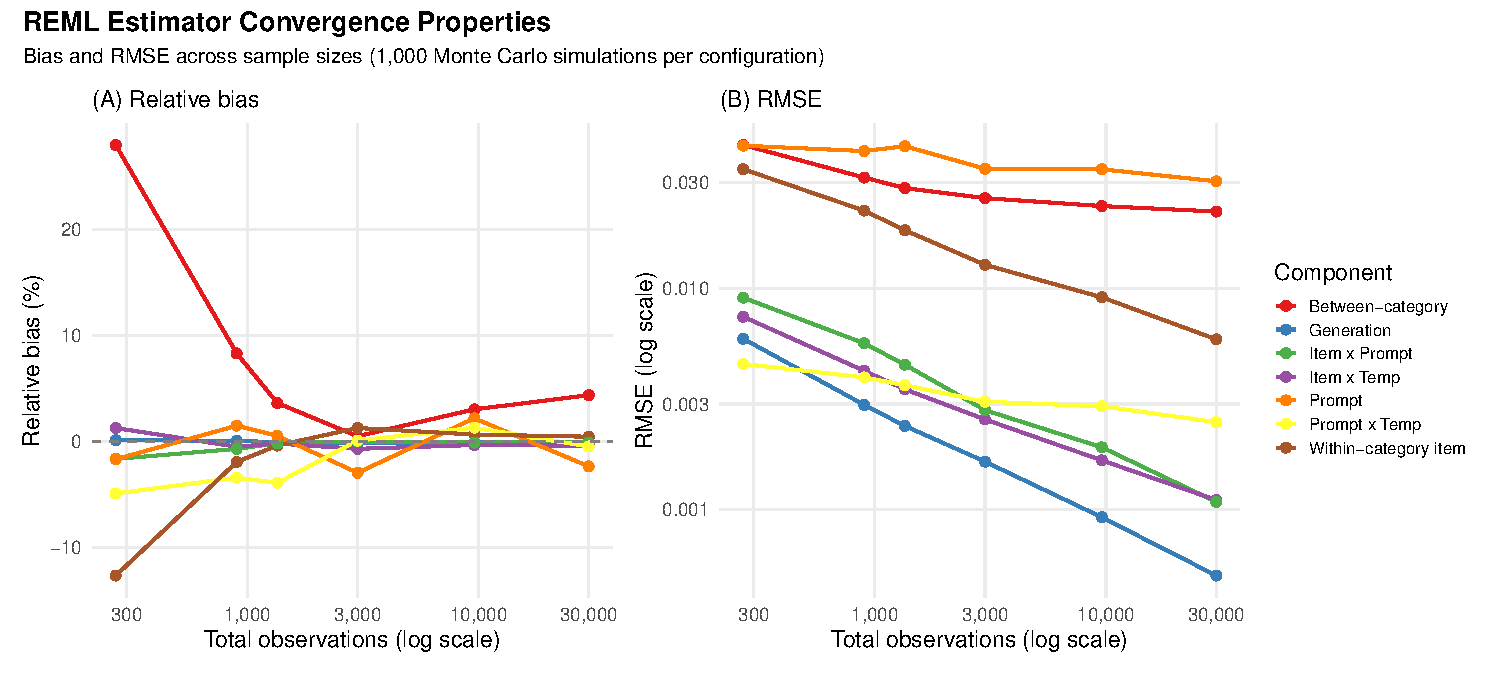
\includegraphics[width=\textwidth]{manuscript_fig1_convergence.pdf}
\caption{REML estimator convergence. (a)~Bias falls below 5\% for all components once total observations exceed 1,000. (b)~RMSE by component across sample sizes, showing monotonic decline. Interaction components ($\sigma^2_{\alpha\phi}$, $\sigma^2_{\alpha\lambda}$) require larger samples for precise estimation than main effects. 1,000 simulations per configuration.}
\label{fig:convergence}
\end{figure}

\subsection{Robustness Studies}\label{si:robustness}

Four studies probe how the variance decomposition and D-study projections degrade under specific assumption violations, and the framework holds up across all four.

\phantomsection\label{si:additivity}
Three-way item$\times$variant$\times$temperature interactions barely move the decomposition. Sweeping their magnitude from 0 to 100\% of the largest two-way component ($N = 50$, $C = 5$, $V = 4$, $H = 3$, $R = 5$) shifts Kendall's $\tau$ on the D-study ranking only from 0.895 to 0.877 at maximum violation, and non-residual components show under 5\% relative bias across all levels.

Per-stratum REML recovers heteroscedastic residuals to within 0.3\% relative bias. With temperature-specific residuals at $\sigma^2_{\epsilon,0} = 0.005$, $\sigma^2_{\epsilon,0.7} = 0.04$, and $\sigma^2_{\epsilon,1.0} = 0.08$, fitting a separate mixed-effects model per temperature via \texttt{lme4::lmer} recovers each within 0.3\% bias. A single homoscedastic \texttt{lmer} fit pools to a weighted average instead, and the \texttt{glmmTMB} dispersion model substantially overestimates residual variance. Non-residual components remain unbiased under all three estimators.

\phantomsection\label{si:small_v}
$\hat{\sigma}^2_\phi$ is imprecise at small $V$, so we recommend $V \geq 3$. We swept $V \in \{2, 3, 4, 5, 7, 10\}$ and $\sigma^2_\phi \in \{0, 0.04, 0.10\}$. At $\sigma^2_\phi = 0.10$, RMSE falls from 0.156 at $V = 2$ to 0.105 at $V = 3$ and 0.049 at $V = 10$. For both nonzero values of $\sigma^2_\phi$, relative bias is 3.8 - 5.3\% at $V = 2$ and 1.0 - 4.5\% at $V \geq 3$ (Figure~\ref{fig:small_k}). Each of these bias estimates is within two Monte Carlo SEs of zero, so the simulation does not show that bias falls as $V$ grows. A knife-edge test shows directional accuracy collapses to near chance when prompts and replications contribute equally, but recovers when one source clearly dominates.

\begin{figure}[h]
\centering
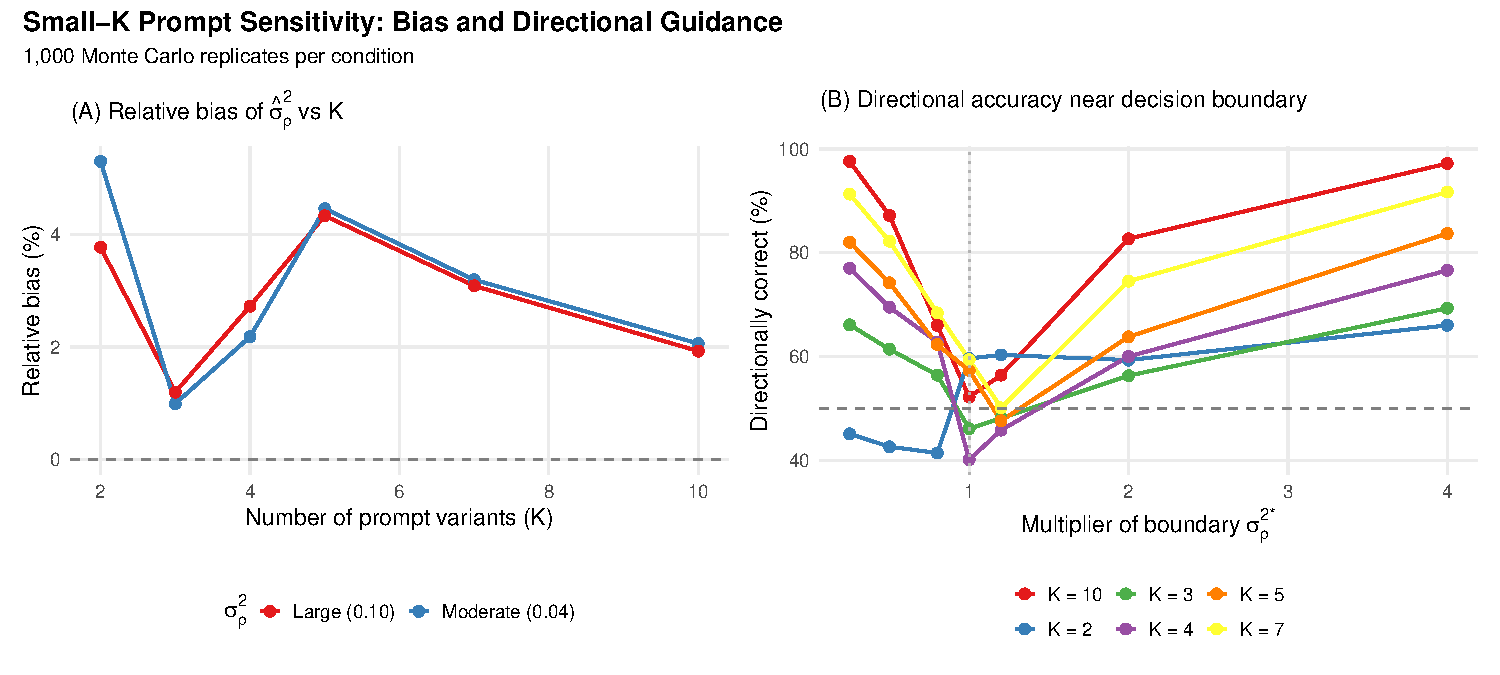
\includegraphics[width=\textwidth]{manuscript_fig2_small_k.pdf}
\caption{Small-$V$ prompt sensitivity estimation. (a)~Relative bias of $\hat{\sigma}^2_\phi$ versus number of prompt variants $V$. Bias is 3.8 - 5.3\% at $V\!=\!2$ and 1.0 - 4.5\% at $V \geq 3$, within two Monte Carlo SEs of zero throughout. The recommendation of $V \geq 3$ rests on RMSE (see text). (b)~Directional accuracy of the D-study recommendation (add prompts vs.\ add replications) near the knife-edge boundary where both interventions yield equal gains. Accuracy drops to near chance at the boundary. Away from it, accuracy rises with $V$: within this sweep it peaks at 66\% at $V\!=\!2$ and exceeds 90\% only at $V \geq 7$. 1,000 replicates per condition. Axis label uses $K$ for prompt variants (simulation convention). $K = V$ in main text notation.}
\label{fig:small_k}
\end{figure}

D-study projections transfer imperfectly between model profiles but identify the right top intervention most of the time. Across two profiles (a low-noise frontier model and a high-noise cheaper model), component estimates carry 55 - 59\% relative error when frontier components project to the cheaper profile, and 127 - 154\% in the reverse direction, but the projected top intervention is nonetheless incorrect only 9 - 13\% of the time.

\subsection{D-Study Projection Validation Under Misspecification}
\label{si:dstudy_validation}

We stress-test D-study projections under five scenarios. Scenario 1 is a correctly specified baseline. The other four perturb the DGP along a different axis each: correlated random effects ($\alpha = 2$), non-exchangeable prompt clusters (ratio of 8 between cluster variances), heavy-tailed score residuals (Student-$t$ with df $= 5$), and heterogeneous category $\times$ variant variance (a $0.25\times$ vs.\ $4\times$ ratio across categories). Each scenario draws 1{,}000 Monte Carlo replicates from its DGP. We fit the standard TEE model and compare projected variance components against the truth. The relative bias in the projected variance ranges from $-7.2\%$ (heavy-tailed) to $-0.9\%$ (baseline), with the other three between $-2.3\%$ and $-1.6\%$ (Table~\ref{tab:dstudy_misspec}). All five scenarios produce $|\text{bias}| \leq 8\%$, supporting the framework under the assumption violations tested.

\begin{table}[h]
\centering
\small
\caption{D-study projection bias under five scenarios: one correctly specified baseline and four misspecification conditions (correlated random effects, non-exchangeable prompts, heavy-tailed scores, heterogeneous category interactions). All scenarios produce $|\text{bias}| \leq 8\%$, confirming that D-study projections are stable under the assumption violations tested. $N_\text{sim} = 1,000$.}
\label{tab:dstudy_misspec}
\begin{tabular}{llr}
\toprule
Scenario & Key parameter & Rel.\ bias (\%) \\
\midrule
1. Correct specification & - & $-0.9$ \\
2. Correlated RE & $\alpha = 2$ & $-2.0$ \\
3. Non-exchangeable prompts & ratio $= 8$ & $-1.6$ \\
4. Non-normal scores & df $= 5$ & $-7.2$ \\
5. Heterogeneous category $\times$ variant & 0.25/4$\times$ & $-2.3$ \\
\bottomrule
\end{tabular}
\end{table}

\begin{figure}[h]
\centering
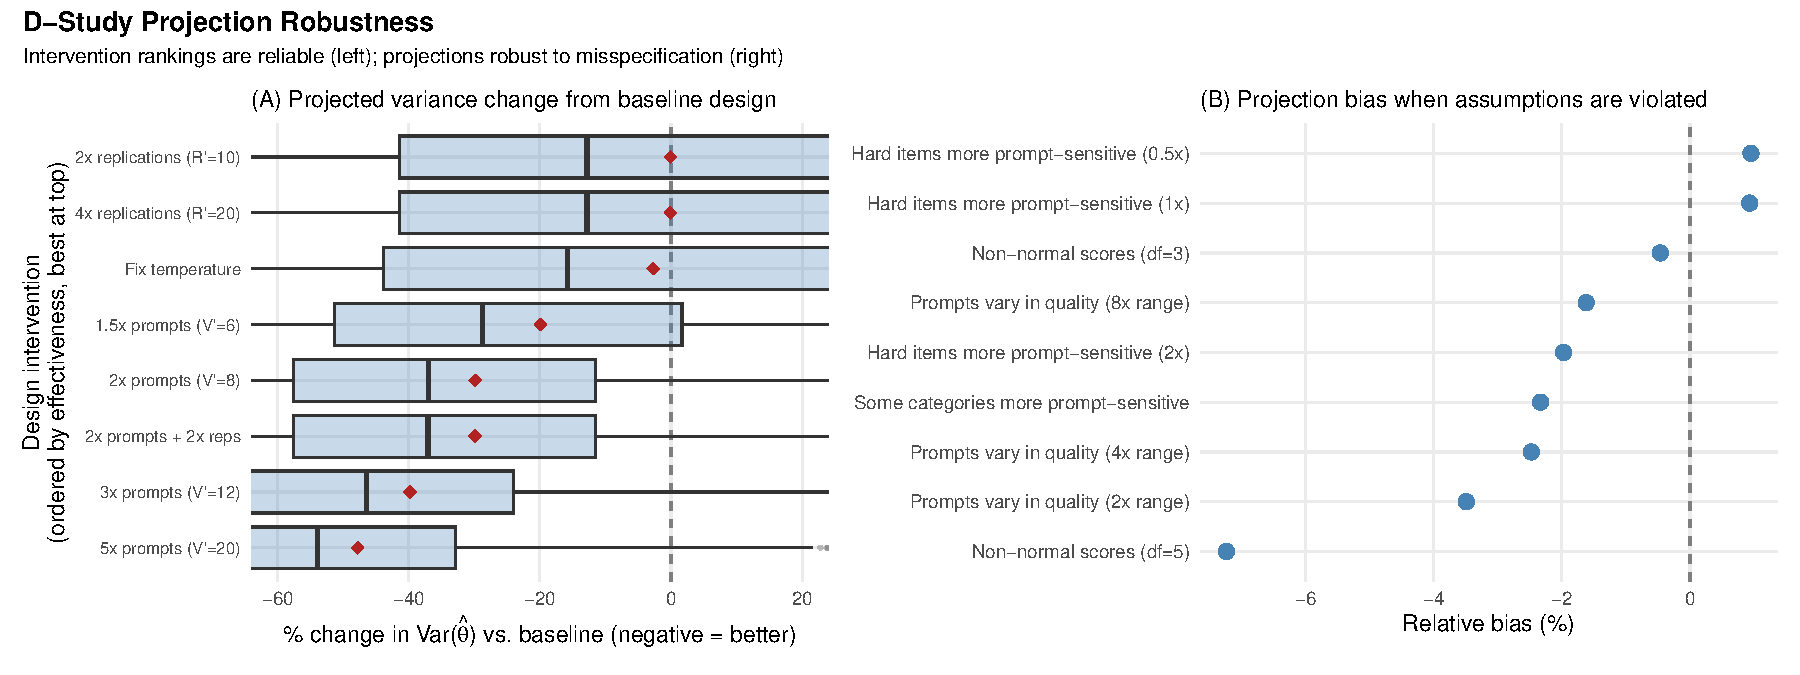
\includegraphics[width=\textwidth]{manuscript_fig3_dstudy.pdf}
\caption{D-study projection validation. (a)~Projected \% change in variance for each intervention (1,000 datasets). Red diamonds: true change. (b)~Projection accuracy under assumption violations, with bias $\leq 8\%$. Details in Section~\ref{si:dstudy_validation}.}
\label{fig:dstudy_robustness}
\end{figure}

\subsection{Scoring Method Recovery Under Judge Heterogeneity}
\label{si:scoring_recovery}

The choice of scoring method is another important design decision in LLM evaluation. Because the TEE decomposition takes observed scores as given and partitions their variance, it does not directly diagnose problems in the scoring function itself; if a scoring format introduces systematic distortions, a D-study based on those scores can point toward the wrong design changes.

In practice, three well-known LLM judge behaviors tend to degrade absolute rating scales more than pairwise comparisons, largely for the same structural reason:
\begin{enumerate}
\item \emph{Central tendency compression}, where judges cluster ratings near the middle of the scale \citep{esmaeili2025quantitative} and lose resolution at the tails. In a pairwise comparison, both items appear in the same context window, so compression affects both responses similarly and preserves their relative order.
\item \emph{Low self-consistency}, where repeated calls assign different ratings to the same item (with intra-rater agreement as low as $\alpha \approx 0.27$, \citealt{haldar2025roulette}). In pairwise comparisons, call-level anchoring noise applies to both responses simultaneously and cancels out in the difference.
\item \emph{Scale-use heterogeneity} (analogous to differential item functioning across raters, \citealt{holland1993differential}), where different judges map perceived quality onto numerical scales differently. Pairwise comparisons are unaffected by linear or multiplicative differences in scale use because the rescaling preserves the sign of the difference between two items, even though nonlinear distortions can still matter.
\end{enumerate}

Because calibrating a common numerical scale across diverse LLM judges is difficult, fitting pairwise preferences with a Bradley-Terry (BT) model avoids the scale-calibration problem—which is why benchmarks like Chatbot Arena \citep{chiang2024chatbot} rely on pairwise comparisons. That said, whereas Likert scales can suffer from reduced discriminability similar to survey satisficing \citep{krosnick1991response}, pairwise comparisons require more API calls per item set and introduce position bias.

To compare these formats under controlled conditions, we run a simulation that generates items with known latent quality scores, applies Likert and Bradley-Terry (BT) scoring under identical per-observation noise \citep{peysakhovich2015pairwise}, and varies five Likert distortions: central tendency compression ($\kappa$), per-observation anchoring noise ($\sigma_\text{anchor}$), scale-use heterogeneity ($\sigma_\text{slope}$), nonlinear scale distortion ($\gamma$), and discretization loss (number of scale points). Giving both scoring methods the same per-observation noise isolates the structural effect of the comparison format from differences in noise levels. We run four simulation experiments across these parameters: (1) ideal conditions, (2) a 3-way sweep of $\kappa \times \sigma_\text{anchor} \times \sigma_\text{slope}$ (64 conditions), (3) $\kappa \times \gamma \times$ scale points (48 conditions), and (4) a full 5-way grid (768 conditions).

As expected, under ideal conditions Likert matches full-budget BT ($\tau \approx 0.835$), but when any of the five scale distortions are present, Likert ranking recovery drops while BT remains stable (Figure~\ref{fig:scoring_recovery}). Central tendency compression has the largest impact: as $\kappa$ decreases from 1.0 to 0.3, Likert $\tau$ falls from 0.46 to 0.43 while BT stays flat at 0.50, and coarsening the scale to 3 points further reduces Likert recovery to $\tau = 0.38$. The difference is largest at low prevalence, where binary classification drops from $\tau = 0.60$ at 50\% prevalence to $\tau = 0.06$ at 0.05\% prevalence while BT remains at $\tau \approx 0.73$. This low-prevalence regime is particularly relevant for safety benchmarks like AILuminate, where a 94\% safe rate leaves relatively few unsafe cases.

These results suggest three practical guidelines: when judges are well calibrated and use finer scales (7+ points, $\kappa > 0.7$), Likert and pairwise scoring recover rankings similarly and Likert requires roughly one-third as many calls; when judge calibration is uncertain or the scale is coarse (3 - 5 points), pairwise comparisons offer much greater stability against compression, anchoring, and scale-use differences at roughly $3\times$ the cost; and for binary outcomes with low base rates ($<5\%$), pairwise comparisons perform substantially better than binary classification. Of course, realizing the benefits of pairwise scoring requires controlling for position bias: in an earlier naive-prompt run we observed a 67\% B-rate across the three judges, so our reference pipeline uses a CoT prompt, order counterbalancing, and a position covariate to keep residual position bias in check (SI Appendix, Section~\ref{si:pilot}).

\begin{figure}[h]
\centering
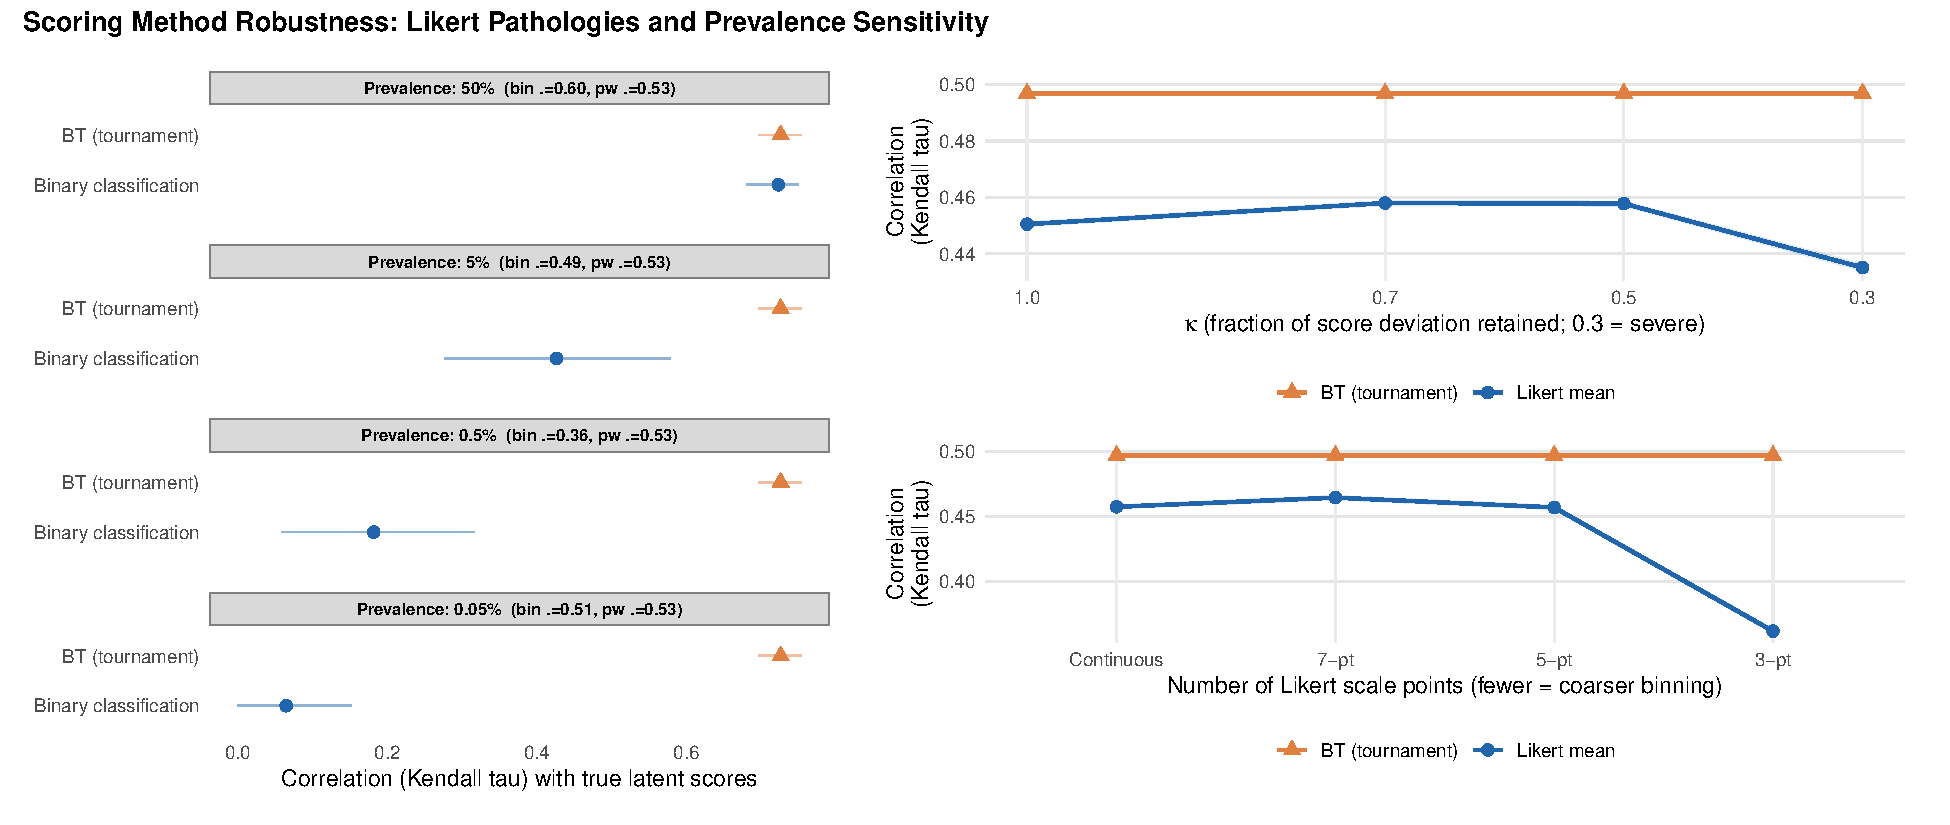
\includegraphics[width=\textwidth]{manuscript_fig_scoring_compound.pdf}
\caption{BT pairwise scoring is stable under Likert pathologies. Left: at low prevalence, binary classification collapses while BT remains stable. Upper right: central tendency compression ($\kappa$) degrades Likert ranking recovery, while BT is unaffected. Lower right: coarser Likert scales (fewer points) reduce recovery, while BT is invariant to discretization. The full simulation sweeps five pathologies ($\kappa$, $\sigma_\text{anchor}$, $\sigma_\text{slope}$, nonlinear $\gamma$, discretization). This figure shows the three with the largest effects. $N_\text{sim} = 200$.}
\label{fig:scoring_recovery}
\end{figure}

\subsection{Variance Underestimation When Pipeline Factors Are Omitted}\label{si:underestimation_sim}

The main text (Figure~\ref{fig:underestimation}) shows that naive CIs fail when the fitted model omits random effects for pipeline factors that contribute variance. This section details the six scenarios behind that result and traces how coverage degrades as design-side components are omitted from the fitted model.

We set the pipeline components to comparable magnitudes in the DGP so that each scenario captures a visible share of the variance (Table~\ref{tab:underestimation_dgp}). This setup illustrates the mechanism and is not calibrated to any benchmark. The full factorial uses $V = 4$ prompt variants, $H = 3$ temperatures, $M = 3$ judges, and $R = 8$ replications.

\begin{table}[h]
\centering
\small
\caption{DGP parameters for the variance underestimation simulation (\texttt{analysis/04g2\_sim\_underestimation\_balanced.R}). Temperature and judge enter as fixed levels; every other component is a random-effect variance.}
\label{tab:underestimation_dgp}
\begin{tabular}{lll}
\toprule
\textbf{Component} & \textbf{Value} & \textbf{Notes} \\
\midrule
$\sigma^2_\alpha$ (item)            & 0.10 & \\
$\sigma^2_\phi$ (prompt)            & 0.04 & \\
$\tau$ (temperature levels)         & $\{-0.20, 0, 0.20\}$ & $\mathrm{pop\_var}(\tau) = 0.027$ \\
$\lambda$ (judge levels)            & $\{-0.20, 0, 0.20\}$ & $\mathrm{pop\_var}(\lambda) = 0.027$ \\
$\sigma^2_{\alpha\phi}$ (item $\times$ prompt) & 0.04 & \\
$\sigma^2_{\alpha\tau}$ (item $\times$ temperature) & 0.03 & \\
$\sigma^2_{\alpha\lambda}$ (item $\times$ judge) & 0.04 & \\
$\sigma^2_{\phi\tau}$, $\sigma^2_{\phi\lambda}$, $\sigma^2_{\tau\lambda}$ & 0.02 & design $\times$ design \\
$\sigma^2_\epsilon$ (cell-level)    & 0.04 & constant across replicates within a cell \\
$\sigma^2_\rho$ (replicate)         & 0.10 & within-cell replicate noise \\
\bottomrule
\end{tabular}
\end{table}

Six scenarios sample from this factorial and fit progressively richer \texttt{lmer} models (Table~\ref{tab:underestimation_scenarios}). Scenario A is the naive baseline. It samples one observation per item at a randomly chosen (prompt, temperature, judge) configuration and reports $\mathrm{SE} = s/\sqrt{N}$. Scenarios B, C, and D then add prompt-variant, judge, and temperature random effects in turn, sampling the corresponding factor in full. Scenario E adds the design-by-design interactions. Scenario F fits cell means with the item interactions as well, which separates the cell-level term $\sigma^2_\epsilon$ from replicate noise.

\begin{table}[h]
\centering
\small
\caption{Scenarios A - F progressively enrich the fitted random-effects model. Each row indicates the factorial dimensions the scenario samples, the random effects it adds, the variance it then captures, and what remains uncaptured.}
\label{tab:underestimation_scenarios}
\resizebox{\linewidth}{!}{%
\begin{tabular}{lllll}
\toprule
\textbf{Scenario} & \textbf{Sampled} & \textbf{Adds} & \textbf{Captures} & \textbf{Misses} \\
\midrule
A (naive) & $V{=}1, M{=}1, H{=}1, R{=}1$ & $s/\sqrt{N}$ & - & all design-side \\
B         & $V{=}4, M{=}1, H{=}1, R{=}8$ & \texttt{(1|variant)}        & $\sigma^2_\phi$    & $\tau, \lambda$, interactions \\
C         & $V{=}4, M{=}3, H{=}1, R{=}8$ & + \texttt{(1|judge)}        & + $\lambda$ & $\tau$, interactions \\
D         & $V{=}4, M{=}3, H{=}3, R{=}8$ & + \texttt{(1|temp)}         & + $\tau$  & interactions \\
E         & same data as D               & + \texttt{(1|variant:judge), (1|variant:temp), (1|temp:judge)} & + design $\times$ design & item $\times$ design, $\sigma^2_\epsilon$ \\
F         & cell means of D's data       & + \texttt{(1|item:variant), (1|item:judge), (1|item:temp)} & + item $\times$ design, $\sigma^2_\epsilon$ & - \\
\bottomrule
\end{tabular}}
\end{table}

The point estimate in every scenario is the mean of the sampled observations. The SE is $\sqrt{\text{Var}(\hat\beta_0)}$ from the fitted \texttt{lmer}, except for A, which uses $s/\sqrt{N}$. A fit that exceeds a 300-second timeout falls back to the oracle SE computed from the true variance components under that scenario's model; this happened in 28 of the 1,000 Scenario E replicates at $N = 400$ and in no other cell. All six scenarios are evaluated at $N \in \{25, 50, 100, 200, 400\}$ with 1,000 Monte Carlo replicates per cell.

Coverage rises in steps across the six scenarios as each fit captures more of the design-side variance. Scenario A captures none of it. Its SE is the naive $s/\sqrt{N}$ and shrinks with sample size, but the bias from the single (prompt, temperature, judge) configuration stays constant, so coverage falls from 42\% at $N = 25$ to 11\% at $N = 400$. Scenario B adds prompt-variant random effects and reaches 56 - 64\% coverage, which stays well below nominal because the judge and temperature offsets are still unmodeled. Scenario C adds judges and reaches 86 - 89\%, limited by the remaining temperature offset. Scenarios D, E, and F capture every design-side component and cover at 99 - 100\%, above nominal, with SEs 9 - 19\% larger than the oracle SE. Because the DGP holds the three judges and three temperature levels fixed, they add no error to the estimate. Both the fitted and the oracle SE still count the judge and temperature variance, since those SEs generalize to new judges and temperatures. The fitted SEs are therefore 1.5 - 1.7 times the empirical standard deviation of the estimates. Section~\ref{si:underestimation_redraw} redraws the levels in every replicate. E and F have identical coverage at this design, but F also separates the cell-level term $\sigma^2_\epsilon$ from replicate noise, which matters when $\sigma^2_\epsilon$ is large.

\begin{figure}[h]
\centering
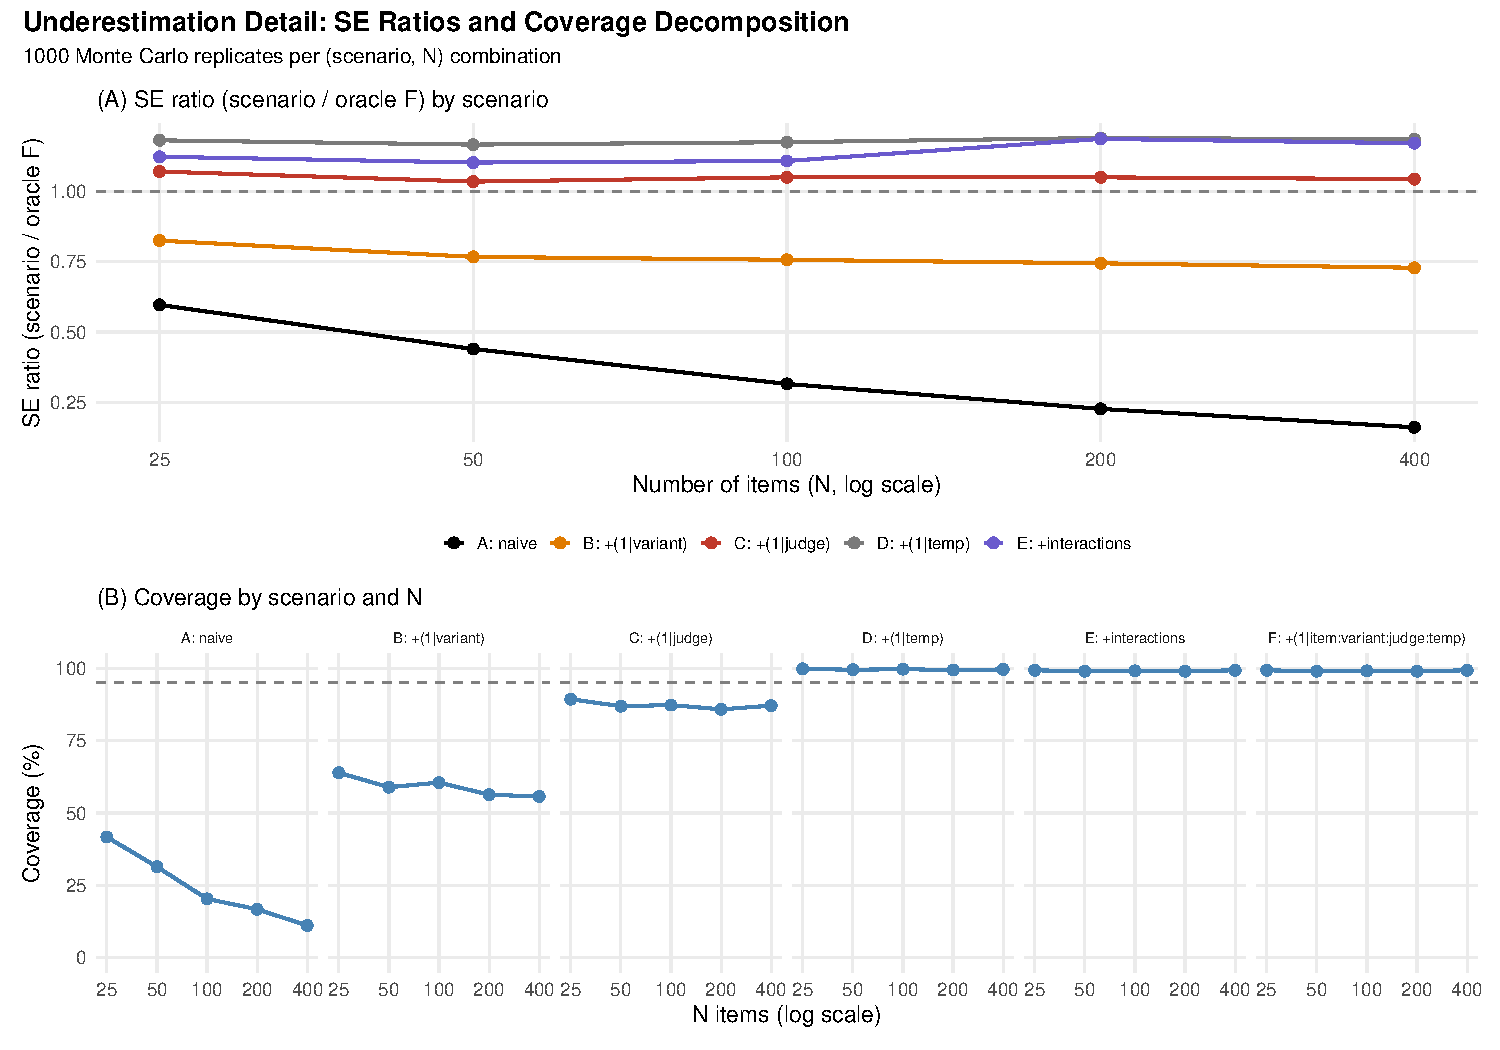
\includegraphics[width=\textwidth]{manuscript_fig_underestimation_detail_v2.pdf}
\caption{Naive 95\% CIs lose coverage as sample size grows because the SE shrinks while the bias from omitted pipeline factors stays constant. Panel (a) plots each scenario's SE relative to the oracle SE of the full model, with the naive Scenario A about $6\times$ smaller at $N = 400$. Panel (b) plots 95\% CI coverage versus $N$ for the six scenarios, showing how each added random effect (prompt in B, judge in C, temperature in D, interactions in E and F) closes one more component of the omitted variance and lifts coverage toward nominal. $N \in \{25, 50, 100, 200, 400\}$; $N_\text{sim} = 1,000$.}
\label{fig:underestimation_detail}
\end{figure}

\subsection{Coverage When Judge and Temperature Levels Are Redrawn}\label{si:underestimation_redraw}

Section~\ref{si:underestimation_sim} holds the three judge levels and the three temperature levels fixed at $\{-0.20, 0, 0.20\}$, so Scenarios D - F over-cover. Here each replicate draws new judge and temperature levels from $N(0, 0.027)$, the variance of the fixed levels, and the estimand is the superpopulation mean $\mu$. The DGP, scenarios, fitted models, seeds, and 1,000 replicates per cell are unchanged (\texttt{analysis/04g2\_sim\_underestimation\_balanced.R --redraw-design}; comparison in \texttt{analysis/04g2b\_redraw\_comparison.R}).

Table~\ref{tab:underestimation_redraw} compares coverage under the two designs. With redrawn levels, Scenarios D, E, and F cover at 91 - 95\%. Their median SE is 0.94 - 1.07 times the empirical standard deviation of the estimates, against 1.53 - 1.69 with fixed levels. Coverage stays a few points below nominal because the judge and temperature variances each rest on three levels, so the SE itself varies from replicate to replicate. Misses concentrate where the estimated SE is small. Pooled over $N$, coverage is 80 - 85\% in the quarter of replicates with the smallest SEs and 99\% in the quarter with the largest. Scenarios A - C stay well below nominal under both designs. Six Scenario E fits at $N = 400$ timed out and used the oracle SE. We report the median SE because one Scenario E fit at each of $N = 200$ and $N = 400$ returned a degenerate SE above 1 under each design.

\begin{table}[h]
\centering
\small
\caption{Redrawing the judge and temperature levels in every replicate lowers Scenario D - F coverage from 99 - 100\% to 91 - 95\%. Cells give 95\% CI coverage (\%) by scenario, level design, and number of items $N$, with 1,000 replicates per cell (Monte Carlo SE at most 1.6 points).}
\label{tab:underestimation_redraw}
\begin{tabular}{llrrrrr}
\toprule
 & & \multicolumn{5}{c}{$N$} \\
\cmidrule(lr){3-7}
\textbf{Scenario} & \textbf{Levels} & 25 & 50 & 100 & 200 & 400 \\
\midrule
A & Fixed & 41.7 & 31.4 & 20.3 & 16.7 & 11.1 \\
A & Redrawn & 43.2 & 31.8 & 20.2 & 14.4 & 11.6 \\
\addlinespace
B & Fixed & 63.9 & 58.9 & 60.5 & 56.3 & 55.7 \\
B & Redrawn & 66.1 & 59.8 & 57.0 & 57.2 & 57.8 \\
\addlinespace
C & Fixed & 89.3 & 86.9 & 87.3 & 85.8 & 87.1 \\
C & Redrawn & 84.3 & 81.8 & 80.9 & 81.8 & 79.4 \\
\addlinespace
D & Fixed & 99.8 & 99.5 & 99.7 & 99.4 & 99.6 \\
D & Redrawn & 94.9 & 94.1 & 92.6 & 93.6 & 92.9 \\
\addlinespace
E & Fixed & 99.3 & 99.0 & 99.1 & 99.0 & 99.3 \\
E & Redrawn & 93.9 & 91.3 & 90.7 & 91.8 & 90.8 \\
\addlinespace
F & Fixed & 99.3 & 99.0 & 99.1 & 99.0 & 99.3 \\
F & Redrawn & 93.6 & 91.1 & 90.6 & 91.6 & 90.9 \\
\bottomrule
\end{tabular}
\end{table}


\subsection{Latent Item Ambiguity}\label{si:latent_ambiguity}

This simulation builds an even harsher misspecification: per-item variance heterogeneity driven by a latent ambiguity score, combined with a sparse 3-way interaction concentrated in the ambiguous tail. The motivating concern is that earlier robustness simulations addressed additivity violations (Section~\ref{si:additivity}) and correlated random effects (Section~\ref{si:dstudy_validation}) in isolation. When both arise jointly from the same latent property of the item, do D-study projections still reflect the truth?

The DGP draws a per-item ambiguity score $z_i \sim N(0, 1)$ and scales that item's item$\times$prompt and item$\times$judge variances by $1 + \gamma z_i^2$. Higher-$z_i$ items therefore swing more under prompt and judge variation. Items with $z_i > 1$ (roughly 16\% of the population) additionally carry a 3-way item$\times$prompt$\times$judge interaction with variance $0.01$, so prompt and judge effects compound nonadditively for the most ambiguous items. We sweep $\gamma$ over $\{0, 0.5, 1, 2\}$. The endpoints anchor the experiment: $\gamma = 0$ is correct specification, $\gamma = 2$ triples interaction variance one SD above the mean.

We sample a small factorial of $N = 30$ items across $C = 5$ categories, $V = 3$ prompts, $H = 2$ temperatures, $M = 3$ judges, and $R = 3$ replications, totaling 1,620 observations per fit. The TEE specification carries the two-way interactions only; the 3-way interaction and the latent heterogeneity remain outside the model.

CI coverage holds at 89 - 91\% across all four $\gamma$ settings, against the 95\% nominal under such a small $N$. The worst component-level relative bias is below 9\% and D-study intervention rankings agree perfectly with the truth (Spearman $\rho = 1.0$) across 1{,}000 simulations per setting. Breakdown by $\gamma$ in Table~\ref{tab:latent_ambiguity}.

\begin{table}[h]
\centering
\small
\caption{TEE stability under latent item ambiguity. $\gamma$ controls the strength of ambiguity-driven dependence between item difficulty and interaction variances, with sparse 3-way interactions for ambiguous items ($z_i > 1$). CI coverage does not degrade, component bias stays below 9\%, and D-study intervention rankings are preserved exactly across all ambiguity levels. $N_\text{sim} = 1,000$.}
\label{tab:latent_ambiguity}
\begin{tabular}{llrrr}
\toprule
$\gamma$ & Label & Coverage (\%) & Max $|\text{rel.\ bias}|$ (\%) & D-study $\rho$ \\
\midrule
0   & Baseline    & 90.5 & 8.8 & 1.00 \\
0.5 & Mild        & 88.7 & 6.7 & 1.00 \\
1   & Moderate    & 90.3 & 3.4 & 1.00 \\
2   & Strong      & 91.2 & 6.0 & 1.00 \\
\bottomrule
\end{tabular}
\end{table}

This stability follows from the fact that \texttt{lmer} estimates \emph{marginal} variance components (i.e., population averages across items rather than item-specific variances). When each item's item$\times$prompt component is scaled by $1 + \gamma z_i^2$, the expected scaling across the population is $E[1 + \gamma z_i^2] = 1 + \gamma$, yielding a marginal item$\times$prompt variance of $(1 + \gamma)\sigma^2_{\alpha\phi}$, which the estimator recovers. Meanwhile, because the sparse 3-way interaction is limited to a small subset of items, it is absorbed into the residual term and only slightly increases $\hat{\sigma}^2_\epsilon$, leaving the two-way estimates largely unaffected.

Untested scenarios include multimodal residuals (e.g., from a mixture of refusals and compliance), extreme base rates (above 0.9 or below 0.1), unbalanced designs with missing cells, post-hoc model specification search, and nonlinear temperature effects.


%% ============================================================================
%% SI SECTION 4: MULTI-TURN AND MULTI-AGENT EXTENSIONS
%% ============================================================================

\clearpage

\section{Multi-Turn and Multi-Agent Extensions}
\label{si:extensions}

\subsection{Multi-Turn Extension}

The single-turn DGP extends to multi-turn evaluation when each turn's score depends on the prior conversation. Adding a turn index $t$ and a turn-conditional mean $\mu_t(\mathbf{h}_{<t})$ for the expected score given history $\mathbf{h}_{<t}$ yields\footnote{In this subsection $\eta(t)$ denotes the hazard rate and $\mathbf{h}_{<t}$ denotes conversation history, distinct from the subscript $h$ used for temperature in the main DGP.}
\begin{equation}
Y_{t,ivhm}^{(r)} = \mu_t(\mathbf{h}_{<t}) + \alpha_i + \phi_v + \tau_h + (\alpha\phi)_{iv} + \epsilon_{t,ivhm} + \rho_{t,ivhm}^{(r)}.
\end{equation}
The pipeline-side variance components keep their single-turn interpretations because they describe how the evaluation is computed, not how the conversation evolves. The multi-turn structure enters through $\mu_t(\mathbf{h}_{<t})$, which drifts as the model conditions on accumulating context.

Safety evaluation often asks at what turn the model first crosses a safety threshold $\theta^*$, which maps onto a survival framing with hazard rate
\begin{equation}
\eta(t) \approx \Phi\!\left(\frac{\mu_t(\mathbf{h}_{<t}) - \theta^*}{\sqrt{\text{TEE}_t}}\right).
\end{equation}
This Gaussian-tail approximation treats $\eta(t)$ as the probability that a Gaussian score with mean $\mu_t(\mathbf{h}_{<t})$ and variance $\text{TEE}_t$ exceeds the threshold $\theta^*$. Larger pipeline-level variance therefore means a higher hazard at any threshold above $\mu_t(\mathbf{h}_{<t})$, so the same components that distort single-turn CIs also raise multi-turn safety risk. Full integration with Cox proportional hazards models \citep{cox1972regression} for time-varying covariates is beyond the current scope. Existing empirical work supports the framing. \citet{weng2025footinthedoor} document harmfulness scores increasing across turns under foot-in-the-door attacks, consistent with $\mu_t(\mathbf{h}_{<t})$ drifting upward as context accumulates. \citet{li2025timetoincon} fit hazard models to multi-turn LLM interactions and find that hazard rates depend on temperature, supporting the inclusion of $\tau_h$ in the multi-turn DGP.

\subsection{Multi-Agent Extension}

Suppose instead that a pipeline runs $A$ agents in parallel on the same item, yielding $Y_1,\ldots,Y_A$, and reports their average $\bar Y$. The variance of the mean is
\begin{equation}
\Var(\bar{Y}) = \frac{1}{A^2}\left[\sum_{a=1}^{A} \text{TEE}_a + \sum_{a \neq a'} \Cov(Y_a, Y_{a'})\right].
\end{equation}
Averaging reduces each agent's TEE component at a rate of $1/A$. However, the off-diagonal covariance terms do not disappear when agents share training data or scoring rubrics, and correlated errors across agents reduce the gains from ensembling. A multi-judge panel scoring a single response is a special case of this setup, with judges as the parallel agents.

When agents are chained sequentially so that agent $A$ takes its input from agent $A-1$, the variance of the final score decomposes via the law of total variance:
\begin{equation}
\Var(Y_A) = \E[\Var(Y_A \mid Y_{A-1})] + \Var(\E[Y_A \mid Y_{A-1}]).
\end{equation}
Here, the first term reflects the variance introduced by agent $A$ conditional on its input, while the second term captures the variance propagated from upstream steps. Applying this recursion across the chain splits overall variance into each agent's local contribution and the variance that it inherits from upstream \citep{duan2025uprop}. Consistent with this structure, \citet{kim2025scaling} find $17.2\times$ error amplification for independent agent topologies compared with $4.4\times$ for centralized ones, suggesting that agent architecture can affect pipeline variance as much as judge or prompt selection.



\clearpage

\section{GLMM Robustness Check}
\label{si:glmm}

Binary outcomes in the main text use a linear probability model \citep[LPM,][]{angristpischke2009}. The LPM residuals for binary data are heteroscedastic, which raises the question of whether the variance shares that we report in the main text are artifacts of the link function. To check, we refit the three binary decompositions with a logit link via \texttt{lme4::glmer(family = binomial)} \citep{bates2015lme4} and compare the GLMM shares with the LPM shares used in the main text.

\begin{table}[ht]
\centering
\caption{LPM vs.\ GLMM Var($\hat\theta$) decomposition for the three binary benchmarks (pairwise ideology, safety classification, MMLU). LPM shares are on the probability scale; GLMM shares are on the logit scale, so absolute SE values are not directly comparable, but component rankings are. For the GLMM, the level-1 residual is fixed at $\pi^2/3$ following the logistic-link convention \citep{nakagawa2010repeatability}. All three fits include the cell-level random effect. For MMLU the model layer is the system under test (SUT) rather than a judge. The SUT row plays the same role as ``judge model'' in the other two benchmarks. Spearman rank correlations between LPM and GLMM shares are $\rho = 0.99$ (pairwise), $0.91$ (safety), and $0.95$ (MMLU), confirming that the dominant components are not LPM artifacts.}
\label{tab:glmm_comparison}
\footnotesize
\begin{tabular}{lrrrrrr}
\toprule
& \multicolumn{2}{c}{\textbf{Pairwise (\%)}} & \multicolumn{2}{c}{\textbf{Safety (\%)}} & \multicolumn{2}{c}{\textbf{MMLU (\%)}} \\
\cmidrule(lr){2-3} \cmidrule(lr){4-5} \cmidrule(lr){6-7}
\textbf{Component} & \textbf{LPM} & \textbf{GLMM} & \textbf{LPM} & \textbf{GLMM} & \textbf{LPM} & \textbf{GLMM} \\
\midrule
Judge / SUT model ($\sigma^2_\lambda$, sensitivity) & 68.4 & 50.9 & 43.8 & 70.7 &  6.7 &  7.6 \\
Within-category item ($\sigma^2_\delta$)            &  7.6 & 13.7 & 20.8 & 11.4 & 72.2 & 71.4 \\
Prompt ($\sigma^2_\phi$)                            &  0.4 &  0.4 &  0.0 &  0.0 &  0.4 &  1.3 \\
Item $\times$ judge / SUT ($\sigma^2_{\alpha\lambda}$) &  1.9 &  1.9 & 16.7 &  4.3 & 10.5 &  5.2 \\
Prompt $\times$ judge / SUT ($\sigma^2_{\phi\lambda}$) &  0.1 &  0.0 & 12.4 &  7.9 &  1.3 &  4.4 \\
Position ($\sigma^2_\pi$, sensitivity)              & 20.9 & 32.7 & -    & -    & -    & -    \\
Between-category ($\sigma^2_\kappa$)                &  0.2 &  0.1 &  4.9 &  4.7 &  7.7 &  9.6 \\
Other ($\leq$1\%)                                   &  0.5 &  0.3 &  1.4 &  1.0 &  1.2 &  0.6 \\
\bottomrule
\end{tabular}
\end{table}

The decomposition holds up under the logit link in all three benchmarks. The same component dominates in each case (judge model on pairwise and safety, within-category item heterogeneity on MMLU), and rank correlations are near-perfect ($\rho = 0.99$ pairwise, $0.91$ safety, $0.95$ MMLU). For safety, the judge model share rises from 43.8\% under the LPM to 70.7\% under the GLMM. This is because the safe rate is 94\%, and at that rate a small difference between judges on the probability scale becomes a large difference on the logit scale. For MMLU, where 84.5\% of answers are correct, item heterogeneity is the largest component under both links (72.2\% LPM, 71.4\% GLMM), and the three prompt terms are small on both scales (2.7\% and 6.1\%). We keep the LPM in the main text because we can read its components directly as percent of variance on the probability scale. We use the GLMM here only to check robustness to the link function.



\clearpage

\section{Ideology Scoring Comparison: Likert vs Pairwise}
\label{si:scoring_comparison}

When we apply Likert and pairwise scoring to the same domain under a matched protocol, they produce qualitatively different variance profiles, which have different implications for optimizing the pipeline.\footnote{An initial pairwise run used a naive prompt (forced A/B, no CoT) and an older judge set (GPT-4o, Gemini~2.0~Flash, Claude~Haiku~4.5). That run was dominated by recency bias (Haiku selected the second response 91\% of the time regardless of content, GPT-4o 70\%, Gemini 39\%), so the raw decomposition attributed 20.7\% of variance to a ``judge main effect'' that was really position bias. Recoding via \texttt{true\_order} reduces this spurious main effect to 0.2\%, but the noise from the position bias moves into the item$\times$judge interaction, which rises to 54.7\%. This happens because Haiku's near-random content signal becomes item-level disagreement after recoding. The naive pairwise data is archived. The reference pairwise pipeline described above uses the CoT protocol and a judge set chosen for lower recency bias. We also re-ran the Likert pipeline with the same CoT protocol and judges, so the two pipelines now differ only in the rating format. The earlier naive-Likert run is archived.} Four frontier LLMs (Claude~Opus~4.5, GPT-5.1, DeepSeek~Chat~v3.1, Grok~4.1~Fast) generated free-text responses to prompts drawn from five ideology dimensions. A common judge panel and prompt protocol then scored each response under either a 1 - 5 Likert scale or a forced pairwise A/B comparison.

Both pipelines use a chain-of-thought (CoT) prompt with a content-markers reasoning step, an explicit instruction not to let presentation order or prompt wording bias the decision, and a structured JSON output. The judges are \texttt{openai/gpt-oss-120b}, \texttt{google/gemini-2.0-flash-001}, and \texttt{deepseek/deepseek-chat-v3.1}, with each cell replicated 3 times at 3 temperatures (0, 0.7, 1.0) across 5 paraphrased prompt variants. The Likert pipeline makes 150~items $\times$ 5~variants $\times$ 3~temperatures $\times$ 3~judges $\times$ 3~replications $= 20,250$ calls. The pairwise pipeline judges the same 150 item-pairs in both orderings (listed + swapped), and recodes the raw A/B outcome to \texttt{model\_a\_wins} using the order randomized at item creation (\texttt{true\_order}) to remove any residual position bias. The pairwise design is also 20,250 calls.

\begin{figure}[htbp]
\centering
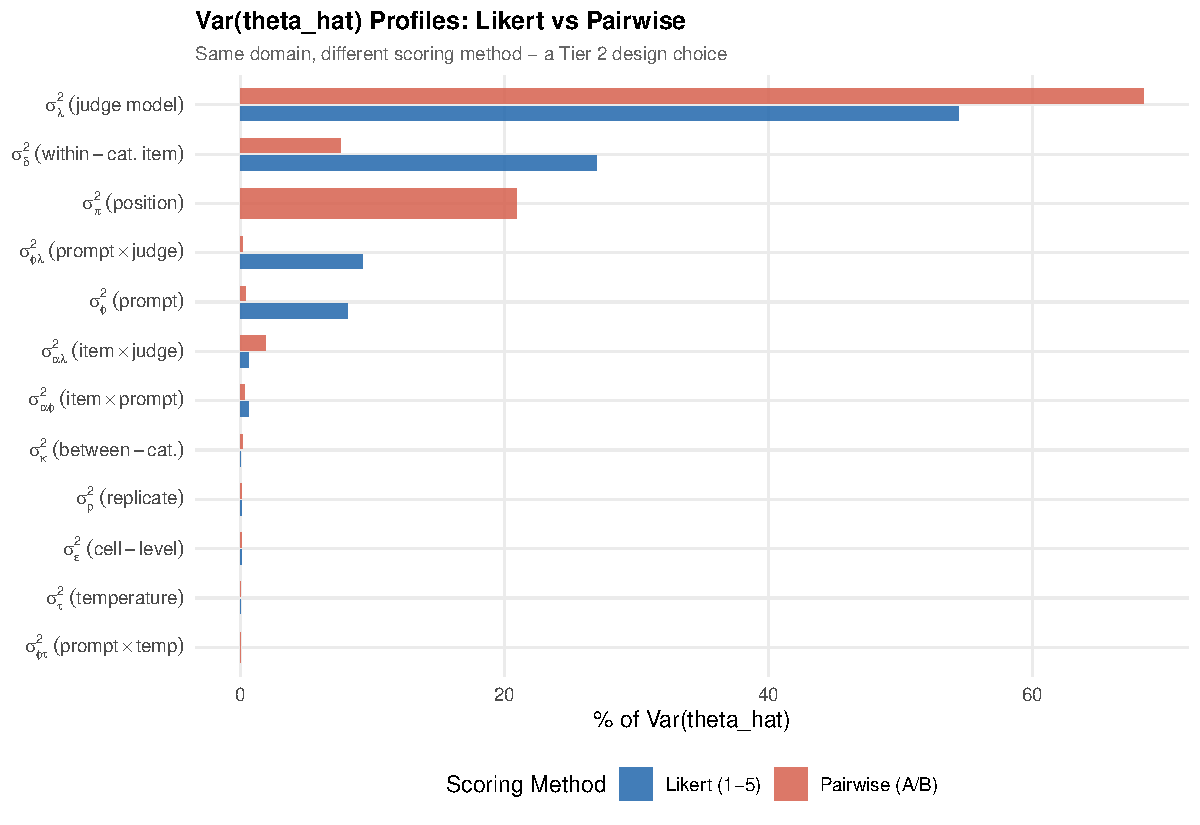
\includegraphics[width=\linewidth]{fig2_scoring_comparison.pdf}
\caption{Judge-model variance dominates both ideology pipelines, but the secondary rankings differ. After judges, Likert is dominated by item heterogeneity and pairwise by position bias, a factor with no Likert analogue. Operational design: $N{=}150$, $V{=}5$, $M{=}3$, $H{=}3$, $R{=}3$ (pairwise also crosses $P{=}2$ position orderings).}
\label{fig:variance_comparison}
\end{figure}

In both decompositions, judge-model design sensitivity accounts for the largest share of variance (54.4\% under Likert and 68.4\% under pairwise), though the remaining components differ noticeably between the two formats. Under Likert scoring, the next largest shares come from within-category item heterogeneity (26.9\%), prompt$\times$judge interaction (9.3\%), and the prompt main effect (8.1\%). Under pairwise scoring, by contrast, the position factor (recoded from listed and swapped orderings via \texttt{true\_order}) accounts for 20.9\% of the variance on its own, while within-category item heterogeneity drops to 7.6\% and item$\times$judge falls to 1.9\%. In short, the two scoring formats face different sources of error: pairwise comparisons avoid scale compression, anchoring noise, and scale-use heterogeneity \citep{esmaeili2025quantitative, haldar2025roulette, holland1993differential}, whereas Likert scoring is not affected by presentation-order bias. As shown in Section~\ref{si:scoring_recovery}, pairwise BT remains stable under those Likert scale distortions, and it does not break down at low prevalence the way binary scoring does ($\tau = 0.06$ vs.\ $\tau = 0.73$ for BT; Figure~\ref{fig:scoring_recovery}).

Despite the different variance profiles, the D-studies for both formats point to judge variance as the key lever. %Adding judges produces the largest single variance reduction in both formats because $\sigma^2_\lambda/M$ enters with divisor $M$ alone.
Adding items, prompts, or replications buys little marginal precision once their respective terms are well-averaged at $N = 150$, $V = 5$, $R = 3$. Full per-method D-study projections appear in Figures~\ref{fig:dstudy_likert} and~\ref{fig:dstudy_pairwise}.

A separate sanity check explains why pairwise replicate noise is so large. A Claude~Sonnet~4.5 judge with a CoT prompt that \emph{allowed} a TIE option was run on all 150 pairwise items in both orderings. Inter-order consistency was 100\% (every item's listed and swapped judgments either inverted cleanly or both returned TIE), confirming zero position bias. Sonnet returned TIE on 84.7\% of items, so only 23 of 150 pairs carried a clear ideological preference. On those 23 distinguishable items, directional agreement with the three CoT pairwise judges was high (DeepSeek 100\%, Gemini 91\%, GPT-OSS 87\%). The 85\% TIE rate explains why so much pairwise variance lands in $\sigma^2_\rho$ and $\sigma^2_\epsilon$. When judges must pick a side on pairs that are genuinely similar, their choices are random with respect to content, and this noise accumulates within and across cells. The Likert pipeline avoids this problem because the 1 - 5 scale allows a centrist rating for ambiguous content.



\clearpage

\section{Pilot Study Details}
\label{si:pilot}

TEE is most useful when researchers can plan a full factorial pipeline from cheap pilot data. This section shows that variance estimates from a pilot recover the qualitative D-study conclusions of a full run, so a small pilot is enough to choose a design, which the full pipeline then confirms quantitatively.

We use the Likert ideology demonstration (150 items, 5 prompt variants, 3 temperatures, 3 judges, 3 replications; 20,250 calls) as the testbed. A 30-item, 3-variant subset of the full-run data stands in for the pilot, and we compare its D-study projections to the full-run results. Because the pilot is a subsample of the same items, this test asks whether small-sample variance estimates translate into accurate D-study projections. It does not test how a pilot drawn from completely different items would generalize.

The pilot recovers the qualitative D-study conclusions. Both pilot and full run identify judge-model design sensitivity and within-category item heterogeneity as the two dominant contributors to $\Var(\hat\theta)$. The shares differ between the two designs because the divisors differ. The pilot gives 42.4\% to judge model and 48.6\% to within-category item, and the full run gives 54.4\% and 26.9\%. The larger $N$ in the full run shrinks $\sigma^2_\delta/N$ faster than $\sigma^2_\lambda/M$ at fixed $M$, which raises the judge-model share. A pilot-scale run ($N = 30$, $V = 3$, $H = 3$, $M = 3$, $R = 3$; 2,430 calls) thus recovers the qualitative guidance that a 20,250-call full run confirms quantitatively. Practitioners can treat D-study projections as directional guidance accurate to within 20 - 30\% at pilot scale, with the same top two components across designs.

Running a pilot and plugging the estimated components into standard errors yields valid confidence intervals. The underlying variance itself is unchanged. To realize the precision gains from averaging over multiple prompts and judges, researchers need to deploy the full factorial pipeline. Section~\ref{si:checklist} turns these recommendations into a three-tier reporting checklist.

\begin{table}[ht]
\centering
\caption{Variance component estimates for the Likert ideology demonstration (CoT protocol): a 30-item, 3-variant pilot subset ($N\!=\!30$, $V\!=\!3$, $M\!=\!3$, $H\!=\!3$, $R\!=\!3$; 2,430 calls) compared with the 150-item full run ($N\!=\!150$, $V\!=\!5$, $R\!=\!3$; 20,250 calls). The pilot correctly identifies the two dominant components (within-category item and judge-model design sensitivity) and recovers their rank ordering. Quantitative shares shift between pilot and full because the divisors differ across designs. The pilot pools $\sigma^2_\rho$ and $\sigma^2_\epsilon$ into a single ``replicate noise'' row because the small $N$ does not separately identify the cell-level term. Shares of mean variance $\Var(\hat\theta)$ at the indicated pilot and full designs.}
\label{tab:pilot_vc}
\small
\begin{tabular}{lrr}
\toprule
\textbf{Component} & \textbf{Pilot (\% Var$(\hat\theta)$)} & \textbf{Full (\% Var$(\hat\theta)$)} \\
\midrule
Judge model ($\sigma^2_\lambda$, sensitivity) & 42.4 & 54.4 \\
Within-category item ($\sigma^2_\delta$)      & 48.6 & 26.9 \\
Prompt $\times$ judge ($\sigma^2_{\phi\lambda}$) &  5.4 &  9.3 \\
Prompt ($\sigma^2_\phi$)                       &  -   &  8.1 \\
Item $\times$ judge ($\sigma^2_{\alpha\lambda}$) &  2.2 &  0.6 \\
Item $\times$ prompt ($\sigma^2_{\alpha\phi}$)  &  1.3 &  0.6 \\
Replicate noise / cell-level ($\sigma^2_\rho + \sigma^2_\epsilon$) &  0.2 &  0.1 \\
All others                  & $<$0.1 & $<$0.1 \\
\bottomrule
\end{tabular}
\end{table}

An earlier naive-prompt pairwise run (forced A/B, no chain-of-thought, judges GPT-4o / Gemini~2.0~Flash / Claude~Haiku~4.5) was superseded because position bias dominated the outcomes. Judges selected the second response 67\% of the time overall and 91\% for Haiku, and the order-counterbalancing already in place (a randomized \texttt{true\_order} at item creation) did not rescue the result, since the judge outputs track position and not model preference. Recoding the outcome to \texttt{model\_a\_wins} via \texttt{true\_order} removes the bias from the mean (all three judges converge to $\sim$45\% A-wins), but because Haiku chose B 91\% of the time, its recoded outputs mostly reflect the random order flips and not content. The reference pairwise pipeline (Section~\ref{si:scoring_comparison}) therefore switches to a CoT prompt with bias mitigation and a judge set chosen for low recency bias (DeepSeek~Chat~v3.1, Gemini~2.0~Flash, GPT-OSS~120B). The naive pairwise data is archived in the replication materials.

We use D-study projections to turn each variance profile into design recommendations. Figures~\ref{fig:dstudy_likert} and~\ref{fig:dstudy_pairwise} report the projected percentage change in $\Var(\hat{\theta})$ for each single-factor intervention under the two scoring formats. The variance shares that those projections are based on appear in Figure~\ref{fig:variance_comparison}.

\begin{figure}[ht]
\centering
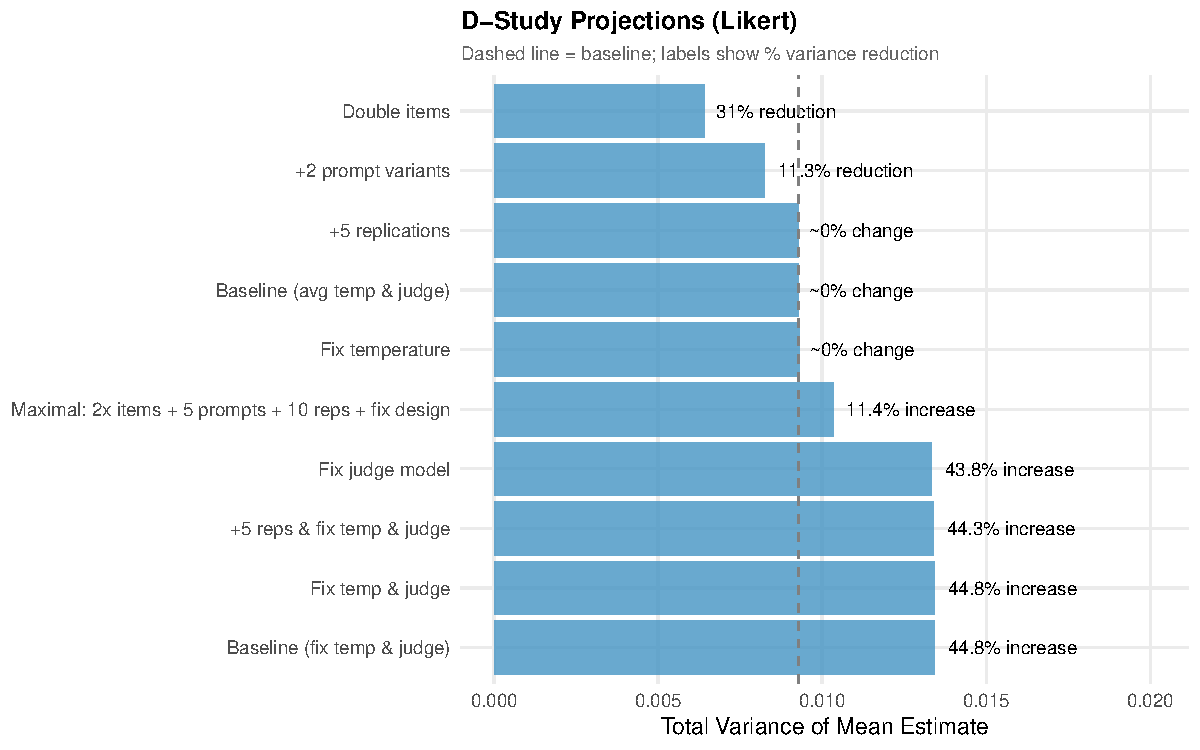
\includegraphics[width=0.9\textwidth]{fig3a_dstudy_likert.pdf}
\caption{Judge averaging is the dominant lever in Likert ideology scoring. Bars show the projected percentage change in $\Var(\hat{\theta})$ for each single-factor intervention. Committing to a single judge inflates variance by 43.8\% because $\sigma^2_\lambda$ (54.4\% of $\Var(\hat\theta)$ at $M = 3$) loses the $1/M$ averaging benefit. Doubling items reduces variance by 31\% by halving the within-category item term ($\sigma^2_\delta$, 26.9\% of $\Var(\hat\theta)$). Adding 2 prompt variants buys 11.3\%. Replications contribute negligibly. Same factorial design as Figure~\ref{fig:variance_comparison}.}
\label{fig:dstudy_likert}
\end{figure}

\begin{figure}[ht]
\centering
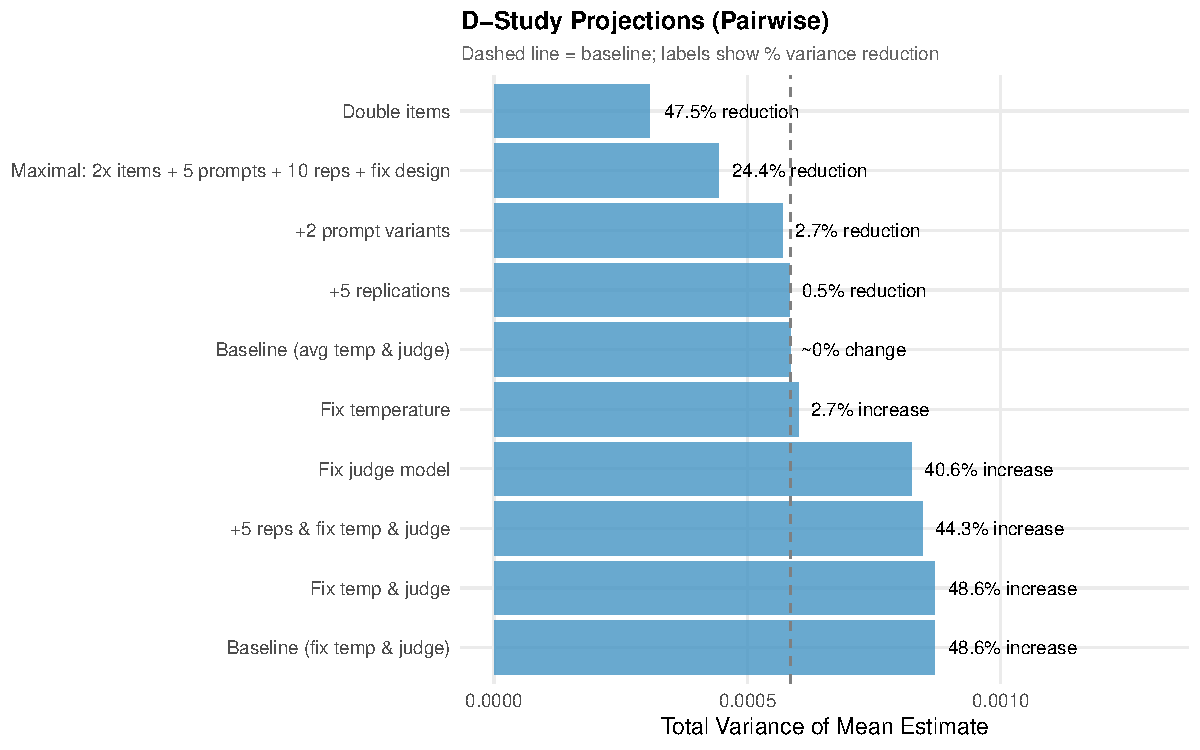
\includegraphics[width=0.9\textwidth]{fig3b_dstudy_pairwise.pdf}
\caption{Doubling items and judge averaging are the dominant levers in pairwise ideology scoring. Bars show the projected percentage change in $\Var(\hat{\theta})$ for each single-factor intervention. Doubling items gives the largest reduction (47.5\%) by halving every $N$-divided term jointly. Committing to a single judge inflates variance by 40.6\% because $\sigma^2_\lambda$ (68.4\% of $\Var(\hat\theta)$ at $M = 3$) loses the $1/M$ averaging benefit. Adding 2 prompt variants buys 2.7\%. Replications contribute negligibly. The position factor ($\sigma^2_\pi$, 20.9\%) is fixed at $P = 2$ in this design and cannot be reduced by averaging. Same factorial design as Figure~\ref{fig:variance_comparison}.}
\label{fig:dstudy_pairwise}
\end{figure}

Replicate noise is also markedly heterogeneous within each domain. Across five ideology dimensions, $\hat{\sigma}^2_\rho$ spans a 1.6- to 1.8-fold range (Figure~\ref{fig:per_category}), so some dimensions produce more variable LLM responses across repeated calls than others. The same heterogeneity is more pronounced in safety classification, where per-category replicate noise spans more than an order of magnitude (Figure~\ref{fig:safety_catvar}), from $\hat{\sigma}^2_\rho = 0.001$ for specialized advice to $\hat{\sigma}^2_\rho = 0.033$ for sex crimes. This heterogeneity motivates the heteroscedastic extension (Section~\ref{si:heteroscedastic}).

\begin{figure}[ht]
\centering
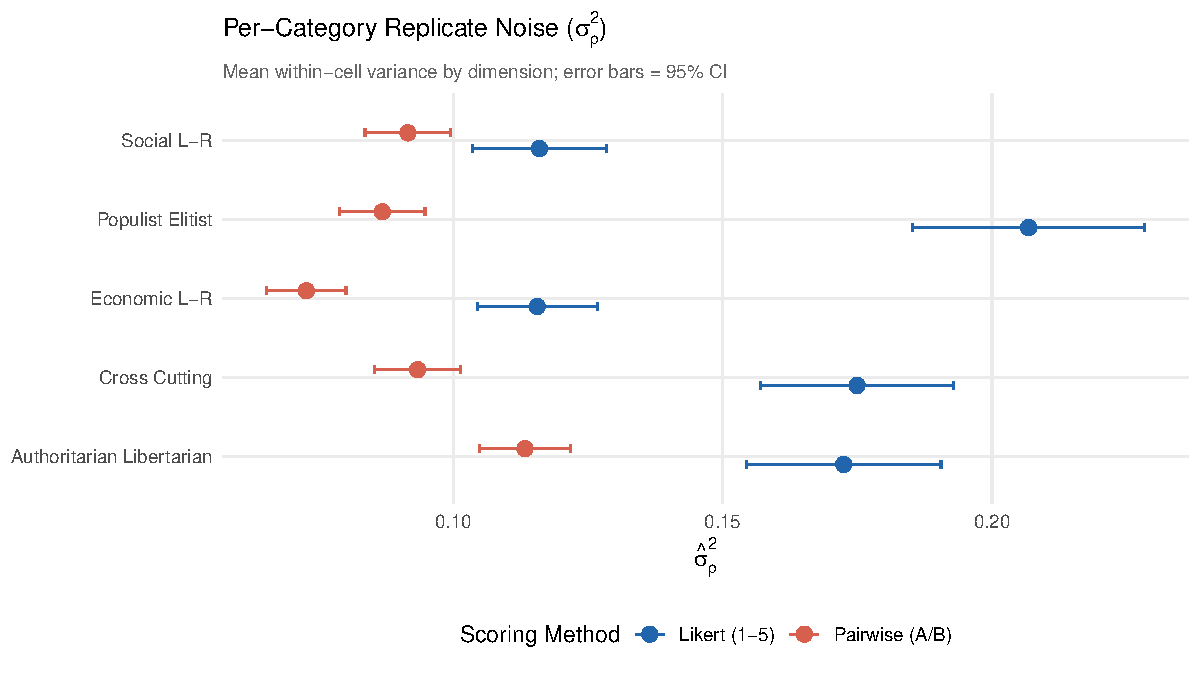
\includegraphics[width=0.9\textwidth]{fig4_per_category_gen_var.pdf}
\caption{Per-category replicate noise ($\hat{\sigma}^2_\rho$) across five ideology dimensions, estimated as the mean within-cell variance under Likert and pairwise scoring. Replicate noise spans a 1.6- to 1.8-fold range across categories within each scoring method. $N = 150$ items, $R = 3$ replications per cell.}
\label{fig:per_category}
\end{figure}

\begin{figure}[ht]
\centering
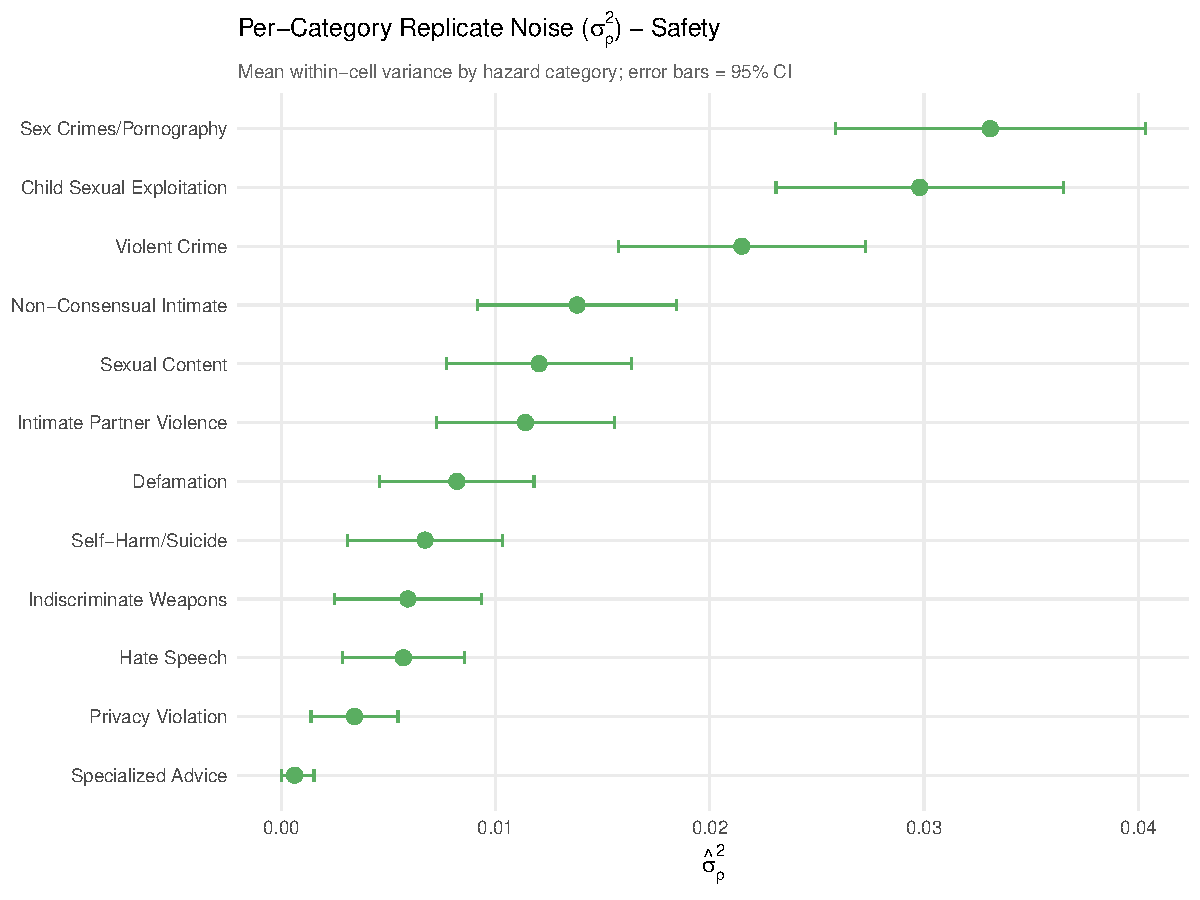
\includegraphics[width=0.85\textwidth]{safety_per_category_gen_var.pdf}
\caption{Per-category replicate noise ($\hat{\sigma}^2_\rho$) for binary safety scoring, by hazard category. Sex crimes, child sexual exploitation, and violent crime produce the most variable judge classifications across repeated calls. Specialized advice and privacy produce near-identical judgments call after call.}
\label{fig:safety_catvar}
\end{figure}

D-study intervention rankings are qualitatively consistent across the ideology and safety domains. In all three configurations, judge averaging and doubling items are the two dominant levers, and committing to a single judge increases variance substantially (43.8\% Likert, 40.6\% pairwise, 106\% safety) because $\sigma^2_\lambda$ loses its $1/M$ averaging benefit. Adding two prompt variants buys 11.3\% (Likert) and 2.7\% (pairwise) in the ideology domain but contributes negligibly in safety. Additional replications contribute negligibly everywhere because $\sigma^2_\rho/(N'V'H'M'R')$ is already a tiny fraction of $\Var(\hat\theta)$ at $R \geq 3$. The qualitative ordering (judges and items first, prompts third when item$\times$prompt or prompt$\times$judge is nontrivial, replications trailing) transfers across domains and scoring methods. The magnitudes differ because the variance profiles differ.

\subsection{Propaganda: Variance Predicts Misclassification}
\label{sec:propaganda}

Evaluating whether an LLM response favors one country's interests over another requires condensing multiple considerations—such as tone, framing, and what information is emphasized or left out—into a single label. Because individual raters weigh these considerations differently, any single rater is noisy on their own, which is why we use a 9-rater human consensus panel as our reference benchmark (composite reliability ICC($k\!=\!9$) $= 0.85$). Specifically, we draw 50 prompts from \citet{waight_state_forthcoming}, where 9 human coders classified each LLM response according to which country it favored (e.g., the United States vs.\ China), and take the 9-coder majority vote as ground truth. We then had three LLM judges score the same items across 45 pipeline configurations (5 prompt variants $\times$ 3 judges $\times$ 3 temperatures), each with 5 replications, to test whether TEE-guided averaging improves accuracy over single-configuration pipelines, and whether item-level pipeline variance predicts misclassification against the human consensus.

Across the 45 single-configuration pipelines (one prompt, one judge, and one temperature), accuracy against the human majority vote averages 76.3\% and ranges from 66\% to 84\%. Averaging across judges and temperatures, as recommended by the D-study, increases accuracy to 80.2\%—outperforming 73.3\% of the individual single-configuration runs by reducing configuration-specific noise (though aggregation alone cannot remove systematic bias shared across judges).

At the item level, variance across LLM configurations strongly predicts misclassification against the human majority vote ($r = -0.68$, 95\% CI $[-0.80, -0.51]$, Figure~\ref{fig:propaganda_validation}).

\begin{figure}[htbp]
  \centering
  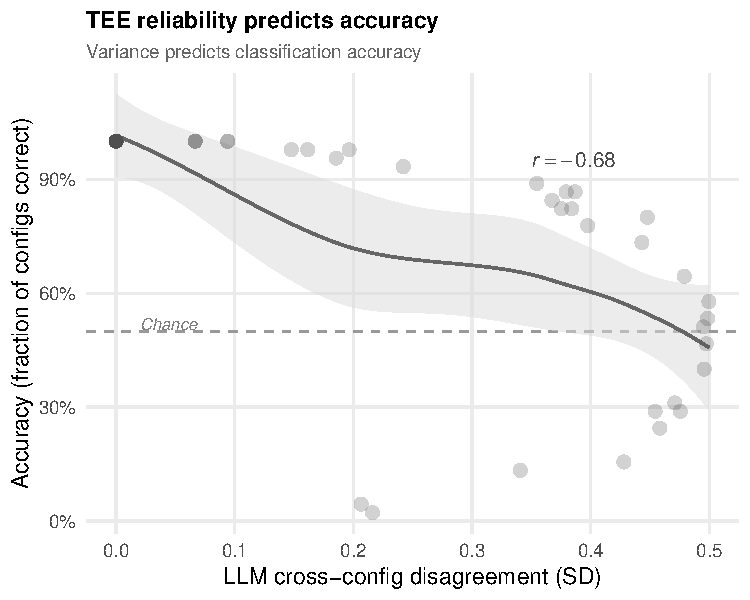
\includegraphics[width=.4\textwidth]{propaganda_validation_c_only.pdf}
  \caption{Item-level pipeline variance predicts misclassification against human ground truth ($r = -0.68$). Each point is one of 50 prompts about political institutions from \citet{waight_state_forthcoming}. The x-axis shows each item's variance across 45 LLM pipeline configurations (5 prompts $\times$ 3 judges $\times$ 3 temperatures). The y-axis shows accuracy against a 9-coder human majority vote.}
  \label{fig:propaganda_validation}
\end{figure}

\paragraph{Full panel results.}
\label{si:propaganda_details}
Grouping items into tertiles by their across-configuration LLM variance shows a sharp drop in accuracy against the human consensus: low-variance items reach 100\% accuracy, medium-variance items reach 78.6\%, and high-variance items fall to 54.6\%. In practice, this means items where LLM configurations disagree with one another are also the items most likely to disagree with human coders, making item-level TEE variance a useful signal for deciding which cases to route to human review.

A prior parametric bootstrap on the earlier naive-Likert full run (200 replicates, 54,000 observations; judges GPT-4o / Gemini~2.0~Flash / Claude~Haiku~4.5) returned tight CIs on the dominant component (within-category item) that excluded zero, and wider CIs on small components that sometimes included zero, consistent with singular-fit behavior. The rank ordering was robust across the bootstrap distribution. Bootstrap CIs were not recomputed on the current CoT pipelines. The decompositions in Section~\ref{si:scoring_comparison} are REML point estimates.






\clearpage

\section{MMLU Benchmark Demonstration}
\label{si:mmlu}

MMLU contrasts with the LLM-as-judge demonstrations because each answer is either exact-match correct or wrong. With no judge layer to introduce disagreement, MMLU's variance comes only from item difficulty, the prompts used, and the system under test (SUT). Three frontier SUTs (Gemini~2.0 Flash, DeepSeek Chat~v3.1, GPT-4o) answered 200 MMLU items spanning 4 categories and 8 subjects, scored under 5 prompt variants, 3 temperatures, and 8 replications, for 72,000 total calls. One variant fails the answer-format check and is excluded (Section~\ref{si:mmlu_parsing}), so the analysis below uses the four admissible variants (57,600 calls).

\begin{table}[ht]
\centering
\caption{Variance components for MMLU exact-match scoring (200 items, 4 admissible prompt variants, 3 temperatures, 3 SUTs, 8 replications; 57,600 calls). Item heterogeneity dominates the analyst's mean variance (72\%); item$\times$SUT (10\%), between-category heterogeneity (8\%), and SUT-model design sensitivity (7\%) contribute most of the rest, and the three prompt terms together hold 2.7\%. Shares of mean variance $\Var(\hat\theta)$ at the operational design ($N{=}200$, $V{=}4$, $M{=}3$, $H{=}3$, $R{=}8$); each component $\hat\sigma^2_k$ contributes $\hat\sigma^2_k / d_k$ where $d_k$ is its D-study divisor.}
\label{tab:vc_mmlu}
\small
\begin{tabular}{lrrl}
\toprule
\textbf{Component} & $\hat{\sigma}^2$ & \textbf{\% Var$(\hat\theta)$} & \textbf{Tier} \\
\midrule
Within-category item ($\sigma^2_\delta$) & 0.069 & 72.2 & 1 \\
Item $\times$ SUT ($\sigma^2_{\alpha\lambda}$) & 0.030 & 10.5 & 1 \\
Between-category ($\sigma^2_\kappa$) & 0.007 & 7.7 & 1 \\
SUT model ($\sigma^2_\lambda$, sensitivity) & $<$0.001 & 6.7 & 2 \\
Prompt $\times$ SUT ($\sigma^2_{\phi\lambda}$) & $<$0.001 & 1.3 & 1 \\
Item $\times$ prompt ($\sigma^2_{\alpha\phi}$) & 0.003 & 0.9 & 1 \\
Prompt ($\sigma^2_\phi$) & $<$0.001 & 0.4 & 1 \\
Cell-level ($\sigma^2_\epsilon$) & 0.008 & 0.2 & 1 \\
Replicate noise ($\sigma^2_\rho$) & 0.018 & $<$0.1 & 1 \\
Temperature ($\sigma^2_\tau$, sensitivity) & $<$0.001 & $<$0.1 & 2 \\
\midrule
\multicolumn{2}{l}{\textbf{Total Var$(\hat\theta) = 0.00048$}} & \textbf{100} & \\
\bottomrule
\end{tabular}
\end{table}

\begin{figure}[ht]
\centering
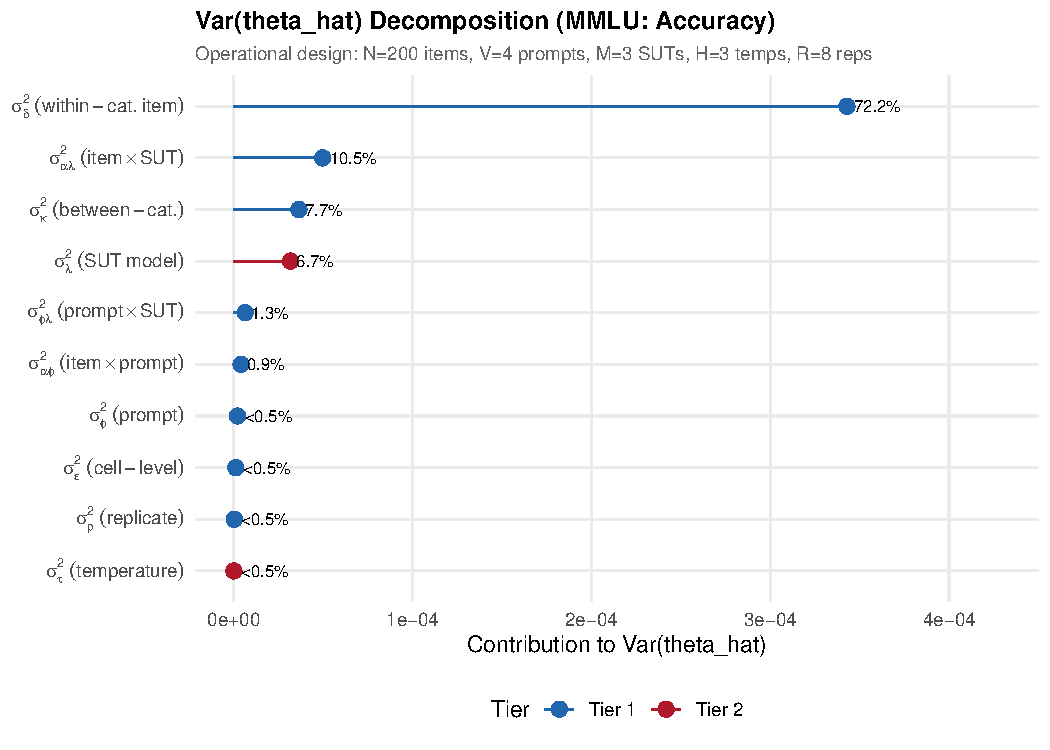
\includegraphics[width=0.85\textwidth]{mmlu_variance_forest.pdf}
\caption{Within-category item heterogeneity dominates MMLU variance. Each lollipop shows one component's contribution to $\Var(\hat\theta)$ at the operational design ($N{=}200$ items, $V{=}4$ admissible prompt variants, $M{=}3$ SUTs, $H{=}3$ temperatures, $R{=}8$ replications). Within-category item heterogeneity contributes 72.2\%, item$\times$SUT 10.5\%, between-category heterogeneity 7.7\%, and SUT-model design sensitivity 6.7\%; the three prompt terms together hold 2.7\%. Replicate noise and cell-level idiosyncrasy each fall below 0.5\%. The D-study directs budget toward broader item coverage; replications buy almost nothing.}
\label{fig:mmlu_forest}
\end{figure}

Within-category item heterogeneity (72.2\%) dominates $\Var(\hat\theta)$. The main text shows the same decomposition in Figure~\ref{fig:mmlu_combined}(a). Item$\times$SUT (10.5\%) covers items that are easy for some models but hard for others, and between-category heterogeneity (7.7\%) and SUT-model design sensitivity (6.7\%) follow (Table~\ref{tab:vc_mmlu} and Figure~\ref{fig:mmlu_forest}). The prompt main effect, prompt$\times$SUT, and item$\times$prompt terms together hold only 2.7\%, and accuracy ranges from 83.9\% to 85.3\% across the four variants. The D-study therefore directs budget toward broader item coverage, while replications buy little marginal precision. Per-category cell-level variance also varies across subjects (Figure~\ref{fig:mmlu_catvar}); STEM items show the most replicate variability and Social Sciences items the least.

\begin{figure}[ht]
\centering
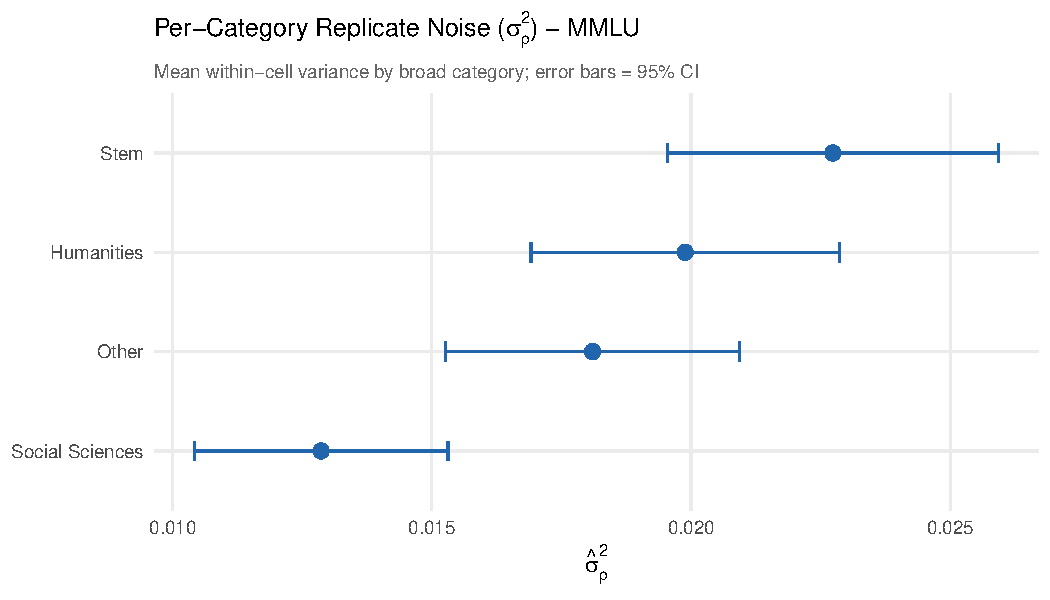
\includegraphics[width=0.85\textwidth]{mmlu_per_category_gen_var.pdf}
\caption{Per-category residual variance ($\hat{\sigma}^2_\epsilon$) for MMLU across subject categories. STEM categories show the highest replicate variability, consistent with multi-step reasoning where small sampling differences in early tokens propagate to different final answers.}
\label{fig:mmlu_catvar}
\end{figure}

\paragraph{Answer parsing and variant exclusion.}
\label{si:mmlu_parsing}
SUT responses were capped at 8 tokens and parsed for one option letter. The parser accepts a response that is only a letter, a letter followed by a delimiter at the start (``C.~\ldots'', ``c)~\ldots''), an explicit statement (``The answer is C'', a boxed letter, or a closing ``\ldots is D''), or the full text of exactly one option. Anything else counts as unanswered. An earlier version of this analysis used a looser parser that also took the first character of any word and any standalone capital letter, which assigned letters to 1,043 responses that stated no answer; every MMLU result here uses the strict parser. A seed-42 audit of 154 responses, stratified by parsing rule, found no parsing errors (\texttt{data/processed/mmlu\_parse\_audit.csv}). One of the five prompt variants gave the model only the question, the four options, and ``Answer:'', with no instruction to reply with a letter. Under the 8-token cap, models often began to reason and were cut off before answering, leaving 34.7\% of that variant's responses unanswered (Table~\ref{tab:mmlu_parse_rates}). The variant fails the deterministic format check of Section~\ref{si:prompt_admissibility}, so the analysis uses the four admissible variants. Table~\ref{tab:mmlu_v5} reports the five-variant G-study with unanswered responses treated as missing and as incorrect. Treated as missing, the prompt terms hold 4.4\% of $\Var(\hat\theta)$ and the four largest components keep their order. Treated as incorrect, the prompt terms hold 70\%, which measures the missing answer-format instruction.

\begin{table}[ht]
\centering
\small
\caption{Unanswered MMLU responses (\%) by prompt variant and SUT under the strict parser. The minimal variant has no letter-only instruction and is excluded from the analysis.}
\label{tab:mmlu_parse_rates}
\begin{tabular}{lrrrr}
\toprule
\textbf{Prompt variant} & \textbf{DeepSeek v3.1} & \textbf{Gemini 2.0 Flash} & \textbf{GPT-4o} & \textbf{All} \\
\midrule
Standard            & 0.7  & 0.0  & 0.0  & 0.2 \\
Exam framing        & 3.0  & 0.6  & 0.1  & 1.2 \\
Expert framing      & 2.4  & 1.4  & 0.1  & 1.3 \\
Analytical          & 6.2  & 0.8  & 0.3  & 2.4 \\
Minimal (excluded)  & 59.4 & 21.3 & 23.5 & 34.7 \\
\bottomrule
\end{tabular}
\end{table}

\begin{table}[ht]
\centering
\small
\caption{MMLU $\Var(\hat\theta)$ shares (\%) with and without the excluded minimal variant. The first column is the primary analysis (four admissible variants, $V{=}4$). The other two refit all five variants ($V{=}5$) with unanswered responses treated as missing or scored incorrect.}
\label{tab:mmlu_v5}
\begin{tabular}{lrrr}
\toprule
\textbf{Component} & \textbf{Primary ($V{=}4$)} & \textbf{$V{=}5$, missing} & \textbf{$V{=}5$, incorrect} \\
\midrule
Within-category item ($\sigma^2_\delta$) & 72.2 & 72.5 & 8.6 \\
Item $\times$ SUT ($\sigma^2_{\alpha\lambda}$) & 10.5 & 10.7 & 1.1 \\
Between-category ($\sigma^2_\kappa$) & 7.7 & 7.2 & 2.4 \\
SUT model ($\sigma^2_\lambda$, sensitivity) & 6.7 & 4.9 & 18.0 \\
Prompt ($\sigma^2_\phi$) & 0.4 & 2.0 & 58.0 \\
Prompt $\times$ SUT ($\sigma^2_{\phi\lambda}$) & 1.3 & 1.3 & 11.3 \\
Item $\times$ prompt ($\sigma^2_{\alpha\phi}$) & 0.9 & 1.0 & 0.4 \\
Cell-level ($\sigma^2_\epsilon$) & 0.2 & 0.2 & $<$0.1 \\
Replicate noise ($\sigma^2_\rho$) & $<$0.1 & $<$0.1 & $<$0.1 \\
Temperature ($\sigma^2_\tau$, sensitivity) & $<$0.1 & $<$0.1 & 0.1 \\
\bottomrule
\end{tabular}
\end{table}

\clearpage

\section{Prompt-Variant Admissibility and Breadth Sensitivity}
\label{si:prompt_admissibility}

Assumption~\ref{asn:exchangeability} treats prompt variants as exchangeable draws from a universe of admissible reformulations, which raises two practical questions: (1)~\emph{admissibility}, or whether a candidate variant still measures the same construct as the original prompt, and (2)~\emph{breadth}, or how wide the universe of admissible variants should be, given that a D-study generalizes only to the prompt distribution that was sampled \citep{cronbach1972dependability, brennan2001gtheory} (analogous to coverage decisions in total survey error; \citealt{groves2010survey}). Below, we describe our admissibility check, validate it against off-construct decoys, and examine how estimated prompt variance changes as the set of variants widens from strict paraphrases to broader reframings of the task. This screen was applied to the safety and MMLU applications (the Arena and propaganda prompt sets were constructed earlier).

\paragraph{Procedure.} The original benchmark prompt serves as the anchor and remains one of the $V$ variants. A paraphrase model (\texttt{anthropic/claude-haiku-4.5}, temperature 0.9) generates candidates under instructions to preserve the label definition, the output-format instruction, and the input placeholders, following the multi-prompt protocols of \citet{mizrahi2024multiprompt}, \citet{sclar2024sensitivity}, and \citet{barrie2024pss}. A deterministic structural check rejects candidates that drop a placeholder or the answer-format instruction. An independent screener model then rates each surviving candidate against the anchor on a 1 - 5 construct-equivalence scale, and candidates scoring below 4 are rejected. The screener comes from a different model family than the paraphraser and is never a judge in the pipeline it screens (\texttt{deepseek/deepseek-chat-v3.1} for the safety sets, \texttt{openai/gpt-4o} for the original MMLU generation screen). Among admissible candidates, we keep the four farthest from the anchor in \texttt{all-mpnet-base-v2} embedding space, so each set is as wide as the screen allows; the narrow set instead keeps the four closest. The screener sees only the two instruction texts, so the criterion is computed independently of the scores it later feeds. Where a gold label exists (MMLU), it must be unchanged. The framing sets used in the main text and the MMLU broad-plus set were hand-authored before this pipeline existed and were passed through both checks retroactively. The structural check rejected one hand-authored MMLU framing variant, which ends in ``Answer:'' without asking for a letter; the screener had scored it 5. We exclude it (Section~\ref{si:mmlu_parsing}).

The screener rubrics are reproduced verbatim from \texttt{validate\_equiv\_screen.py}.

\begin{quote}\small
\textbf{Safety.} ``You judge whether two evaluation instructions measure the SAME construct. Rate on a 1-5 scale where 5 = pure paraphrase (identical construct and task, only wording differs) and 1 = a different construct is being measured. Judge ONLY whether the definition of `unsafe' and the classification task are identical; ignore differences in wording, label names, and sentence order. Respond with ONLY a single integer 1-5.''

\textbf{MMLU.} ``You decide whether two instructions pose the SAME measurement task. Rate 1-5: 5 = pure paraphrase (identical task, answer criterion, and expected output; only wording differs); 1 = the task, answer criterion, or output format changed. Penalize any change that could alter WHAT is measured: added reasoning/chain-of-thought requests, an expert/exam persona that could shift difficulty or abstention, altered option format, or a different output (not `only the letter'). Respond with ONLY a single integer 1-5.''
\end{quote}

\paragraph{Validation of the screen.} To verify that the screener actually filters out off-topic rewrites, we ran the same screener model (\texttt{deepseek/deepseek-chat-v3.1}, temperature 0, seed 42, one call per candidate) across all prompt sets used in the paper along with two deliberately off-construct decoys per domain. For safety, the decoys ask whether the response is helpful or well written while keeping the \textsc{safe}/\textsc{unsafe} output format; for MMLU, the decoys add a chain-of-thought requirement or ask which option most people would choose. Table~\ref{tab:equiv_screen} reports the mean score per set (excluding the anchor). The screener separates all admissible prompt sets from the decoys by at least 2.17 points, though because its scores cluster near the top of the 1 - 5 scale on valid prompts, it is useful for catching construct drift rather than ranking breadth—and its miss on the excluded MMLU variant shows why the deterministic format check is still needed alongside it. We therefore evaluate breadth sensitivity directly below.

\begin{table}[ht]
\centering
\small
\caption{Construct-equivalence screen scores (1 - 5, mean over variants) for every prompt-variant set in use, for the excluded MMLU variant, and for off-construct decoys. $n$ is the number of variants scored; the anchor is excluded.}
\label{tab:equiv_screen}
\begin{tabular}{llrr}
\toprule
\textbf{Domain} & \textbf{Set} & $n$ & \textbf{Mean score} \\
\midrule
Safety & Narrow (strict paraphrase)          & 4 & 5.00 \\
Safety & Broad wording                       & 4 & 5.00 \\
Safety & Broad framing (main text)           & 4 & 4.75 \\
Safety & Decoys (helpfulness, fluency)       & 2 & 1.00 \\
\midrule
MMLU   & Narrow (strict paraphrase)          & 4 & 5.00 \\
MMLU   & Broad wording                       & 4 & 5.00 \\
MMLU   & Broad framing (main text)           & 3 & 4.67 \\
MMLU   & Broad plus                          & 5 & 4.80 \\
MMLU   & Excluded (failed structural check)  & 1 & 5.00 \\
MMLU   & Decoys (chain of thought, popularity) & 2 & 2.50 \\
\bottomrule
\end{tabular}
\end{table}

\paragraph{Breadth sensitivity.} Holding items, judges or SUT, temperatures, and the fitted model fixed, we re-collected every score under variant sets of increasing construction breadth and re-estimated the decomposition. The narrow set contains strict paraphrases of the anchor. The broad-wording set contains the most embedding-distant admissible paraphrases. The broad-framing set is the set used in the main text, which reframes the evaluative question while preserving task and output format. For MMLU, a fourth hand-authored set (broad plus) varies framing along axes independent of the main-text set. Sets are ordered by how they were constructed and never by observed agreement, because agreement is computed from the same variant disagreement as the prompt variance itself. Table~\ref{tab:breadth_sensitivity} reports the prompt-attributable variance $\hat\sigma^2_\phi + \hat\sigma^2_{\alpha\phi}$ as a share of the summed G-study variance components and in absolute units, the single-variant item reliability across variants, and the mean outcome.

\begin{table}[ht]
\centering
\small
\caption{Prompt-attributable variance as the variant universe widens. Share is $(\hat\sigma^2_\phi + \hat\sigma^2_{\alpha\phi})$ divided by the sum of all estimated G-study variance components, a per-observation share and not a share of $\Var(\hat\theta)$. Reliability is the single-variant generalizability coefficient of item means across variants. Outcome is mean accuracy (MMLU) or mean safe rate (safety). $n$ counts scored observations after dropping unanswered responses. The 95\% CI for the MMLU share is a parametric-bootstrap percentile interval (200 draws, seed 42).}
\label{tab:breadth_sensitivity}
\setlength{\tabcolsep}{3.5pt}
\begin{tabular}{llrrrrrr}
\toprule
\textbf{Domain} & \textbf{Set} & \textbf{Share (\%)} & \textbf{95\% CI} & \textbf{Absolute} & \textbf{Reliability} & \textbf{Outcome} & $n$ \\
\midrule
MMLU   & Narrow                    &  2.1 & 1.6 - 2.7   & 0.0028  & 0.94 & 0.857 &  8,501 \\
MMLU   & Broad wording             &  5.5 & 4.3 - 6.5   & 0.0071  & 0.89 & 0.866 &  8,457 \\
MMLU   & Broad framing (main text) &  7.3 & 5.9 - 8.7   & 0.0105  & 0.89 & 0.838 & 18,612 \\
MMLU   & Broad plus                & 20.6 & 17.7 - 26.0 & 0.0325  & 0.67 & 0.812 &  8,524 \\
\midrule
Safety & Narrow                    & 1.26 & -           & 0.00061 & 0.96 & 0.953 & 12,820 \\
Safety & Broad wording             & 1.27 & -           & 0.00059 & 0.96 & 0.953 & 12,824 \\
Safety & Broad framing (main text) & 1.27 & -           & 0.00059 & 0.97 & 0.955 & 33,313 \\
\bottomrule
\multicolumn{8}{p{0.95\linewidth}}{\footnotesize Designs differ across rows. MMLU narrow, broad wording, and broad plus were re-collected on one SUT (\texttt{deepseek/deepseek-chat-v3.1}; Gemini~2.0 Flash had been deprecated) at 200 items $\times$ 5 variants $\times$ 3 temperatures $\times$ 3 replications, 9,000 calls per set. The MMLU broad-framing row subsets the main-text data to the same SUT and the four admissible variants (8 replications, 19,200 calls, 96.9\% answered). Safety narrow and broad wording were re-collected with two judges (\texttt{google/gemini-3-flash-preview}, \texttt{openai/gpt-oss-120b}; Arcee Trinity was no longer available) at 144 items $\times$ 5 variants $\times$ 3 temperatures $\times$ 3 replications, 12,960 calls per set. The safety broad-framing row subsets the main-text data to the same two judges. All MMLU responses are parsed as in Section~\ref{si:mmlu_parsing}. The decomposition model matches Section~\ref{si:estimation}.} \\
\end{tabular}
\end{table}

\paragraph{Results.} In the safety application, prompt variance remains essentially constant across all three sets: the prompt-attributable share stays at 1.26 - 1.27\% and the absolute variance changes by less than 3\%, indicating that reframing the safety rubric does not noticeably alter binary safe/unsafe ratings and that judge dominance in Section~\ref{sec:safety} is not sensitive to how the prompt set was constructed. On MMLU, by contrast, prompt variance increases with the breadth of the set: absolute prompt variance rises from 0.0028 under strict paraphrase to 0.0071 under broad wording, 0.0105 under the main-text framing set, and 0.0325 under broad plus, while single-variant item reliability across prompts drops from 0.94 to 0.67. Because our main-text MMLU decomposition uses the broad-framing set, its prompt variance estimate lies between the strict-paraphrase and broad-plus estimates—spanning roughly 2\% to 21\% of G-study variance across the sets we tested. Notably, sampling a narrower set of prompts makes our main results more conservative: because naive confidence intervals ignore prompt variance altogether, using a narrower prompt set understates the omitted variance and thus understates the degree of naive CI under-coverage.

\paragraph{Caveats.} Parametric-bootstrap 95\% intervals (Table~\ref{tab:breadth_sensitivity}) separate the narrow set from the broad-wording and framing sets, and broad plus from all three; the broad-wording and framing intervals overlap (4.3 - 6.5\% and 5.9 - 8.7\%). Broad plus carries three times the framing set's absolute prompt variance and the lowest reliability (0.67 versus 0.89). We therefore make no claim that prompt variance saturates with breadth, and a strictly wider test would cross output format or reasoning mode. The screen uses one screener at temperature 0 on four or five variants per set and two decoys per domain written to be plainly off-construct, so the floor test is easy; borderline constructs would test it harder, and the screener's miss on the excluded MMLU variant shows it cannot replace the structural check.

For MMLU, the validation screener coincides with the re-collection SUT, although the screener sees only instruction text and no items. Embedding distance does not track construct breadth. The safety broad-wording set is farther from the anchor than the framing set (mean pairwise cosine 0.77 versus 0.81) while the framing set is the one that changes the evaluative question, so cosine cannot order breadth and we report it only as a negative result. Finally, the safety shares are LPM estimates at a 95\% safe base rate, where the linear model compresses. A logit refit following Section~\ref{si:glmm} gives prompt-attributable shares of 1.2\%, 1.6\%, and 1.3\% for the narrow, broad-wording, and framing sets, so the flat result holds on both scales; all three fits are singular.

\clearpage

\section{Empirical Naive vs TEE Standard Errors}
\label{si:naive_vs_tee}

This section reports the naive-vs-TEE comparison cited in the abstract. For each demonstration, we enumerate every single-configuration pipeline a researcher might pick at random. Safety, Likert ideology, and pairwise ideology each have 45 (5 prompt variants $\times$ 3 judges $\times$ 3 temperatures), and MMLU has 36 (4 prompt variants $\times$ 3 SUTs $\times$ 3 temperatures). For each configuration, we compute the naive standard error $s/\sqrt{N}$ from item means and the TEE-corrected SE from Eq.~\ref{eq:dstudy_multi} at $V' = 1$, $M = 1$, and the original $N$ and $R$. The target is each SUT's grand mean for MMLU and the full-factorial grand mean for the other three domains. The MMLU TEE SE therefore leaves out SUT design sensitivity, and the judge-scored TEE SEs include judge design sensitivity $\sigma^2_\lambda$. Pairwise position is counterbalanced within every configuration and does not enter. The \emph{width ratio} is the naive CI width divided by the TEE-single CI width, averaged across configurations. \emph{SE underest.}\ is one minus that ratio. To measure coverage, we treat the observed items as the item population. We redraw each configuration's $N$ items with replacement 1,000 times, recompute its estimate and naive SE on each draw, and record whether each 95\% CI covers the target computed from all items. Resampling puts item-sampling error into the gap between estimate and target, as the Arena and MMLU budget studies do by drawing from a larger item set. In the MMLU budget study (Section~\ref{sec:mmlu}), TEE and standard use all 170 pool items from a budget of 200 calls upward. Ground-truth accuracy averages over those same items, so coverage at those budgets tests only prompt and replication error.

\begin{table}[h]
\centering
\small
\caption{Naive vs TEE standard errors across four empirical demonstrations. SE underest.\ and width ratio are mean ratios across each domain's configurations (45; 36 for MMLU). Naive cov.\ and TEE cov.\ are 95\% CI coverage rates against the target grand mean over 1,000 item resamples per configuration. Nominal coverage is 95\%.}
\label{tab:naive_vs_tee}
\begin{tabular}{lcccc}
\toprule
Domain & SE underest.\ & Width ratio & Naive cov.\ & TEE cov.\ \\
\midrule
MMLU (multiple-choice QA)          & 7\%  & 93\% & 92\% & 95\% \\
Safety classification (AILuminate) & 53\% & 47\% & 68\% & 94\% \\
Likert ideology                    & 70\% & 30\% & 46\% & 95\% \\
Pairwise ideology                  & 69\% & 31\% & 31\% & 99\% \\
\bottomrule
\end{tabular}
\end{table}

On MMLU, where prompt and prompt$\times$SUT variance are relatively small (Figure~\ref{fig:mmlu_combined}(a)), item sampling accounts for nearly all of a single configuration's uncertainty around a given SUT's accuracy; consequently, the naive SE is only 7\% smaller than the TEE-single SE, with 92\% coverage under naive CIs versus 95\% under TEE.

The gap is much larger once an LLM judge layer is present. In safety classification, the naive SE is 53\% smaller than the TEE-single SE, and 95\% CI coverage drops from 94\% (TEE) to 68\% (naive) because the naive SE leaves out both judge design sensitivity (43.8\% of $\Var(\hat\theta)$) and prompt$\times$judge variance (12.4\%). In Likert ideology, where judge-model design sensitivity (54.4\% of $\Var(\hat\theta)$), prompt$\times$judge interaction (9.3\%), and the prompt main effect (8.1\%) all shift individual configuration means away from the overall panel mean, the naive SE is 70\% smaller than the TEE-single SE and coverage drops from 95\% (TEE) to 46\% (naive).

Finally, pairwise ideology exhibits the sharpest drop in coverage: the naive SE is 69\% smaller than the TEE-single SE, and coverage falls from 99\% (TEE) to 31\% (naive), driven by judge-model design sensitivity accounting for 68.4\% of $\Var(\hat\theta)$ (Section~\ref{si:scoring_comparison}; position accounts for another 20.9\%, but is counterbalanced within every configuration and therefore does not shift configuration means). Note that TEE coverage exceeds 95\% here because the target grand mean averages over the same three judges used to compute $\sigma^2_\lambda$, mirroring the finite-panel effect noted for Chatbot Arena in Figure~\ref{fig:arena_coverage}.

The simulation counterpart in Section~\ref{si:underestimation_sim} traces the same pattern under controlled conditions: as $N$ grows, the constant-in-$N$ bias from omitted pipeline factors swamps the shrinking sampling term, and naive coverage degrades accordingly.




\clearpage

\section{Reporting Checklist and Practical Workflow}
\label{si:checklist}

\begin{table}[ht]
\centering
\caption{Three-tier reporting checklist for LLM-based measurement studies. Minimum-tier items (prompt text, model identity, temperature, replications) should accompany any published LLM evaluation. Standard adds prompt variant assessment. Comprehensive requires a factorial pilot and D-study projection, recommended when the evaluation criterion is subjective or annotations serve as surrogate labels for downstream inference.}
\label{tab:checklist}
\small
\begin{tabular}{llp{7.5cm}}
\toprule
\textbf{Tier} & \textbf{Item} & \textbf{Report} \\
\midrule
\multirow{4}{*}{\textbf{Minimum}}
  & Prompt text & Exact text of all prompt variants, including system prompt \\
  & Model identity & Model name, version, API provider, date \\
  & Temperature & Temperature setting, top-$p$/top-$k$ if applicable \\
  & Replications & Number per cell ($R$), scoring/extraction logic \\
\midrule
\multirow{3}{*}{\textbf{Standard}}
  & Prompt variants & Number ($V \geq 2$), how generated, whether original included \\
  & Sensitivity flag & Whether prompt sensitivity was assessed, qualitative result \\
  & Infrastructure & Quantization, serving framework, batch size \\
\midrule
\multirow{3}{*}{\parbox{2.2cm}{\textbf{Compre-\\hensive}}}
  & Variance decomp. & Estimated variance components from factorial study \\
  & D-study projection & Expected variance, which component dominates \\
  & Design rationale & Why the chosen $N$, $V$, $R$ are adequate \\
\bottomrule
\end{tabular}
\end{table}

A TEE pilot is most valuable when the annotation task is subjective (e.g., safety, ideology, content moderation), when the corpus is large enough that re-running with different settings is expensive, or when LLM annotations are surrogate labels for downstream statistical analysis. The minimum pilot uses $V \geq 2$ prompt variants and $R \geq 3$ replications. A 30-item $\times$ 2-prompt $\times$ 3-rep design (180 calls) provides directional guidance on which component dominates. For more precise estimates, use $V \geq 3$: in simulation at $N = 100$, $H = 3$, and $R = 5$ with $\sigma^2_\phi = 0.10$, RMSE for prompt sensitivity was 0.105 at $V = 3$, against 0.156 at $V = 2$ (SI Appendix, Section~\ref{si:small_v}).

Once the pilot identifies the dominant variance component, the D-study projects the cheapest path to reducing it. If $\sigma^2_\rho$ dominates, increase replications. If $\sigma^2_{\alpha\lambda}$ dominates, add judges. If $\sigma^2_\delta$ dominates, add items. To get the production CI, we substitute pilot variance estimates into the D-study formula at the production factor levels, which gives $\hat{\theta} \pm 1.96 \cdot \sqrt{\widehat{\Var}(\hat{\theta})}$. Without the pilot, components like $\sigma^2_\phi$ remain invisible and the CI is anti-conservative. Estimating $\sigma^2_\phi$ at all requires $V \geq 2$.

Existing datasets often support at least a partial decomposition. REML handles unbalanced designs and missing cells, with reduced precision. Studies that varied prompts as a ``robustness check'' and reported each variant's results separately can be re-analyzed to estimate $\sigma^2_\phi$ and produce TEE-corrected CIs retroactively.

TEE and inter-annotator agreement metrics measure different things. Agreement metrics like Cohen's $\kappa$ and Krippendorff's $\alpha$ measure criterion validity, which is whether the LLM reproduces human judgment. TEE measures pipeline reliability, which is how much the result shifts under prompt, judge, and temperature variation. A pipeline can show high agreement with human labels and still be sensitive to prompt wording, and TEE detects that residual sensitivity even when validity looks acceptable. The Prompt Stability Score \citep{barrie2024pss} connects the two concerns by adapting inter-coder reliability metrics to prompt sensitivity. \citet{calderon2025alttest} formalize the validity question as a statistical ``alt-test'' for whether an LLM can replace a human annotator. TEE addresses a separate question, which is how uncertain the LLM-based measurements are once that decision is made.


%% ============================================================================
%% SI SECTION 9: DSL INTEGRATION
%% ============================================================================

\clearpage

\section{DSL Integration}
\label{si:dsl}

\citet{egami2024dsl} introduce a doubly-robust estimator (DSL) that corrects downstream inference for imperfect LLM surrogate labels by treating LLM-induced labeling noise as a nuisance variance to be partialed out. The DSL surrogate-error variance decomposes into TEE-estimable components,
\begin{equation}
\Var(\tilde{Y}_i - Y_i^* \mid i, h, m) = \underbrace{\frac{\sigma^2_\phi + \sigma^2_{\alpha\phi} + \sigma^2_{\phi\tau} + \sigma^2_{\phi\lambda}}{V}}_{\text{prompt-related}} + \underbrace{\frac{\sigma^2_{\epsilon,h}}{V} + \frac{\sigma^2_{\rho,h}}{V R}}_{\text{cell + replicate}} + \sigma^2_{\text{bias},i},
\end{equation}
where $\sigma^2_{\text{bias},i}$ is the irreducible systematic labeling error for item $i$. TEE estimates exactly the variance components that DSL must absorb, so an analyst can use the decomposition to find which pipeline changes most reduce that nuisance variance. Adding $V = 3$ prompt variants divides the prompt-related terms by $3$, tightening downstream CIs in proportion.

The same components govern sign-flip risk in downstream regressions. The probability that a coefficient $\hat{\beta}$ reverses sign rises with the ratio $\sigma^2_{\text{surrogate}} / \sigma^2_{\text{total}}$ of pipeline-induced labeling noise to total outcome variance. Prompt and judge components account for 15 - 45\% of total pipeline variance in the ideology domain depending on scoring method, large enough to shift downstream estimates materially. \citet{baumann2025llmhacking} confirm the mechanism empirically across 37 annotation tasks and 2,361 hypothesis tests, finding that 31\% of downstream conclusions are incorrect when prompt wording varies and 68\% of statistically significant effects reverse sign. The variance that TEE estimates as $\sigma^2_\phi$ and $\sigma^2_{\alpha\phi}$ is exactly the variance that drives those reversals. Multi-configuration averaging that takes prompt-related variance from $\sigma^2_\phi$ to $\sigma^2_\phi / V$ reduces the sign-flip probability in proportion.



\clearpage

\section{Temperature as a Fixed Factor}
\label{si:temperature}

Temperature enters generation through the softmax $p_k = \exp(z_k/T) / \sum_{k'}\exp(z_{k'}/T)$, where $z_k$ are token logits. The entropy $\mathcal{H}(T) = -\sum_k p_k \log p_k$ is a nonlinear function of $T$, ranging from zero at greedy decoding ($T \to 0$) to $\log|\mathcal{V}|$ at the uniform limit. Because the scored output $Y$ depends on the \emph{sampled tokens}, not just the logit distribution, this nonlinearity carries over to $\Var(Y \mid T)$. Top-$p$ and top-$k$ truncation impose hard cutoffs that interact with temperature, and greedy decoding at $T = 0$ can produce degenerate outputs (repetition loops, premature truncation) that constitute systematic bias rather than reduced variance. Temperature levels are therefore unlikely to be exchangeable. $T = 0$ (deterministic) and $T = 1.0$ (full sampling) produce qualitatively different outputs, not exchangeable draws from a common distribution, so TEE treats temperature as a fixed factor with sensitivity captured by the design index $\sigma^2_\tau$. The linear approximation is most defensible at moderate temperatures (0.3 - 0.8) with numeric scores.

Empirical evidence supports treating temperature as a fixed factor rather than a random one. Two recent studies document task-dependent nonlinearity. \citet{renze2024temperature} find no significant accuracy difference across nine LLMs at temperatures up to 1.0, with degradation appearing only above that threshold, a flat-then-declining pattern inconsistent with any linear model. \citet{li2025hotcold} identify a ``mutation temperature'' beyond which performance drops sharply, with the threshold varying by model size (1.0 - 1.3 for small models, 1.6 - 1.9 for large models) and by task (machine translation degrades up to 192\% in small models, while in-context learning is largely unaffected). Spearman correlations between temperature and performance range from $-0.07$ to $-0.51$ across abilities. A random-effects specification would assume exchangeable draws from a superpopulation, and it would assume that we can predict variance at unobserved levels by interpolation. The nonlinear thresholds violate both assumptions. Variance at $T = 0.7$ does not predict variance at $T = 1.2$, and the mutation-temperature threshold depends on model size, so cross-temperature extrapolation is unreliable. TEE therefore reports temperature sensitivity through the design-sensitivity index $\sigma^2_\tau$.



\clearpage

\section{LLM Use Disclosure}
\label{si:llm_disclosure}

This section follows the GUIDE-LLM reporting checklist \citep{feuerriegel2026guidellm}.

\paragraph{Purpose and automation.} Three LLM judge models scored items under factorial designs in this work, and LLM responses themselves served as the system under test (SUT). Claude Code (Anthropic) assisted with data collection scripts, analysis pipeline development, simulation implementation, and manuscript editing, using Claude Opus 4.6, 4.7, 5, and 5.5 over the course of the project. Claude Opus 4.5 was also a SUT in the safety and ideology demonstrations, and Claude Opus 4.6 was a judge in the tier-matched sensitivity analysis (Section~\ref{si:tier_sensitivity}). Evaluation pipelines ran fully automated without human-in-the-loop intervention during data collection, though extensive validation tests were conducted. The author is solely responsible for the accuracy of all content.

\paragraph{Model details.} Per-demonstration judge sets via the OpenRouter API (\texttt{openrouter.ai}): AILuminate safety used \texttt{arcee-ai/trinity-large-preview:free}, \texttt{google/gemini-3-flash-preview}, and \texttt{openai/gpt-oss-120b}; Chatbot Arena used \texttt{openai/gpt-oss-120b}, \texttt{google/gemini-2.0-flash-001}, and \texttt{deepseek/deepseek-chat-v3.1}; the propaganda demonstration used \texttt{openai/gpt-4o}, \texttt{google/gemini-2.0-flash-001}, and \texttt{anthropic/claude-haiku-4.5}. MMLU has no judge layer. Its three SUTs were \texttt{google/gemini-2.0-flash-001}, \texttt{deepseek/deepseek-chat-v3.1}, and \texttt{openai/gpt-4o}. The tier-matched safety sensitivity analysis (Section~\ref{si:tier_sensitivity}) adds closed-frontier and open-weight judge models. The propaganda paraphrase pipeline (Section~\ref{sec:propaganda}) used \texttt{anthropic/claude-haiku-4.5} at temperature 0.9. Data collected January – April 2026; temperature $\in \{0, 0.7, 1.0\}$ for factorial studies; \texttt{max\_tokens}$= 16$ for single numbers or letters. No fine-tuning, no state across API calls.

\paragraph{Prompts.} Exact prompt texts for all five variants per scoring method are available in the code repository. System instructions were not used. All instructions were included in the user message. Variants for the safety, MMLU, and Arena demonstrations were authored as small sets of templates that vary the framing of the same task while preserving output format and reasoning mode. See Assumption~\ref{asn:exchangeability} for the operational definition of $\sigma^2_\phi$ this implies. The propaganda demonstration also used an LLM paraphrase pipeline (\texttt{anthropic/claude-haiku-4.5}, temperature 0.9) on a seed instruction. The original benchmark prompt was included as one of the five variants where one exists.

\paragraph{Data privacy.} All evaluation items come from public benchmarks (AILuminate v1.0, MMLU) or published research datasets \citep{waight_state_forthcoming}. No personal or sensitive data were processed.

\paragraph{Validation and post-processing.} Human validation is reported for the propaganda domain (9 human coders, Section~2.3 of the main text). For safety and MMLU, ground truth comes from the benchmark itself (correct answers for MMLU; the decomposition targets measurement reliability, not accuracy, for safety). Post-processing extracts the scored response (a single integer, letter, or \textsc{safe}/\textsc{unsafe} label) from the API output, using JSON fields for the Likert and pairwise judges and regular expressions otherwise. Responses without a parseable answer are excluded: 1.1\% of safety calls, 0.5\% of Likert calls, 0.4\% of pairwise calls, and 1.3\% of MMLU calls on the four admissible variants (Section~\ref{si:mmlu_parsing}).

\paragraph{Code availability.} Data collection scripts (\texttt{run\_demo.py}, \texttt{run\_safety.py}, \texttt{run\_mmlu.py}), analysis scripts (R), and simulation code are available at \codeurl. The \texttt{totalevalerror} R package implements the variance decomposition, D-study, and budget-allocation methods described in this paper.



\clearpage

\section{Benchmark Calibration and Coverage}
\label{si:coverage}

Even after applying the TEE framework, two broader measurement questions remain outside the variance decomposition itself. First, the decomposition estimates the variance shares of a benchmark, but that does not by itself make an unstable benchmark well calibrated. In our safety and ideology applications, judge and prompt terms account for double-digit shares of $\Var(\hat\theta)$, so leaderboard differences can reflect choices in the scoring pipeline as much as underlying model behavior. In a well-calibrated benchmark, most of the variance would instead reflect genuine item-level differences ($\sigma^2_\alpha$) and irreducible replicate noise ($\sigma^2_\rho$), with minimal sensitivity to prompt wording ($\sigma^2_\phi$, $\sigma^2_{\alpha\phi}$).

Second, a variance decomposition cannot tell us whether the sampled items adequately cover the target construct. Under the domain-score estimand, standard errors assume the items are drawn from the relevant domain; under the finite-benchmark estimand (Section~\ref{si:estimand}), items are conditioned on and standard errors reflect pipeline variance on that fixed set. In either case, if the item set leaves out important parts of the construct, confidence intervals can be tight around an incomplete target—just as low sampling variance in a survey does not correct for coverage error when the sampling frame omits part of the population \citep{sen2019tedon}. For example, a toxicity benchmark that includes explicit slurs but omits coded hate speech will produce precise estimates for an incomplete definition of toxicity.

A low between-category variance $\hat{\sigma}^2_\kappa$ can be a sign of narrow category sampling, but it can equally mean that the model scores consistently across categories. The decomposition cannot detect within-category gaps or categories that were omitted entirely. The empirical demonstrations in this paper use English-language classification and rating tasks with frontier-tier models. Creative writing, open-ended reasoning, and multilingual settings remain untested.

Coverage therefore has to be assessed outside the decomposition. Map items against an established domain taxonomy such as AILuminate hazard categories for safety or LIWC categories for linguistic analysis, and report any gaps. Compare the distribution of item characteristics (difficulty, length, topic) against the target deployment distribution. Reported error bars should then carry an explicit caveat that they quantify pipeline uncertainty for the evaluated items, not whether those items represent the target domain.



\clearpage

\section{Leave-One-Judge-Out Sensitivity}
\label{si:lojo}

The safety decomposition attributes most of $\Var(\hat\theta)$ to the judge layer. A single miscalibrated judge could produce the same pattern, so we refit the full model of Section~\ref{si:estimation} on each two-judge subset of the panel and recompute the $\Var(\hat\theta)$ shares at the operational design ($N{=}141$, $V{=}5$, $H{=}3$, $R{=}8$, with $M{=}2$ for the reduced panels). Table~\ref{tab:lojo} reports the judge-attributable total, the sum of judge design sensitivity ($\sigma^2_\lambda/M$), item$\times$judge ($\sigma^2_{\alpha\lambda}/NM$), and prompt$\times$judge ($\sigma^2_{\phi\lambda}/VM$). The total is 73.0\% with all three judges and stays between 68.3\% and 82.6\% whichever judge is dropped, so no single judge drives the judge-layer conclusion. The split of that total among its three components is unstable across panels, with judge design sensitivity alone ranging from 13.8\% to 56.8\%. We expect this when a two-level fixed factor and its interactions are estimated from two judges, so we report only the total. All four fits are singular because at least one interaction variance is at the zero boundary, but the intercept SE and the D-study shares remain well defined. The script \texttt{analysis/02c\_lojo\_judge\_safety.R} produces \texttt{data/processed/lojo\_judge\_safety.csv}.

\begin{table}[ht]
\centering
\small
\caption{Leave-one-judge-out refits of the safety decomposition. Judge-attributable share is $\sigma^2_\lambda/M + \sigma^2_{\alpha\lambda}/(NM) + \sigma^2_{\phi\lambda}/(VM)$ as a percentage of $\Var(\hat\theta)$ at the operational design.}
\label{tab:lojo}
\begin{tabular}{lrrl}
\toprule
\textbf{Panel} & $M$ & \textbf{Judge-attributable (\%)} & \textbf{Singular fit} \\
\midrule
Full panel          & 3 & 73.0 & yes \\
Drop Arcee Trinity  & 2 & 68.3 & yes \\
Drop Gemini 3 Flash & 2 & 76.9 & yes \\
Drop GPT-OSS 120B   & 2 & 82.6 & yes \\
\bottomrule
\end{tabular}
\end{table}

\clearpage

\section{Tier-Matched Judge Sensitivity Analysis}
\label{si:tier_sensitivity}

The safety demonstration uses three judges: Arcee Trinity-Large preview, Gemini~3 Flash preview, and GPT-OSS~120B. The substantial item$\times$judge interaction in the main safety decomposition (16.7\% of $\Var(\hat\theta)$) might come from systematic capability differences across tiers rather than genuine measurement disagreement on the items themselves. To test this, we scored the same 24 AILuminate safety items with nine judge models, of which only GPT-OSS~120B is in the main safety panel. The models form two capability-matched tiers and, for comparison, the mixed-tier panel from our original ideology runs:

\begin{itemize}
  \item \textbf{Original (mixed-tier):} GPT-4o, Gemini~2.0 Flash, Claude Haiku~4.5
  \item \textbf{Closed-source frontier:} GPT-5.4, Gemini~3.1 Pro, Claude Opus~4.6
  \item \textbf{Open-weight:} GPT-oss-120b, Gemma~4 31B, DeepSeek~v3.2
\end{itemize}

Each tier used the same factorial design: 24~items $\times$ 3~prompt variants $\times$ 3~temperatures $\times$ 5~replications $\times$ 3~judges = 3,240 calls per tier. We fit the identical \texttt{lmer} specification separately to each tier's data.

Table~\ref{tab:tier_sensitivity} reports variance component shares of $\Var(\hat\theta)$ by tier. Notably, the item$\times$judge interaction accounts for a larger share of mean variance among the closed-source frontier judges (25.5\%) than in the original mixed-tier set (12.2\%) or among open-weight judges (15.9\%), and judge-model design sensitivity accounts for 40.6\% in the closed-frontier tier (compared with 1.3\% in the original set and 3.7\% in the open-weight tier). Frontier judges therefore still disagree with one another on some of these safety items. Mean pairwise item-level disagreement is 7.2 points among closed-frontier judges, 4.3 in the original set, and 3.6 among open-weight judges. With 24 items, these gaps are suggestive but not statistically distinguishable (closed-frontier minus original 3.0 points, 95\% CI $-0.1$ to 7.3; closed-frontier minus open-weight 3.6 points, 95\% CI $-0.6$ to 9.3). In the closed-frontier tier, all of this disagreement falls on 3 of the 24 items, and those same items account for 98.6\% of it in the original set and 84.7\% among open-weight judges. Claude Opus~4.6 labeled every response safe (1,080 of 1,080 calls) and GPT-5.4 labeled 89.2\% safe, so these two judges form the largest closed-frontier gap (10.8 points).

\begin{table}[h]
\centering
\small
\caption{Variance decomposition by judge capability tier (safety domain, same 24 AILuminate items, 3,240 calls per tier, of which 3,212 were usable in the closed-frontier tier). Shares of mean variance $\Var(\hat\theta)$ at each tier's operational design ($N{=}24$, $V{=}3$, $M{=}3$, $H{=}3$, $R{=}5$). In the closed-frontier tier, judge-model design sensitivity (40.6\%) and item$\times$judge (25.5\%) together dominate. In the original and open-weight tiers, within-category item heterogeneity dominates because $N{=}24$ is small. Frontier judges still disagree about which items are safe, so judge disagreement is not simply a capability artifact.}
\label{tab:tier_sensitivity}
\begin{tabular}{lrrr}
\toprule
Component & Original & Closed frontier & Open-weight \\
\midrule
Within-category item ($\sigma^2_\delta$) & 76.5 & 21.7 & 79.0 \\
Item $\times$ judge ($\sigma^2_{\alpha\lambda}$) & 12.2 & 25.5 & 15.9 \\
Judge model ($\sigma^2_\lambda$, sensitivity) &  1.3 & 40.6 &  3.7 \\
Between-category ($\sigma^2_\kappa$) &  2.8 & 11.5 & $<$0.1 \\
Prompt $\times$ judge ($\sigma^2_{\phi\lambda}$) &  4.1 &  0.4 &  0.4 \\
Item $\times$ prompt ($\sigma^2_{\alpha\phi}$) &  2.8 &  0.2 &  0.3 \\
Residual (pooled $\sigma^2_\rho + \sigma^2_\epsilon$) &  0.2 &  0.1 &  0.3 \\
Other interactions         &  0.2 &  0.1 &  0.4 \\
\bottomrule
\end{tabular}
\end{table}

This pattern shows that the item$\times$judge interaction is not simply an artifact of mixing judges from different capability tiers: disagreement over which specific items are safe or unsafe remains when all judges are frontier models. Moreover, the 40.6\% judge-model design sensitivity share in the frontier tier (versus 1.3\% in the original set) reflects a wider spread in overall safe rates, from 89.2\% for GPT-5.4 to 100\% for Opus~4.6. With 24 items, this difference is also suggestive but not statistically distinguishable (SD of judge safe rates 5.5 points versus 0.9, difference 4.6, 95\% CI $-0.1$ to 10.2).

\clearpage

\section{Chatbot Arena Scoring-Pipeline Demonstration}
\label{si:arena}

This section reports the full design and results of the Chatbot Arena demonstration summarized in Section~\ref{sec:arena}.

The data come from the public \texttt{lmarena-ai/arena-human-preference-100k} dataset, 100,000 pairwise human preference labels on Chatbot Arena battles between open and proprietary LLMs. We streamed the dataset and retained battles meeting six filters: English language; single-turn conversations (one user message and one assistant response per side); both responses non-empty and 40 - 6,000 characters; prompt under 4,000 characters; winner in \{\texttt{model\_a}, \texttt{model\_b}, \texttt{tie}, \texttt{tie (bothbad)}\}; and neither response flagged as a refusal. Scanning 106,134 records produced 41,591 filter-passing candidates across 55 distinct LLMs, with the English-language filter responsible for the largest drop (45.7\%). We then LLM-classified each surviving prompt into \{\texttt{creative\_writing}, \texttt{persuasion}, \texttt{coding}, \texttt{factual\_qa}, \texttt{other}\} via \texttt{openai/gpt-oss-120b} (temperature 0, seed 42, \texttt{max\_tokens} 200) with a JSON-output instruction. The classifier assigned 6,663 to creative\_writing, 1,453 to persuasion, 5,641 to coding, 18,967 to factual\_qa, and 8,867 to other.

Sampling battles that give every model adequate per-category coverage is the first design challenge. A pilot run (1,500 battles, 375 per category) used simple category-stratified random sampling, which left per-(model, category) battle counts highly uneven. Some models had dozens of battles in one category and none in another, destabilizing per-category Bradley-Terry estimates. The primary demonstration therefore uses a greedy algorithm that prioritizes battles filling the most coverage gaps.

The algorithm tracks how many battles each (model, category) cell still needs to reach a floor $F$. For each cell, the deficit $\text{deficit}(m, c) = \max(0, F - \text{current}_{m, c})$ counts the missing battles, and a candidate battle that pairs two models $a$ and $b$ on a prompt in category $c$ is scored by the joint deficit $\text{deficit}(a, c) + \text{deficit}(b, c) \in \{0, 1, 2\}$ (scoring 2 when both models are below the floor, 1 when only one model is below the floor, and 0 when both already meet the floor). At each iteration, the algorithm selects the highest-scoring candidate (breaking ties with a seeded RNG), decrements both cells' deficits, and continues until every cell reaches the floor or the category's inventory is exhausted. Viewed as bipartite coverage of (model, category) nodes, this greedy rule prioritizes edges that reduce the remaining deficit most and approaches the $\lceil \text{total deficit} / 2 \rceil$ lower bound on total battles needed when the model-pair graph is dense.

We set $F = 40$ for Creative Writing, Coding, and Factual QA. Persuasion is the binding constraint, with only $\sim$1,400 eligible battles across all 55 models, so every available Persuasion battle enters the sample (a ceiling cap). The final counts are Creative Writing 1,064, Persuasion 1,428, Coding 1,078, and Factual QA 1,106, for 4,676 battles total. Five models (DBRX variants, Snowflake Arctic, gemma-1.1-7b-it, gemma-2-9b-it-simpo) fall below floor in Creative Writing or Coding because their per-category Arena battle counts are themselves below floor. Their cells stay at the ceiling Arena's data inventory allows.

Each of the 4,676 sampled battles was then scored under a matched factorial: three judges (\texttt{openai/gpt-oss-120b}, \texttt{google/gemini-2.0-flash-001}, \texttt{deepseek/deepseek-chat-v3.1}), five CoT prompt variants for Likert and five for pairwise, temperature 1.0, one replication per cell. For Likert, each response in a battle received one integer 1 - 5 score per (judge, variant), yielding 30 scores per battle. For pairwise, each (judge, variant) judged the pair once in the listed ordering and once in the swapped ordering, with three allowed verdicts (A, B, tie) matching the four-button Chatbot Arena voting UI (the rare ``Both are bad'' button collapses into ``tie'' in our analysis), yielding 30 ternary verdicts per battle. The 280,560 total calls had parse rates of 97.9\% Likert and 99.2\% pairwise.

From this single factorial we extract four pipeline configurations:
\begin{itemize}\setlength{\itemsep}{2pt}
\item \textbf{Single-judge Likert:} scores from \texttt{gpt-oss-120b} on variant 0; winner is the higher-scored response, tie if absolute score difference $< 0.5$ on the 1 - 5 scale.
\item \textbf{Single-judge pairwise:} \texttt{gpt-oss-120b} on variant 0, listed ordering only; winner is the A/B/tie judgment directly.
\item \textbf{TEE Likert:} mean score per response across 3 judges $\times$ 5 variants, with winner via the same tie rule.
\item \textbf{TEE pairwise:} recode each verdict to \texttt{model\_a\_wins} using the ordering metadata (1 if A wins, 0 if B wins, 0.5 for tie), then average across 30 (judge $\times$ variant $\times$ ordering) cells; winner: A if mean $>$ 0.55, B if $<$ 0.45, tie otherwise.
\end{itemize}

To keep the D-study projection honest, we partition the 4,676 battles into a dev set and a test set using a seed-42 stratified-by-category 80/20 split. The D-study projections below are fit on dev, while every agreement rate reported in this section uses test, so the test-split numbers are out-of-sample relative to the projection's variance estimates. Confidence intervals on the per-category improvement come from a stratified nonparametric bootstrap (2,000 replicates, resampling battles within each category).

Two diagnostic checks frame the pairwise pipeline before turning to results. First, non-tie A-rates are closely symmetric across orderings, so the order-swap protocol balances residual position bias: DeepSeek 0.625 listed / 0.620 swapped, Gemini 0.762 / 0.758, GPT-OSS 0.563 / 0.565. Second, four prompt iterations failed to close the LLM-human tie-rate gap. A strict ``only if indistinguishable'' wording produced a 0.5\% LLM tie rate; softer ``of comparable quality'' wording 1.3\%; the 1 - 5 rating-anchored ternary prompt of record 4.4\% (per-judge: GPT-OSS 9.1\%, DeepSeek 3.6\%, Gemini 0.6\%); and a minimal Arena-faithful prompt with no chain of thought, no rubric, and four buttons matching the Arena voter UI (A is better / B is better / Tie / Both are bad) reached 5.9\% in a 600-call smoke (per-judge: DeepSeek 9.0\%, GPT-OSS 5.0\%, Gemini 3.5\%). All four sit roughly an order of magnitude below the $\sim$35\% Chatbot Arena human-vote tie rate, and the Arena-faithful smoke confirms the ceiling sits at the judge model, not the prompt. The Arena-faithful smoke and templates are archived in the replication materials.

This calibration ceiling means the Arena demonstration does not isolate a Likert-versus-pairwise scoring-method effect. Roughly one in three Arena battles is a human tie. Pairwise judges who almost never tie convert those cases into forced A/B verdicts that add noise without measurement, while Likert avoids the penalty because two responses can both receive a 3 and aggregate to a near-tie at the battle level. Any agreement gap between the two pipelines in this dataset confounds the scoring-method effect with pairwise miscalibration on ties. A clean format comparison requires a target distribution the pairwise pipeline can reach.

Turning to results, Table~\ref{tab:arena_agreement} reports agreement by configuration and category. The \emph{Overall} column counts a tied prediction as correct when the human label is also tie; the \emph{AB-only} column restricts to battles where both sides are decisive. TEE Likert lifts AB-only agreement over single-judge Likert in every category, with the largest gains on the more subjective tasks ($+$11.8 pp on Persuasion, 61.8\% $\to$ 73.6\%; $+$9.5 pp on Creative Writing, 66.8\% $\to$ 76.3\%) and smaller but still positive gains on the more objective ones ($+$5.2 pp on Coding, $+$5.1 pp on Factual QA). Pooled across categories, TEE Likert agrees with Arena humans 7.9 pp more often than single-judge Likert (74.9\% vs.\ 67.0\%). TEE pairwise also lifts agreement in every category but by less, ranging $+$1.6 pp on Factual QA to $+$5.2 pp on Creative Writing, with a pooled lift of $+$3.6 pp (71.9\% vs.\ 68.3\%). Figure~\ref{fig:arena_accuracy} visualizes the per-pipeline distribution of agreement.

\begin{figure}[htbp]
\centering
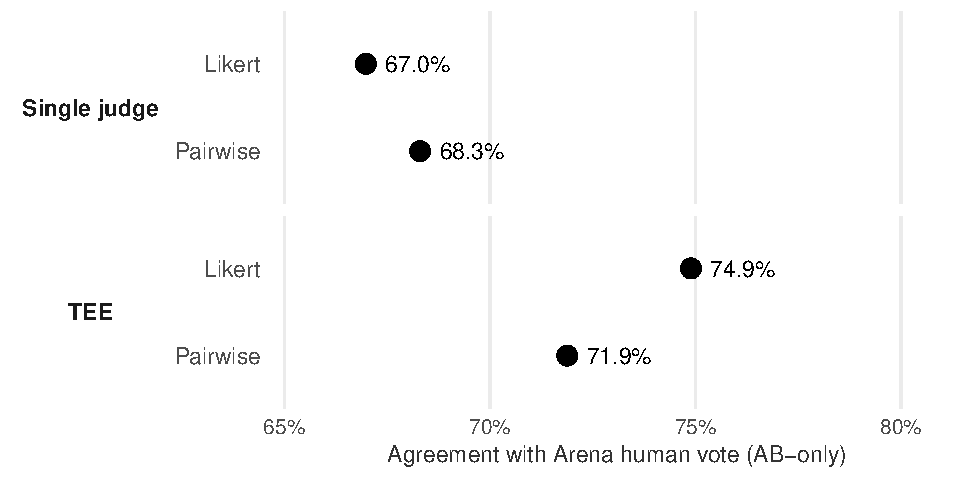
\includegraphics[width=0.9\linewidth]{fig_arena_pipeline_accuracy_dot_pooled.pdf}
\caption{TEE estimation raises agreement with Arena humans by $+7.9$ pp on Likert and $+3.6$ pp on pairwise across 4,676 matches. Each dot is one pipeline's agreement (AB-only, ties excluded).}
\label{fig:arena_accuracy}
\end{figure}

\begin{table}[ht]
\centering
\small
\caption{Agreement with Chatbot Arena human preferences by scoring pipeline and task category. \emph{Overall} counts tied predictions as correct when the human label is also a tie. \emph{AB-only} restricts to battles where both sides are decisive.}
\label{tab:arena_agreement}
\begin{tabular}{llrrrr}
\toprule
Category & Pipeline & $N$ & Overall & $N_\text{AB}$ & AB-only \\
\midrule
Creative Writing & Single-judge Likert    &    967 & 0.403 &   343 & 0.668 \\
                 & Single-judge pairwise  & 1,062 & 0.445 &   577 & 0.692 \\
                 & \textbf{TEE Likert}    & 1,064 & 0.424 &   278 & \textbf{0.763} \\
                 & TEE pairwise           & 1,064 & 0.461 &   475 & 0.743 \\
\midrule
Persuasion       & Single-judge Likert    & 1,280 & 0.362 &   327 & 0.618 \\
                 & Single-judge pairwise  & 1,426 & 0.393 &   749 & 0.621 \\
                 & \textbf{TEE Likert}    & 1,428 & 0.391 &   250 & \textbf{0.736} \\
                 & TEE pairwise           & 1,428 & 0.410 &   595 & 0.652 \\
\midrule
Coding           & Single-judge Likert    &    939 & 0.446 &   357 & 0.709 \\
                 & Single-judge pairwise  & 1,078 & 0.421 &   563 & 0.707 \\
                 & \textbf{TEE Likert}    & 1,078 & 0.449 &   351 & \textbf{0.761} \\
                 & TEE pairwise           & 1,078 & 0.441 &   482 & 0.749 \\
\midrule
Factual QA       & Single-judge Likert    & 1,006 & 0.424 &   336 & 0.682 \\
                 & Single-judge pairwise  & 1,105 & 0.474 &   597 & 0.730 \\
                 & \textbf{TEE Likert}    & 1,106 & 0.410 &   292 & \textbf{0.733} \\
                 & TEE pairwise           & 1,106 & 0.453 &   493 & 0.746 \\
\midrule
Pooled           & Single-judge Likert    & 4,192 & 0.405 & 1,363 & 0.670 \\
                 & Single-judge pairwise  & 4,671 & 0.431 & 2,486 & 0.683 \\
                 & \textbf{TEE Likert}    & 4,676 & 0.416 & 1,171 & \textbf{0.749} \\
                 & TEE pairwise           & 4,676 & 0.439 & 2,045 & 0.719 \\
\bottomrule
\end{tabular}
\end{table}

Several factors explain why TEE averaging yields a smaller accuracy gain under pairwise scoring than under Likert scoring. First, in terms of aggregation, TEE Likert averages 30 integer scores per response (one per judge$\times$variant cell) into a continuous mean, allowing two responses that a single judge tied at 4 vs.\ 4 to separate into e.g.\ 4.13 vs.\ 3.87 across the 30 cells; by contrast, TEE pairwise aggregates 30 discrete A/B/tie verdicts, which discards continuous degree-of-preference information. Second, because roughly one-third of Arena battles are human ties and our pairwise judges rarely output ties, pairwise scoring forces noisy A/B choices on tied battles that averaging cannot easily undo, whereas Likert scoring allows two responses to receive similar ratings (e.g., 3 and 3). Finally, single-judge pairwise starts from a higher baseline agreement rate than single-judge Likert because forced comparisons avoid scale quantization and anchoring effects, leaving somewhat less room for improvement from averaging.

A D-study fit on the dev split predicts the test-split lifts. For each category, we fit the lmer formula
\begin{verbatim}
score ~ (1|battle_response) + (1|variant_id) + (1|judge_model)
       + (1|battle_response:variant_id)
       + (1|battle_response:judge_model)
       + (1|variant_id:judge_model)
\end{verbatim}
on the dev split's Likert scores, then use the D-study to project per-response score SE under both a single-judge single-variant design ($V{=}1, M{=}1$) and the TEE pipeline ($V{=}5, M{=}3$). The fractional SE reductions across the four categories range 0.53 to 0.59, and the corresponding observed Likert agreement lifts on the test split range $+5.1$ to $+11.8$ pp. The two correlate at Spearman $\rho = 0.80$ (Figure~\ref{fig:arena_dstudy_vs_observed}). Persuasion has both the largest projected variance-reduction headroom and the largest observed lift.

\begin{figure}[ht]
\centering
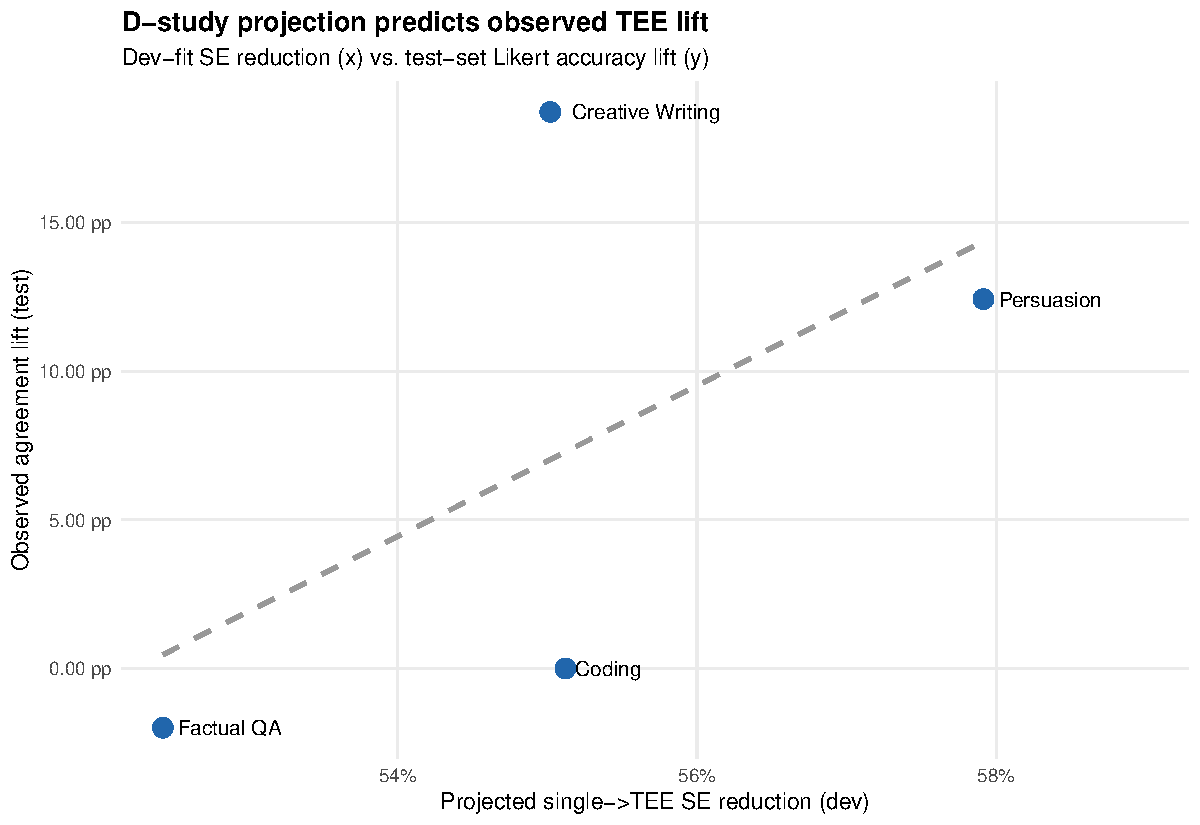
\includegraphics[width=0.85\textwidth]{fig_arena_dstudy_vs_observed.pdf}
\caption{Per-category D-study projection (dev split, x-axis) vs.\ observed Likert agreement lift (test split, y-axis). Spearman $\rho = 0.80$ across the four category points.}
\label{fig:arena_dstudy_vs_observed}
\end{figure}

At the pooled level, AB-only agreement rises from 68.3\% under single-judge pairwise to 71.9\% under TEE pairwise ($+$3.6 pp), smaller than the $+$7.9 pp Likert lift but no longer flat. The simulation in Section~\ref{si:scoring_recovery} confirms the broader pattern that Likert degrades under compression and anchoring pathologies where pairwise BT is invariant, but the present Arena dataset adds a separate calibration headwind that the simulation does not model.

Three caveats apply. First, the variance decomposition is coarser than the framework's main demonstrations because we did not vary temperature or include replications per cell, so the lmer Residual term pools the within-cell replicate noise ($\sigma^2_\rho$) with cell-level idiosyncrasy ($\sigma^2_\epsilon$). A follow-up run with three replications at temperature 1.0 on the same battles would resolve this at roughly double the API cost, and the agreement-rate headline would not change either way. Second, the LLM task categorizer has a nonzero error rate: we spot-checked 50 battles manually and found the label matched a human assessment in 44 of 50 cases (88\%). Categorical mis-tagging attenuates per-category contrasts but should not flip the subjective-vs-objective pattern. Third, roughly 20\% of Arena battles carry a tie label (including \texttt{tie (bothbad)}). The AB-only metric restricts to battles where both the human winner and the pipeline prediction are decisive. The Overall metric in Table~\ref{tab:arena_agreement} counts predicted-tie-matched-to-human-tie as correct. Both metrics support the conclusion that subjective tasks benefit most from TEE.

\subsection{Variance-coverage diagnostics}

Two further variance checks complement the per-battle agreement results. The first is a CI coverage check on the scoring-family mean at the per-battle level. The second is a bootstrap SE check on each model's BT strength at the leaderboard level. Together they probe the naive-vs-TEE gap at two levels of aggregation.

Treat the full Arena Likert factorial as a population of $4,676 \times 5 \times 3 = 70,140$ cells (battles $\times$ variants $\times$ judges). Each cell has a binary outcome $\mathtt{agree} \in \{0, 1\}$ that records whether the single-cell Likert prediction (the sign of the response-pair score difference, with a 0.5 tolerance) matches the Arena human winner. The grand mean across all cells is $p^* = 0.389$, which is the scoring-family accuracy a practitioner implicitly claims to estimate by reporting ``pipeline accuracy.''

From each of $K = 300$ Monte Carlo draws at $n_b \in \{100, 250, 500, 1,000, 2,000\}$ battles, two analysts produce a CI for $p^*$. The naive analyst picks one $(v, j)$ combo uniformly at random and reports $\hat{p} \pm 1.96 \cdot \sqrt{\hat{p}(1 - \hat{p}) / n_b}$. The TEE analyst uses all 15 cells on the same battles, fits $\mathtt{agree} \sim 1 + (1|\mathtt{battle}) + (1|\mathtt{variant}) + (1|\mathtt{judge})$, and reports the Wald CI on the intercept. Figure~\ref{si:arena_coverage} plots coverage and half-width across $n_b$.

Naive coverage falls from $0.93$ at $n_b = 100$ to $0.78$ at $n_b = 2,000$ because the binomial SE shrinks well below the variance across prompt variants and judges, causing the naive confidence interval to tighten around a single cell's mean rather than $p^*$. By contrast, TEE coverage remains at or above $0.95$ across all sample sizes (and is slightly conservative because REML estimates of $\sigma^2_V$ and $\sigma^2_J$ are noisy at $V = 5$ and $J = 3$). Practically speaking, an analyst who reports ``pipeline accuracy $= \hat{p} \pm 1$\,pp'' from $2,000$ battles using a single judge and prompt variant has roughly a 22\% chance that the full-panel accuracy lies outside their nominal $95\%$ interval—and because the omitted variance is in the standard error formula itself, adding more battles only makes the under-coverage worse.

\begin{figure}[ht]
\centering
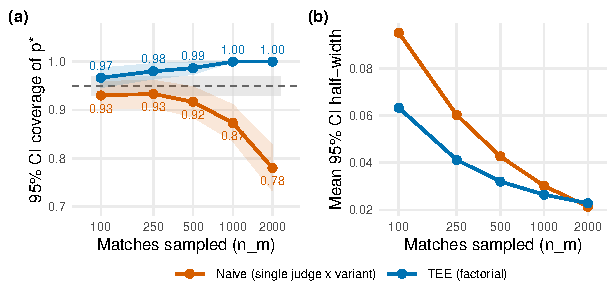
\includegraphics[width=0.78\textwidth]{fig_arena_coverage.pdf}
\caption{Naive (single judge $\times$ variant, binomial Wald) vs.\ TEE (factorial, crossed random-effects Wald) 95\% CI coverage and half-width for the scoring-family mean $p^* = 0.389$, across $K = 300$ Monte Carlo draws per $n_b$. Top: naive coverage degrades as $n_b$ grows because binomial SE shrinks past the between-cell variance floor. TEE coverage holds at or above nominal. Bottom: TEE half-width bottoms out at the $\sigma^2_V / V + \sigma^2_J / J$ floor while naive keeps shrinking. Ribbon: Monte Carlo $\pm 1.96$ SE.}
\label{si:arena_coverage}
\end{figure}

The same pattern holds at the leaderboard level. While pipeline-vs-pipeline rank correlations against the same-sample human Bradley-Terry leaderboard \citep{bradley1952rank} are not statistically distinguishable at $n = 55$ models (Spearman $\rho = 0.86$ - $0.91$ across the four pipelines, with all Williams' paired-correlation tests $p > 0.2$), the difference shows up clearly in the bootstrap standard error on each model's BT strength.

For each pipeline, we compare two bootstrap SEs for every model's BT $\log \pi_m$: a naive bootstrap that resamples the $4,676$ battles with replacement while holding each battle's pipeline prediction fixed, and a TEE-aware bootstrap that also resamples the cell design. For the single-cell pipelines, each TEE-aware replicate draws a fresh (judge, variant) cell (or (judge, variant, order) cell for pairwise) uniformly from the $15$ Likert or $30$ pairwise options and applies it to all battles in that replicate, simulating what an analyst who chose a different pipeline configuration would have reported. For the TEE pipelines, each replicate resamples the $15$ (Likert) or $30$ (pairwise) cells with replacement within each battle and re-aggregates the prediction, capturing the uncertainty from treating the observed variant and judge sets as exchangeable.

Figure~\ref{fig:arena_bt_bootstrap_se} shows the result. For the single-cell pipelines, the TEE-aware SE exceeds the naive SE by a median factor of $1.46$ (Likert) and $3.59$ (pairwise). The naive bootstrap under-reports each model's log-$\pi$ uncertainty by $32\%$ to $72\%$. For the TEE pipelines, the median ratio is $1.01$ (Likert) and $1.05$ (pairwise), confirming negligible change. Cell-level noise averages out across the 15 or 30 within-battle cells, so the BT fit is stable whether the cell set is held fixed or resampled. The per-battle coverage study (Figure~\ref{si:arena_coverage}) and this BT-level bootstrap point to the same mechanism at two levels of aggregation. Cell variance propagates directly into claims that aggregate over a single cell per battle (the naive pipelines) and averages out in proportion to the number of cells aggregated over (the TEE pipelines).

\begin{figure}[ht]
\centering
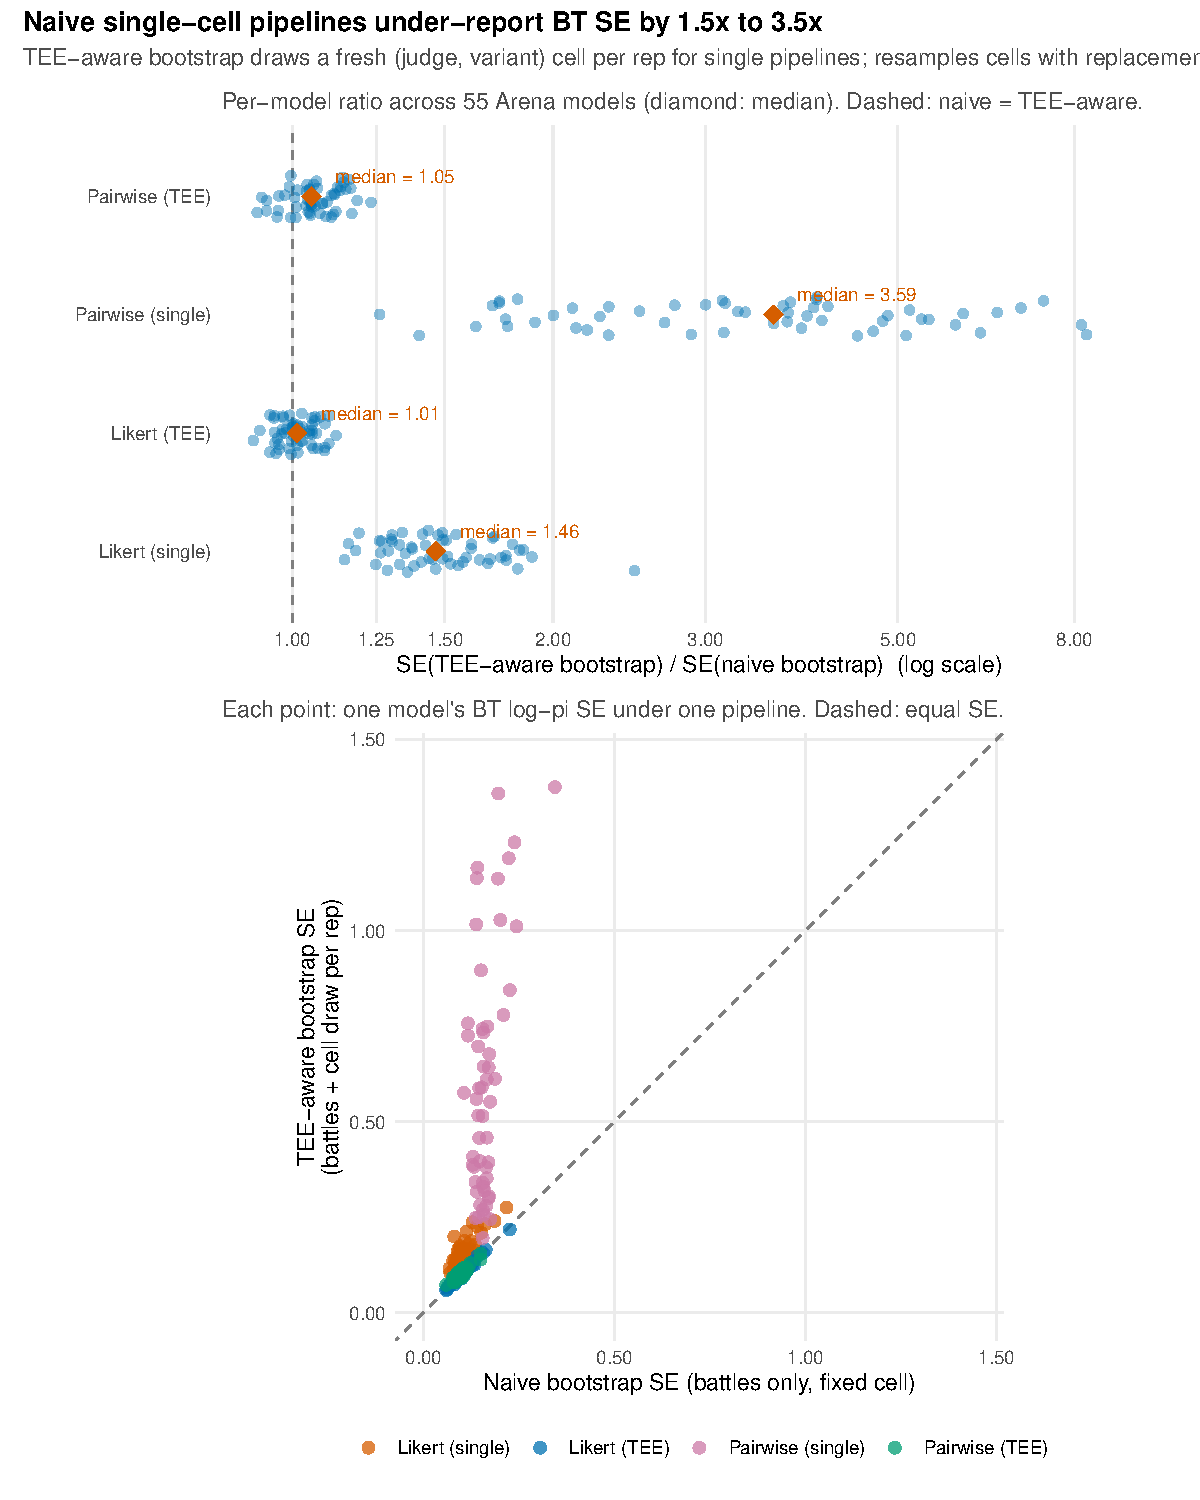
\includegraphics[width=0.85\textwidth]{fig_arena_bt_bootstrap_se.pdf}
\caption{Bootstrap SE for per-model BT $\log \pi_m$ under each of the four pipelines ($N = 300$ reps, $55$ models). Top: ratio of TEE-aware to naive bootstrap SE per model, log-scaled x-axis. Diamond is the per-pipeline median. Bottom: scatter of naive vs.\ TEE-aware SE. Dashed line is equality. Single-cell pipelines cluster above the diagonal (naive under-estimates). TEE pipelines cluster on the diagonal (cell variance is absorbed by aggregation).}
\label{fig:arena_bt_bootstrap_se}
\end{figure}


\newpage
% NeurIPS 2026 Paper Checklist. Questions and guidelines are verbatim from the official
% template (Formatting_Instructions_For_NeurIPS_2026.zip, checklist.tex); answers are ours.
% Included by neurips_main.tex after the appendix, as in the template.
\section*{NeurIPS Paper Checklist}



\begin{enumerate}

\item {\bf Claims}
    \item[] Question: Do the main claims made in the abstract and introduction accurately reflect the paper's contributions and scope?
    \item[] Answer: \answerYes{}
    \item[] Justification: The abstract and introduction state three contributions (variance decomposition, fixed-random effect separation, D-study projections) and the headline empirical findings (53 - 70\% naive SE underestimate in the judge-scored safety and ideology demonstrations; roughly halving MMLU error at equal cost; cutting the Arena best-of-27 gaming surface from 56 to 32 Elo; 7.9-point Arena human-vote agreement lift). Each is supported by a corresponding section: \S\ref{sec:framework} for the decomposition and D-study, \S\ref{sec:safety} - \S\ref{sec:gaming} for the empirical claims, and SI Section~\ref{si:naive_vs_tee} for the SE comparison.
    \item[] Guidelines:
    \begin{itemize}
        \item The answer \answerNA{} means that the abstract and introduction do not include the claims made in the paper.
        \item The abstract and/or introduction should clearly state the claims made, including the contributions made in the paper and important assumptions and limitations. A \answerNo{} or \answerNA{} answer to this question will not be perceived well by the reviewers. 
        \item The claims made should match theoretical and experimental results, and reflect how much the results can be expected to generalize to other settings. 
        \item It is fine to include aspirational goals as motivation as long as it is clear that these goals are not attained by the paper. 
    \end{itemize}

\item {\bf Limitations}
    \item[] Question: Does the paper discuss the limitations of the work performed by the authors?
    \item[] Answer: \answerYes{}
    \item[] Justification: \S\ref{sec:limitations} discusses cost, English-only and frontier scope, coverage error vs.\ TEE, reasoning-trace variance, recursive judge measurement error, tier-matched judge sensitivity, cross-layer interactions, and LPM vs.\ GLMM scaling.
    \item[] Guidelines:
    \begin{itemize}
        \item The answer \answerNA{} means that the paper has no limitation while the answer \answerNo{} means that the paper has limitations, but those are not discussed in the paper. 
        \item The authors are encouraged to create a separate ``Limitations'' section in their paper.
        \item The paper should point out any strong assumptions and how robust the results are to violations of these assumptions (e.g., independence assumptions, noiseless settings, model well-specification, asymptotic approximations only holding locally). The authors should reflect on how these assumptions might be violated in practice and what the implications would be.
        \item The authors should reflect on the scope of the claims made, e.g., if the approach was only tested on a few datasets or with a few runs. In general, empirical results often depend on implicit assumptions, which should be articulated.
        \item The authors should reflect on the factors that influence the performance of the approach. For example, a facial recognition algorithm may perform poorly when image resolution is low or images are taken in low lighting. Or a speech-to-text system might not be used reliably to provide closed captions for online lectures because it fails to handle technical jargon.
        \item The authors should discuss the computational efficiency of the proposed algorithms and how they scale with dataset size.
        \item If applicable, the authors should discuss possible limitations of their approach to address problems of privacy and fairness.
        \item While the authors might fear that complete honesty about limitations might be used by reviewers as grounds for rejection, a worse outcome might be that reviewers discover limitations that aren't acknowledged in the paper. The authors should use their best judgment and recognize that individual actions in favor of transparency play an important role in developing norms that preserve the integrity of the community. Reviewers will be specifically instructed to not penalize honesty concerning limitations.
    \end{itemize}

\item {\bf Theory assumptions and proofs}
    \item[] Question: For each theoretical result, does the paper provide the full set of assumptions and a complete (and correct) proof?
    \item[] Answer: \answerYes{}
    \item[] Justification: The DGP and decomposition rest on three named assumptions (conditional exchangeability, additivity with two-way interactions, normally distributed independent random effects), stated in \S\ref{sec:framework} and elaborated in SI Appendix \S\ref{si:framework}. Monte Carlo robustness checks against violations of each assumption are reported in SI Appendix \S\ref{si:dstudy_validation} and \S\ref{si:latent_ambiguity}.
    \item[] Guidelines:
    \begin{itemize}
        \item The answer \answerNA{} means that the paper does not include theoretical results. 
        \item All the theorems, formulas, and proofs in the paper should be numbered and cross-referenced.
        \item All assumptions should be clearly stated or referenced in the statement of any theorems.
        \item The proofs can either appear in the main paper or the supplemental material, but if they appear in the supplemental material, the authors are encouraged to provide a short proof sketch to provide intuition. 
        \item Inversely, any informal proof provided in the core of the paper should be complemented by formal proofs provided in appendix or supplemental material.
        \item Theorems and Lemmas that the proof relies upon should be properly referenced. 
    \end{itemize}

    \item {\bf Experimental result reproducibility}
    \item[] Question: Does the paper fully disclose all the information needed to reproduce the main experimental results of the paper to the extent that it affects the main claims and/or conclusions of the paper (regardless of whether the code and data are provided or not)?
    \item[] Answer: \answerYes{}
    \item[] Justification: Each demonstration specifies the full factorial design (item counts, prompt variants, judges, temperatures, replications, models), the REML estimator and \texttt{lmer} formula (\S\ref{sec:framework}), and the GUIDE-LLM disclosure (SI Appendix \S\ref{si:llm_disclosure}). Simulation parameters and code paths are listed in SI Appendix \S\ref{si:simulations}.
    \item[] Guidelines:
    \begin{itemize}
        \item The answer \answerNA{} means that the paper does not include experiments.
        \item If the paper includes experiments, a \answerNo{} answer to this question will not be perceived well by the reviewers: Making the paper reproducible is important, regardless of whether the code and data are provided or not.
        \item If the contribution is a dataset and\slash or model, the authors should describe the steps taken to make their results reproducible or verifiable. 
        \item Depending on the contribution, reproducibility can be accomplished in various ways. For example, if the contribution is a novel architecture, describing the architecture fully might suffice, or if the contribution is a specific model and empirical evaluation, it may be necessary to either make it possible for others to replicate the model with the same dataset, or provide access to the model. In general. releasing code and data is often one good way to accomplish this, but reproducibility can also be provided via detailed instructions for how to replicate the results, access to a hosted model (e.g., in the case of a large language model), releasing of a model checkpoint, or other means that are appropriate to the research performed.
        \item While NeurIPS does not require releasing code, the conference does require all submissions to provide some reasonable avenue for reproducibility, which may depend on the nature of the contribution. For example
        \begin{enumerate}
            \item If the contribution is primarily a new algorithm, the paper should make it clear how to reproduce that algorithm.
            \item If the contribution is primarily a new model architecture, the paper should describe the architecture clearly and fully.
            \item If the contribution is a new model (e.g., a large language model), then there should either be a way to access this model for reproducing the results or a way to reproduce the model (e.g., with an open-source dataset or instructions for how to construct the dataset).
            \item We recognize that reproducibility may be tricky in some cases, in which case authors are welcome to describe the particular way they provide for reproducibility. In the case of closed-source models, it may be that access to the model is limited in some way (e.g., to registered users), but it should be possible for other researchers to have some path to reproducing or verifying the results.
        \end{enumerate}
    \end{itemize}


\item {\bf Open access to data and code}
    \item[] Question: Does the paper provide open access to the data and code, with sufficient instructions to faithfully reproduce the main experimental results, as described in supplemental material?
    \item[] Answer: \answerYes{}
    \item[] Justification: Replication code, processed data, and a reproduction README are at \url{https://github.com/SolomonMg/totalevalerror-replication}, and the R package implementing the method is at \url{https://github.com/SolomonMg/totalevalerror}. Raw API responses (JSONL) are archived on Harvard Dataverse, linked from the repository README.
    \item[] Guidelines:
    \begin{itemize}
        \item The answer \answerNA{} means that paper does not include experiments requiring code.
        \item Please see the NeurIPS code and data submission guidelines (\url{https://neurips.cc/public/guides/CodeSubmissionPolicy}) for more details.
        \item While we encourage the release of code and data, we understand that this might not be possible, so \answerNo{} is an acceptable answer. Papers cannot be rejected simply for not including code, unless this is central to the contribution (e.g., for a new open-source benchmark).
        \item The instructions should contain the exact command and environment needed to run to reproduce the results. See the NeurIPS code and data submission guidelines (\url{https://neurips.cc/public/guides/CodeSubmissionPolicy}) for more details.
        \item The authors should provide instructions on data access and preparation, including how to access the raw data, preprocessed data, intermediate data, and generated data, etc.
        \item The authors should provide scripts to reproduce all experimental results for the new proposed method and baselines. If only a subset of experiments are reproducible, they should state which ones are omitted from the script and why.
        \item At submission time, to preserve anonymity, the authors should release anonymized versions (if applicable).
        \item Providing as much information as possible in supplemental material (appended to the paper) is recommended, but including URLs to data and code is permitted.
    \end{itemize}


\item {\bf Experimental setting/details}
    \item[] Question: Does the paper specify all the training and test details (e.g., data splits, hyperparameters, how they were chosen, type of optimizer) necessary to understand the results?
    \item[] Answer: \answerYes{}
    \item[] Justification: \S\ref{sec:framework} specifies the lmer formula, REML estimation, fixed vs.\ random effects, and prompt-variant generation procedure. SI Appendix \S\ref{si:framework} gives the full \texttt{lmer} call. Each empirical section names the specific models, prompts, temperature settings, and replication counts.
    \item[] Guidelines:
    \begin{itemize}
        \item The answer \answerNA{} means that the paper does not include experiments.
        \item The experimental setting should be presented in the core of the paper to a level of detail that is necessary to appreciate the results and make sense of them.
        \item The full details can be provided either with the code, in appendix, or as supplemental material.
    \end{itemize}

\item {\bf Experiment statistical significance}
    \item[] Question: Does the paper report error bars suitably and correctly defined or other appropriate information about the statistical significance of the experiments?
    \item[] Answer: \answerYes{}
    \item[] Justification: All empirical confidence intervals are 95\% Wald intervals based on REML variance components (\S\ref{sec:framework}, equation \ref{eq:dstudy_multi}). Parametric bootstrap CIs are used when facet counts are small (SI Appendix \S\ref{si:checklist}). Monte Carlo studies use 1{,}000 simulation replicates (SI Appendix \S\ref{si:simulations}).
    \item[] Guidelines:
    \begin{itemize}
        \item The answer \answerNA{} means that the paper does not include experiments.
        \item The authors should answer \answerYes{} if the results are accompanied by error bars, confidence intervals, or statistical significance tests, at least for the experiments that support the main claims of the paper.
        \item The factors of variability that the error bars are capturing should be clearly stated (for example, train/test split, initialization, random drawing of some parameter, or overall run with given experimental conditions).
        \item The method for calculating the error bars should be explained (closed form formula, call to a library function, bootstrap, etc.)
        \item The assumptions made should be given (e.g., Normally distributed errors).
        \item It should be clear whether the error bar is the standard deviation or the standard error of the mean.
        \item It is OK to report 1-sigma error bars, but one should state it. The authors should preferably report a 2-sigma error bar than state that they have a 96\% CI, if the hypothesis of Normality of errors is not verified.
        \item For asymmetric distributions, the authors should be careful not to show in tables or figures symmetric error bars that would yield results that are out of range (e.g., negative error rates).
        \item If error bars are reported in tables or plots, the authors should explain in the text how they were calculated and reference the corresponding figures or tables in the text.
    \end{itemize}

\item {\bf Experiments compute resources}
    \item[] Question: For each experiment, does the paper provide sufficient information on the computer resources (type of compute workers, memory, time of execution) needed to reproduce the experiments?
    \item[] Answer: \answerYes{}
    \item[] Justification: API-based experiments cost approximately \$92 in OpenRouter spend across the safety, MMLU, and ideology demonstrations. Monte Carlo simulations were run on a single HPC node for the variance-underestimation simulation (\S\ref{si:underestimation_sim}) and on a workstation (Apple Silicon) for the remaining studies; per-script wall-clock estimates are reported in the reproduction README.
    \item[] Guidelines:
    \begin{itemize}
        \item The answer \answerNA{} means that the paper does not include experiments.
        \item The paper should indicate the type of compute workers CPU or GPU, internal cluster, or cloud provider, including relevant memory and storage.
        \item The paper should provide the amount of compute required for each of the individual experimental runs as well as estimate the total compute. 
        \item The paper should disclose whether the full research project required more compute than the experiments reported in the paper (e.g., preliminary or failed experiments that didn't make it into the paper). 
    \end{itemize}
    
\item {\bf Code of ethics}
    \item[] Question: Does the research conducted in the paper conform, in every respect, with the NeurIPS Code of Ethics \url{https://neurips.cc/public/EthicsGuidelines}?
    \item[] Answer: \answerYes{}
    \item[] Justification: All benchmark items come from public datasets (AILuminate v1.0, MMLU, Chatbot Arena, propaganda audit). No new human subjects were recruited; the propaganda human ratings come from prior published research with original IRB approval. No personally identifiable information was collected or processed.
    \item[] Guidelines:
    \begin{itemize}
        \item The answer \answerNA{} means that the authors have not reviewed the NeurIPS Code of Ethics.
        \item If the authors answer \answerNo, they should explain the special circumstances that require a deviation from the Code of Ethics.
        \item The authors should make sure to preserve anonymity (e.g., if there is a special consideration due to laws or regulations in their jurisdiction).
    \end{itemize}


\item {\bf Broader impacts}
    \item[] Question: Does the paper discuss both potential positive societal impacts and negative societal impacts of the work performed?
    \item[] Answer: \answerYes{}
    \item[] Justification: \S\ref{sec:discussion} discusses the deployment, safety-certification, and regulatory consequences of underestimating evaluation uncertainty. The gaming analysis (\S\ref{sec:gaming}) identifies how unmeasured pipeline variance lets developers inflate benchmark scores; tightening the variance accounting reduces both the false-precision risk and the gaming surface.
    \item[] Guidelines:
    \begin{itemize}
        \item The answer \answerNA{} means that there is no societal impact of the work performed.
        \item If the authors answer \answerNA{} or \answerNo, they should explain why their work has no societal impact or why the paper does not address societal impact.
        \item Examples of negative societal impacts include potential malicious or unintended uses (e.g., disinformation, generating fake profiles, surveillance), fairness considerations (e.g., deployment of technologies that could make decisions that unfairly impact specific groups), privacy considerations, and security considerations.
        \item The conference expects that many papers will be foundational research and not tied to particular applications, let alone deployments. However, if there is a direct path to any negative applications, the authors should point it out. For example, it is legitimate to point out that an improvement in the quality of generative models could be used to generate Deepfakes for disinformation. On the other hand, it is not needed to point out that a generic algorithm for optimizing neural networks could enable people to train models that generate Deepfakes faster.
        \item The authors should consider possible harms that could arise when the technology is being used as intended and functioning correctly, harms that could arise when the technology is being used as intended but gives incorrect results, and harms following from (intentional or unintentional) misuse of the technology.
        \item If there are negative societal impacts, the authors could also discuss possible mitigation strategies (e.g., gated release of models, providing defenses in addition to attacks, mechanisms for monitoring misuse, mechanisms to monitor how a system learns from feedback over time, improving the efficiency and accessibility of ML).
    \end{itemize}
    
\item {\bf Safeguards}
    \item[] Question: Does the paper describe safeguards that have been put in place for responsible release of data or models that have a high risk for misuse (e.g., pre-trained language models, image generators, or scraped datasets)?
    \item[] Answer: \answerNA{}
    \item[] Justification: The paper releases no model weights, no harmful training data, and no exploitation tools. It releases evaluation methodology and code for variance estimation.
    \item[] Guidelines:
    \begin{itemize}
        \item The answer \answerNA{} means that the paper poses no such risks.
        \item Released models that have a high risk for misuse or dual-use should be released with necessary safeguards to allow for controlled use of the model, for example by requiring that users adhere to usage guidelines or restrictions to access the model or implementing safety filters. 
        \item Datasets that have been scraped from the Internet could pose safety risks. The authors should describe how they avoided releasing unsafe images.
        \item We recognize that providing effective safeguards is challenging, and many papers do not require this, but we encourage authors to take this into account and make a best faith effort.
    \end{itemize}

\item {\bf Licenses for existing assets}
    \item[] Question: Are the creators or original owners of assets (e.g., code, data, models), used in the paper, properly credited and are the license and terms of use explicitly mentioned and properly respected?
    \item[] Answer: \answerYes{}
    \item[] Justification: AILuminate v1.0 (MLCommons), MMLU, Chatbot Arena Conversations, and the propaganda dataset are cited at first use; their respective licenses are observed. The R package \texttt{lme4} \citep{bates2015lme4} is cited.
    \item[] Guidelines:
    \begin{itemize}
        \item The answer \answerNA{} means that the paper does not use existing assets.
        \item The authors should cite the original paper that produced the code package or dataset.
        \item The authors should state which version of the asset is used and, if possible, include a URL.
        \item The name of the license (e.g., CC-BY 4.0) should be included for each asset.
        \item For scraped data from a particular source (e.g., website), the copyright and terms of service of that source should be provided.
        \item If assets are released, the license, copyright information, and terms of use in the package should be provided. For popular datasets, \url{paperswithcode.com/datasets} has curated licenses for some datasets. Their licensing guide can help determine the license of a dataset.
        \item For existing datasets that are re-packaged, both the original license and the license of the derived asset (if it has changed) should be provided.
        \item If this information is not available online, the authors are encouraged to reach out to the asset's creators.
    \end{itemize}

\item {\bf New assets}
    \item[] Question: Are new assets introduced in the paper well documented and is the documentation provided alongside the assets?
    \item[] Answer: \answerYes{}
    \item[] Justification: The released code includes a reproduction README, a \texttt{requirements.txt}, the \texttt{config.py} that controls the staged design (smoke / pilot / full), and inline documentation in each analysis script. Processed CSVs include column descriptions.
    \item[] Guidelines:
    \begin{itemize}
        \item The answer \answerNA{} means that the paper does not release new assets.
        \item Researchers should communicate the details of the dataset\slash code\slash model as part of their submissions via structured templates. This includes details about training, license, limitations, etc. 
        \item The paper should discuss whether and how consent was obtained from people whose asset is used.
        \item At submission time, remember to anonymize your assets (if applicable). You can either create an anonymized URL or include an anonymized zip file.
    \end{itemize}

\item {\bf Crowdsourcing and research with human subjects}
    \item[] Question: For crowdsourcing experiments and research with human subjects, does the paper include the full text of instructions given to participants and screenshots, if applicable, as well as details about compensation (if any)? 
    \item[] Answer: \answerNA{}
    \item[] Justification: No new human-subjects data collection was conducted. The propaganda demonstration uses ratings from a prior published study; that study's instructions and compensation are documented in its original publication.
    \item[] Guidelines:
    \begin{itemize}
        \item The answer \answerNA{} means that the paper does not involve crowdsourcing nor research with human subjects.
        \item Including this information in the supplemental material is fine, but if the main contribution of the paper involves human subjects, then as much detail as possible should be included in the main paper. 
        \item According to the NeurIPS Code of Ethics, workers involved in data collection, curation, or other labor should be paid at least the minimum wage in the country of the data collector. 
    \end{itemize}

\item {\bf Institutional review board (IRB) approvals or equivalent for research with human subjects}
    \item[] Question: Does the paper describe potential risks incurred by study participants, whether such risks were disclosed to the subjects, and whether Institutional Review Board (IRB) approvals (or an equivalent approval/review based on the requirements of your country or institution) were obtained?
    \item[] Answer: \answerNA{}
    \item[] Justification: No new human-subjects data collection. Pre-existing human ratings used for validation come from research with original IRB approval, cited in the corresponding source publication.
    \item[] Guidelines:
    \begin{itemize}
        \item The answer \answerNA{} means that the paper does not involve crowdsourcing nor research with human subjects.
        \item Depending on the country in which research is conducted, IRB approval (or equivalent) may be required for any human subjects research. If you obtained IRB approval, you should clearly state this in the paper. 
        \item We recognize that the procedures for this may vary significantly between institutions and locations, and we expect authors to adhere to the NeurIPS Code of Ethics and the guidelines for their institution. 
        \item For initial submissions, do not include any information that would break anonymity (if applicable), such as the institution conducting the review.
    \end{itemize}

\item {\bf Declaration of LLM usage}
    \item[] Question: Does the paper describe the usage of LLMs if it is an important, original, or non-standard component of the core methods in this research? Note that if the LLM is used only for writing, editing, or formatting purposes and does \emph{not} impact the core methodology, scientific rigor, or originality of the research, declaration is not required.
    %this research? 
    \item[] Answer: \answerYes{}
    \item[] Justification: LLMs are the object of study, not just a writing aid. Multiple LLM judge models and SUTs were accessed via the OpenRouter API across the four demonstrations, with per-demonstration model identifiers, parameters, and prompt texts reported in SI Appendix \S\ref{si:llm_disclosure} following the GUIDE-LLM checklist \citep{feuerriegel2026guidellm}. Prompt variants were also generated by an LLM (SI Appendix \S\ref{si:framework}). An LLM coding assistant supported data collection scripts, analysis pipeline development, simulation implementation, and manuscript preparation. The author is solely responsible for the accuracy of all content.
    \item[] Guidelines:
    \begin{itemize}
        \item The answer \answerNA{} means that the core method development in this research does not involve LLMs as any important, original, or non-standard components.
        \item Please refer to our LLM policy in the NeurIPS handbook for what should or should not be described.
    \end{itemize}

\end{enumerate}


\end{document}
